\documentclass{beamer}
\usepackage{alltt}
\usepackage{tikz}
\usetikzlibrary{matrix}
\usetikzlibrary{trees}
\usepackage{cancel}
\usepackage{subcaption}
\PassOptionsToPackage{obeyspaces}{url}
\usepackage{hyperref}
\usepackage{adjustbox}

\usetheme{Hannover}

\newcommand{\racket}{\texttt{Racket}}
\newcommand{\drr}{\texttt{DrRacket}}
\newcommand{\fsm}{\texttt{FSM}}
\newcommand{\ide}{\texttt{IDE}}
\newcommand{\api}{\texttt{API}}
\newcommand{\arrow}{\(\rightarrow\)}
\newcommand{\dotss}{\(\ldots\)}
\newcommand{\vdotss}{\(\vdots\)}
\newcommand{\elist}{\texttt{\textquotesingle{()}}}
\newcommand{\logand}{\texttt{\(\wedge\)}}
\newcommand{\logor}{\texttt{\(\vee\)}}
%\newcommand{\emptyset}{\texttt{\(\varnothing\)}}
\newcommand{\sig}{\texttt{\(\Sigma\)}}
\newcommand{\delt}{\texttt{\(\delta\)}}
\newcommand{\sigsig}{\texttt{\(\Sigma\) = \{a b\}}}
\newcommand{\gam}{\texttt{\(\Gamma\)}}
\newcommand{\ep}{\texttt{\(\epsilon\)}}
\newcommand{\quot}{\texttt{\textquotesingle{}}}
\newcommand{\dquot}{\texttt{"}}
\newcommand{\qquot}{\texttt{\textasciigrave{}}}
\newcommand{\lambexpr}{\texttt{$\lambda$}-expression}
\newcommand{\lamb}{\texttt{$\lambda$}}
\newcommand{\accept}{\texttt{\textquotesingle{}accept}}
\newcommand{\reject}{\texttt{\textquotesingle{}reject}}
\newcommand{\dfa}{\texttt{dfa}}
\newcommand{\ndfa}{\texttt{ndfa}}
\newcommand{\pda}{\texttt{pda}}
\newcommand{\tm}{\texttt{tm}}
\newcommand{\mttm}{\texttt{mttm}}
\newcommand{\step}{\texttt{$\vdash$}}
\newcommand{\steps}{\texttt{$\vdash^*$}}
\newcommand{\gstep}{\texttt{$\rightarrow$}}
\newcommand{\gsteps}{\texttt{$\rightarrow^+$}}
\newcommand{\utm}{\texttt{UTM}}
\newcommand{\ctm}{\texttt{ctm}}
\newcommand{\ci}{\texttt{ci}}
\newcommand{\ffbox}[1]{%
  {% open a group for a local setting
   \setlength{\fboxsep}{-2\fboxrule}% the rule will be inside the box boundary
   \fbox{\hspace{1.2pt}\strut#1\hspace{1.2pt}}% print the box, with some padding at the left and right
  }% close the group
}
\newcommand{\ets}{\texttt{$\epsilon$}-transitions}
\newcommand{\et}{\texttt{$\epsilon$}-transition}
\newcommand{\rg}{\texttt{rg}}
\newcommand{\cfg}{\texttt{cfg}}
\newcommand{\csg}{\texttt{csg}}

\definecolor{darkgreen}{RGB}{102,170,102}

\begin{document}

\title{Part II: Regular Languages}
%\subtitle{Using Beamer}
\author{Marco T. Moraz\'{a}n}
\institute{Seton Hall University}
\date{}

\begin{frame}
\titlepage
\end{frame}

\begin{frame}
\frametitle{Outline}
\tableofcontents
\end{frame}

\section{Regular Expressions}

\begin{frame}[fragile]
\frametitle{Regular Expressions}
%\framesubtitle{HOMEWORK}
\begin{scriptsize}
\begin{itemize}
\item<1-> An English word is a string of juxtaposed letters found in the Roman alphabet: \texttt{[a..z]}

\item<1-> As a Computer Science student and reader of this textbook, you are familiar with other languages

\item<2-> Defining English words as strings is a representation choice

\item<2-> Consider three different representations of the word \textsl{cat}:
\begin{alltt}
     English: "cat"
         FSM: \quot(c a t)
      Binary: 011000110110000101110100
\end{alltt}

\item<2-> The representations of \textsl{cat} are different, but the same concept is being represented.

\item<3-> A language may, for example, be represented as a set of strings, a set of lists, or a set of binary numbers

\item<3-> Regardless of the representation, the same words in the English language are represented.

\end{itemize}
\end{scriptsize}
\end{frame}

\begin{frame}[fragile]
\frametitle{Regular Expressions}
%\framesubtitle{HOMEWORK}
\begin{scriptsize}
\begin{itemize}
\item<1-> Languages are represented using a finite representation

\item<1-> If a language is finite listing all the words in the language is a finite representation

\item<1-> A finite representation for infinite languages is needed because all the words in an infinite language cannot be listed

\item<2-> A finite representation for a language must be written using a finite number of symbols

\item<2-> If \texttt{$\Sigma$} is an alphabet used to write the finite representations of languages then all possible finite language representations are defined as \texttt{$\Sigma^{\texttt{*}}$}

\item<2-> This means that the language of finite language representations is countably infinite

\item<3-> \texttt{2$^{\texttt{$\Sigma^{\texttt{*}}$}}$}, however, is uncountable

\item<3-> There is a countable number of finite language representations and an uncountable number of languages to represent

\item<4-> Therefore, a finite representation for each language does not exist

\item<4-> The best that we can achieve is to develop a finite representation of some interesting languages

\item<4-> As long as a representation is finite the majority of languages cannot be represented.

\end{itemize}
\end{scriptsize}
\end{frame}

\begin{frame}[fragile]
\frametitle{Regular Expressions}
%\framesubtitle{HOMEWORK}
\begin{scriptsize}
\begin{itemize}
\item<1-> We start by considering languages formed by the union or the concatenation of words in two (not necessarily distinct) languages

\item<1-> Such languages may be finitely represented using regular expressions

\item<2-> A regular expression, over an alphabet \sig, is an \fsm{} type instance:
\begin{alltt}
    1. (empty-regexp)
    2. (singleton-regexp "a"), where a\(\in\)\(\Sigma\)
    3. (union-regexp r1 r2),  where r1 and r2 are regular
                              expressions
    4. (concat-regexp r1 r2), where r1 and r2 are regular
                              expressions
    5. (kleenestar-regexp r), where r is a regular expression
\end{alltt}

\item<2-> The language of a regular expression, \texttt{r}, is denoted by \texttt{L(r)}

\item<2-> It contains all the words that can be generated with \texttt{r}

\item<2-> A language that is described by a regular expression is called a \emph{regular language}.

\end{itemize}
\end{scriptsize}
\end{frame}

\begin{frame}[fragile]
\frametitle{Regular Expressions}
%\framesubtitle{HOMEWORK}
\begin{scriptsize}
The Design Recipe for Regular Expressions
\begin{enumerate}
     \item Identify the input alphabet, pick a name for the regular expression, and describe the language
     
     \item Identify the sublanguages and outline how to compose them
     
     \item Define a predicate to determine if a word is in the target language
     
     \item Write unit tests
     
     \item Define the regular expression
     
     \item Run the tests and, if necessary, debug by revisiting the previous steps
     \item Prove that the regular expression is correct
\end{enumerate}
\end{scriptsize}
\end{frame}

\begin{frame}[fragile]
\frametitle{Regular Expressions}
%\framesubtitle{HOMEWORK}
\begin{scriptsize}
\begin{itemize}
\item<1-> \fsm{} provides \emph{recipe-based error messages}\footnote{This term was coined by Prof. Rose Bohrer from WPI.} for constructor misuse

\item<2->
\begin{alltt}
> (union-regexp 2 (singleton-regexp \textquotesingle{}w))
\textcolor{red}{Step five of the design recipe for regular expressions 
has not been successfully completed. The argument to 
singleton-regexp must be a single lowercase Roman alphabet
string, but found: w}
\end{alltt}

\item<3->
\begin{alltt}
> (union-regexp 2 (singleton-regexp "w"))
\textcolor{red}{Step five of the design recipe for regular expressions 
has not been successfully completed. The first argument 
to union-regexpmust be a regular expression, but found: 2}
\end{alltt}

\item<4->
\begin{alltt}
> (concat-regexp 3 (empty-regexp))
\textcolor{red}{Step five of the design recipe for regular expressions 
has not been successfully completed. The first argument 
to concat-regexp must be a regular expression, but found: 3}
\end{alltt}

\item<5->
\begin{alltt}
> (kleenestar-regexp "A U B")
\textcolor{red}{Step five of the design recipe for regular expressions 
has not been successfully completed. The argument to 
kleenestar-regexp must be a regular expression, but found: "A U B"}
\end{alltt}

\item<6->
\begin{alltt}
> (singleton-regexp 1)
\textcolor{red}{Step five of the design recipe for regular 
expressions has not been successfully completed. The argument 
to singleton-regexp must be a single lowercase Roman alphabet 
string, but found: 1}
\end{alltt}

\end{itemize}
\end{scriptsize}
\end{frame}

\begin{frame}[fragile]
\frametitle{Regular Expressions}
%\framesubtitle{HOMEWORK}
\begin{scriptsize}
\begin{itemize}
\item<1-> Selectors and Predicates

\item<2->
\begin{description}
  \item[\underline{singleton-regexp-a}:] Extracts the embedded string
  \item[\underline{kleenestar-regexp-r1}:] Extracts the embedded regular expression
  \item[\underline{union-regexp-r1}:] Extracts the first embedded regular expression
  \item[\underline{union-regexp-r2}:] Extracts the second embedded regular expression
  \item[\underline{concat-regexp-r1}:] Extracts the first embedded regular expression
  \item[\underline{concat-regexp-r2}:] Extracts the second embedded regular expression
\end{description}

\item<3->
\begin{alltt}
     empty-regexp?     singleton-regexp     kleenestar-regexp?
     union-regexp?     concat-regexp?
\end{alltt}

\item<4-> Function Template
\begin{alltt}
   ;; regexp \dotss \arrow \dotss
   ;; Purpose: \dotss
   (define (f-on-regexp rexp \dotss)
     (cond [(empty-regexp? rexp) \dotss]
           [(singleton-regexp? rexp)
            \dotss(f-on-string (singleton-regexp-a rexp))\dotss]
           [(kleenestar-regexp? rexp)
            \dotss(f-on-regexp (kleenestar-regexp-r1 rexp))\dotss]
           [(union-regexp? rexp)
            \dotss(f-on-regexp (union-regexp-r1 rexp))\dotss
            \dotss(f-on-regexp (union-regexp-r2 rexp))\dotss]
           [else \dotss(f-on-regexp (concat-regexp-r1 rexp))\dotss
                 \dotss(f-on-regexp (concat-regexp-r2 rexp))\dotss]))
\end{alltt}

\end{itemize}
\end{scriptsize}
\end{frame}

\begin{frame}[fragile]
\frametitle{Regular Expressions}
%\framesubtitle{HOMEWORK}
\begin{scriptsize}
\begin{itemize}
\item<1-> Observers for regular expressions
\begin{description}
  \item[\underline{(gen-regexp-word r)}:] Nondeterministically generates a word in the language of the given \texttt{regexp}.
\end{description}

\item<1-> Many more available for you to write your own \texttt{gen-word-regexp} (see documentation)

\end{itemize}
\end{scriptsize}
\end{frame}

\begin{frame}[fragile]
\frametitle{Regular Expressions}
%\framesubtitle{HOMEWORK}
\begin{scriptsize}
\begin{itemize}
\item<1-> \fsm{} provides \texttt{printable-regexp}:

\item<1->
\begin{alltt}
> (printable-regexp (empty-regexp))
"\(\epsilon\)"
> (printable-regexp (singleton-regexp "z"))
"z"
> (printable-regexp
   (union-regexp (singleton-regexp "z") (union-regexp
                                         (singleton-regexp "1")
                                         (singleton-regexp "q"))))
"(z U (1 U q))"
> (printable-regexp
   (concat-regexp (singleton-regexp "i") (singleton-regexp "i")))
"ii"
> (printable-regexp
   (kleenestar-regexp (concat-regexp (singleton-regexp "a")
                                     (singleton-regexp "b"))))
"(ab)\(\sp{*}\)"
\end{alltt}

\end{itemize}
\end{scriptsize}
\end{frame}

\begin{frame}[fragile]
\frametitle{Regular Expressions}
%\framesubtitle{HOMEWORK}
\begin{tiny}
\begin{itemize}
\item<1-> Consider the following language over \sigsig: \texttt{L = \{w $|$ w ends with an a\}}
    
\item<1-> Design idea: Concatenate any word with a

\item<4->
\begin{alltt}
;; word --> Boolean
;; Purpose: Determine if given word is in L(ENDS-WITH-A)
(define (valid-ends-with-a? w)
  (and (eq? (last w) \quot{}a)
       (andmap (\lamb{} (l) (or (eq? l \quot{}a) (eq? l \quot{}b))) w)))
\end{alltt}

\item<2->
\begin{alltt}
 #lang fsm

;; L(ENDS-WITH-A) = All words that end with an a   Alphabet = {a b}
(define ENDS-WITH-A
\end{alltt}

\item<6->
\begin{alltt}
  (local [;; L(A) = {(a)}   Alphabet = {a}
          (define A (singleton-regexp "a"))

          ;; L(B) = {b}   Alphabet = {(b)}
          (define B (singleton-regexp "b"))
          
\end{alltt}

\item<7->
\begin{alltt}

          ;; L(AUB) = {(a) (b)}   Alphabet = {a b}
          (define AUB (union-regexp A B
                                    #:in-lang \quot{}((a) (b))
                                    #:not-in-lang \quot{}(() (a a) (b a b b))))
                                    
\end{alltt}

\item<8->
\begin{alltt}

          ;; L(AUB*) = Words with an arbitrary number of as \& bs   Alphabet = {a b}
          (define AUB* (kleenestar-regexp AUB
                                          #:in-lang \quot{}(() (a a a) (b b a b a a) (b a b))))]
\end{alltt}

\item<2->
\begin{alltt}
    (concat-regexp 
\end{alltt}

\item<3->
\begin{alltt}
      AUB* A
\end{alltt}

\item<2->
\begin{alltt}
      #:sigma \quot{}(a b)
\end{alltt}

\item<5->
\begin{alltt}
      #:gen-cases 20
      #:pred valid-ends-with-a?
      #:in-lang \quot{}((a) (b a) (b b a a b a a))
      #:not-in-lang \quot{}(() (b) (a a a b)))))
\end{alltt}

\end{itemize}
\end{tiny}
\end{frame}

\begin{frame}[fragile]
\frametitle{Regular Expressions}
%\framesubtitle{HOMEWORK}
\begin{scriptsize}
\begin{itemize}
\item<1-> Correctness of ENDS-WITH-A
\begin{alltt}
A and B only generate, respectively, the word a and the word b.
Thus, they are correct.

\end{alltt}

\item<2->
\begin{alltt}
AUB nondeterministically generates either a or b, which is what 
\{a\} \(\cup\) \{B\} generates. Thus, AUB is correct.
\end{alltt}

\item<3->
\begin{alltt}
AUB* nondeterministically generates a word of arbitrary length
containing only as and bs, which is what is generated by 
(\{a\} \(\cup\) \{B\})\(\sp{*}\). Thus, it is correct.

\end{alltt}

\item<4->
\begin{alltt}
ENDS-WITH-A generates a word by concatenating a word generated by
AUB* and a word generated by A. That is, (\{a\} \(\cup\) \{B\})\(\sp{*}\)a. This
means it generates any word ending with a. Thus, it is correct.
\end{alltt}

\end{itemize}
\end{scriptsize}
\end{frame}

\begin{frame}[fragile]
\frametitle{Regular Expressions}
%\framesubtitle{HOMEWORK}
\begin{scriptsize}
\begin{itemize}
\item<1-> Consider the following language:
\begin{alltt}
  BIN-NUMS = \{w | w is a binary number without leading zeroes\}
\end{alltt}

\item<2-> Although the above definition may sound clear it is lacking

\item<2-> It does not provide any details about the structure of the binary numbers in the language nor any indication on how to build such numbers

\item<3-> We shall attempt to formally define \texttt{BIN-NUMS} using a regular expressions

\end{itemize}
\end{scriptsize}
\end{frame}

\begin{frame}[fragile]
\frametitle{Regular Expressions}
%\framesubtitle{HOMEWORK}
\begin{tiny}
\begin{itemize}
  \item \texttt{$\Sigma$ = \{0 1\}}
  \item The minimum length of a binary number is 1
  \item A binary number with a length greater than 1 cannot start with 0
  \item
  \begin{alltt}
  ;; word --> Boolean  Purpose: Test if the given word is a BIN-NUMS
(define (is-bin-nums? w)
  (and (list? w)  (<= 1 (length w))  
       (or (= w \quot{}(0)) 
           (and (= (first w) 1))
                (andmap (\lamb{} (bit) (or (= bit 0) (= bit 1))) (rest w)))))
  \end{alltt}
\end{itemize}
\end{tiny}
\end{frame}

\begin{frame}[fragile]
\frametitle{Regular Expressions}
%\framesubtitle{HOMEWORK}
\begin{tiny}
\begin{itemize}
\item<1->
\begin{alltt}
;; L(BIN-NUM) = all words representing binary numbers without leading 0s Alphabet=\{0 1\}
(define BIN-NUMS
\end{alltt}
\item<4->
\begin{alltt}
  (local [;; L(ZERO) = {(0)}   Alphabet=\{0\}
          (define ZERO (singleton-regexp "0"))
\end{alltt}
\item<6->
\begin{alltt}
          ;; L(ONE) = {(1)}   Alphabet=\{1\}
          (define ONE  (singleton-regexp "1"))
\end{alltt}
\item<8->
\begin{alltt}
          ;; L(0U1) = {(0) (1)}   Alphabet=\{0 1\}
          (define 0U1
            (union-regexp ZERO ONE
                          #:sigma \quot{}(0 1)   #:gen-cases 3
                          #:pred  (\lamb{} (w) (and (= (length w) 1)
                                              (or (= (first w) 0) (= (first w) 1))))
                          #:in-lang \quot{}((0) (1))
                          #:not-in-lang \quot{}((1 1) (0 0 0) (0 1 1 0 1))))
\end{alltt}
\item<7->
\begin{alltt}
          ;; L(0U1*) = all words with an arbitrary number of 0s and 1s   Alphabet=\{0 1\}
          (define 0U1*
            (kleenestar-regexp 0U1
              #:sigma \quot{}(0 1)   #:gen-cases 20
              #:pred  (\lamb{} (w) (or (eq? w EMP)
                                 (andmap (\lamb{} (s) (or (= s 0) (= s 1))) w)))
              #:in-lang \quot{}((0) (1) (1 0 0 0) (1 1 1))))
\end{alltt}
\item<5->
\begin{alltt}
          ;; L(STARTS1) = all binary numbers starting with 1  Alphabet = \{0 1\}
          (define STARTS1
            (concat-regexp ONE 0U1*
              #:sigma \quot{}(0 1)   #:gen-cases 6
              #:pred  (\lamb{} (w) (and (= (first w) 1)
                                      (andmap (\lamb{} (s) (or (= s 0) (= s 1)))
                                              (rest w))))
              #:in-lang \quot{}((1) (1 0 0 0) (1 0 1))
              #:not-in-lang \quot{}((0) (0 1 1) (0 0))))]
\end{alltt}
\item<2->
\begin{alltt}
    (union-regexp ZERO STARTS1
      #:sigma \quot{}(0 1)   #:gen-cases 10   #:pred  is-bin-nums?
\end{alltt}
\item<3->
\begin{alltt}
      #:in-lang \quot{}((1) (0) (1 0 0 1) (1 1 1))
      #:not-in-lang \quot{}((0 0 0) (0 1 1 0 1)))))
\end{alltt}
\end{itemize}
\end{tiny}
\end{frame}

\begin{frame}[fragile]
\frametitle{Regular Expressions}
%\framesubtitle{HOMEWORK}
\begin{scriptsize}
\begin{itemize}
\item<1-> Correctness of BIN-NUMS

\item<1->
\begin{alltt}
ZERO and ONE only generate, respectively, the word 0 and the 
word 1. Thus, they are correct.

\end{alltt}

\item<2->
\begin{alltt}
0U1 nondeterministically generates the word 0 or the word 1, 
which is what is generated by 0 U 1. Thus, it is correct.

\end{alltt}

\item<3->
\begin{alltt}
0U1* nondeterministically generates a word of arbitrary length
containing 0s and 1s, which is what {0 U 1}* generates. Thus,
it is correct.

\end{alltt}

\item<4->
\begin{alltt}
STARTS1 generates a word by concatenating the word 1 with a word
generated by 0U1*. That is, it generates a word in 1(0 U 1)*
(any word of 0s and 1s that starts with 1). Thus, it is correct.

\end{alltt}

\item<5->
\begin{alltt}
BIN-NUMS either generates 0 or a word generated by STARTS1. That
is, it generates any binary number with no leading repeated 0s.
Thus, it is correct.
\end{alltt}

\end{itemize}
\end{scriptsize}
\end{frame}

\begin{frame}[fragile]
\frametitle{Regular Expressions}
%\framesubtitle{HOMEWORK}
\begin{scriptsize}
\begin{itemize}
\item<1-> HOMEWORK: 1--4

\end{itemize}
\end{scriptsize}
\end{frame}

\iffalse

\begin{frame}[fragile]
\frametitle{Regular Expressions}
%\framesubtitle{HOMEWORK}
\begin{scriptsize}
\begin{itemize}
\item<1-> Compare the two formulations for \texttt{BIN-NUMS}:
\begin{alltt}
  BIN-NUMS = \{w | w is a binary number without leading zeroes\}

  BIN-NUMS = (0 \(\cup\) 1(0 \(\cup\) 1)\(\sp{*}\))
\end{alltt}

\item<1-> The first provides a quick understanding of what the language \texttt{BIN-NUMS} represents. It lacks, however, any description for constructing words in \texttt{BIN-NUMS}

\item<2-> The second describes an algorithm for constructing binary numbers without leading zeroes.

\item<2-> How are such binary numbers generated?

\item<3-> Either generate 0 or generate 1 followed by an arbitrary number of \texttt{0}s and \texttt{1}s.

\end{itemize}
\end{scriptsize}
\end{frame}



\begin{frame}[fragile]
\frametitle{Regular Expressions}
%\framesubtitle{HOMEWORK}
\begin{scriptsize}
\begin{itemize}
\item<1-> To simplify the discussion the maximum word length shall have a default value of 10

\item<1-> Allow, however, for the user to define the default maximum length through an optional parameter

\item<2-> Optional arguments are accumulated in a list whose name appears after a \texttt{.} in the function header

\item<3->
\begin{alltt}
     ;;  [natnum>0] \arrow word
     ;; Purpose: Generate a binary number without leading
     ;;          zeroes of length \(\leq\) MAX-LENGTH
     (define (generate-bn . n)

       (define MAX-LENGTH (if (null? n) 10 (first n)))
            \vdotss{}

      \dotss{})
\end{alltt}

\end{itemize}
\end{scriptsize}
\end{frame}

\begin{frame}[fragile]
\frametitle{Regular Expressions}
%\framesubtitle{HOMEWORK}
\begin{scriptsize}
\begin{itemize}
\item<1-> We are unable to write tests using \texttt{check-equals?} because words are generated from regular expressions that require a nondeterministic choice to be made

\item<2-> \texttt{union-regexp} requires a sub-\texttt{regexp} to be chosen

\item<2-> \texttt{kleene-star-regexp} requires the number of repetitions to be chosen

\item<3-> To test such a function we use property-based testing

\item<3-> We shall test that the generated words have the expected properties

\item<4-> Use \texttt{rackunit}'s \texttt{check-pred}

\item<4-> \texttt{check-pred} requires a predicate to test and input for the predicate

\end{itemize}
\end{scriptsize}
\end{frame}

\begin{frame}[fragile]
\frametitle{Regular Expressions}
%\framesubtitle{HOMEWORK}
\begin{scriptsize}
\begin{itemize}
\item<1-> Any word generated must have the following properties:
\begin{enumerate}
  \item \texttt{w} is a list (i.e., it cannot be \texttt{EMP})
  \item 1 \texttt{$\leq$} \texttt{(length w)}
  \item \texttt{w} is \texttt{\quot(0)} or \texttt{(first w)} is 1
  \item \texttt{w} only contains \texttt{0}s and \texttt{1}s
\end{enumerate}

\item<2-> To test we ignore the length limit

\item<3->
\begin{alltt}
   ;; word \arrow Boolean
   ;; Purpose: Test if the given word is in L(BIN-NUMS)
   (define (is-bin-nums? w)
     (and (list? w)
          (<= 1 (length w))
          (or (equal? w \quot(0)) (= (first w) 1))
          (andmap (\lamb (bit) (or (= bit 0) (= bit 1))) w)))
   (check-equal? (is-bin-nums? \quot()) #f)
   (check-equal? (is-bin-nums? \quot(0 0 0 1 1 0 1 0)) #f)
   (check-equal? (is-bin-nums? \quot(0)) #t)
   (check-equal? (is-bin-nums? \quot(1 0 0 1 0 1 1)) #t)
   (check-equal? (is-bin-nums? \quot(1 1 1 0 1 0 0 0 1 1 0 1)) #t)
\end{alltt}

\item<4-> Anything returned by \texttt{generate-bn} must satisfy \texttt{is-bin-nums?}:
\begin{alltt}
   (check-pred is-bin-nums? (generate-bn))
   (check-pred is-bin-nums? (generate-bn))
   (check-pred is-bin-nums? (generate-bn))
   (check-pred is-bin-nums? (generate-bn))
   (check-pred is-bin-nums? (generate-bn))
\end{alltt}

\end{itemize}
\end{scriptsize}
\end{frame}

\begin{frame}[fragile]
\frametitle{Regular Expressions}
%\framesubtitle{HOMEWORK}
\begin{scriptsize}
\begin{itemize}
\item<1-> The body of \texttt{generate-bn} must generate a word starting with \texttt{BIN-NUMS}

\item<1-> This task is delegated to an auxiliary function that knows how to generate words using the \texttt{regexp}s it may receive as input:
\begin{alltt}
     (gen-word BIN-NUMS)
\end{alltt}

\end{itemize}
\end{scriptsize}
\end{frame}

\begin{frame}[fragile]
\frametitle{Regular Expressions}
%\framesubtitle{HOMEWORK}
\begin{scriptsize}
\begin{itemize}
\item<1-> \texttt{gen-word} generates a word representing a valid binary number

\item<1-> It must be able to process any \texttt{regexp} subtype that is part of the \texttt{BIN-NUMS} definition: \texttt{singleton-regexp}, \texttt{concat-regexp}, \texttt{union-regexp}, and \texttt{kleenestar-regexp}

\item<1-> The function template to process a \texttt{regexp} is specialized

\end{itemize}
\end{scriptsize}
\end{frame}

\begin{frame}[fragile]
\frametitle{Regular Expressions}
%\framesubtitle{HOMEWORK}
\begin{scriptsize}
\begin{itemize}
\item<1->
\begin{alltt}
;; [natnum>0] \arrow word Purpose: \dotss
(define (generate-bn . n)
 (define MAX-LENGTH (if (null? n) 10 (first n)))
\end{alltt}

\item<2->
\begin{alltt}
 ;; regexp \arrow{} word Purpose: \dotss
 (define (gen-word r . m)
\end{alltt}

\item<3->
\begin{alltt}
  (cond
   [(singleton-regexp? r) (convert-singleton r)]
\end{alltt}

\item<4->
\begin{alltt}
   [(concat-regexp? r)
    (let [(w1 (gen-word (concat-regexp-r1 r)))
          (w2 (gen-word (concat-regexp-r2 r)))]
      (append w1 w2))]
\end{alltt}

\item<5->
\begin{alltt}
   [(union-regexp? r) (gen-word (pick-regexp r))]
\end{alltt}

\item<6->
\begin{alltt}
   [(kleenestar-regexp? r)
    (flatten (build-list
               (pick-reps MAX-KS-REPS)
               (\lamb{} (i)
                 (gen-word (kleenestar-regexp-r1 r)))))]))
\end{alltt}

\item<1->
\begin{alltt}
 (gen-word BIN-NUMS MAX-LENGTH))
\end{alltt}

\item<1->
\begin{alltt}
;; word \arrow Boolean  Purpose: Test if the given word is a BIN-NUMS
(define (is-bin-nums? w)
 (and (list? w) (<= 1 (length w))
      (or (equal? w \quot(0)) (= (first w) 1))
      (andmap (\lamb (bit) (or (= bit 0) (= bit 1))) w)))
(check-equal? (is-bin-nums? \quot()) #f)
      \vdotss
(check-pred is-bin-nums? (generate-bn))
(check-pred is-bin-nums? (generate-bn))
(check-pred is-bin-nums? (generate-bn 10))
(check-pred is-bin-nums? (generate-bn 25))
(check-pred is-bin-nums? (generate-bn 5))
\end{alltt}

\end{itemize}
\end{scriptsize}
\end{frame}

\begin{frame}[fragile]
\frametitle{Regular Expressions}
%\framesubtitle{HOMEWORK}
\begin{scriptsize}
\begin{itemize}
\item<1-> The development of \texttt{generate-bn} confirms that a regular expression, \texttt{r}, describes a construction algorithm for words in \texttt{L(r)}

\item<1-> This suggests that there is an algorithm to generate an arbitrary word in the language of an arbitrary regular expression

\end{itemize}
\end{scriptsize}
\end{frame}

\begin{frame}[fragile]
\frametitle{Regular Expressions}
%\framesubtitle{HOMEWORK}
\begin{scriptsize}
\begin{itemize}
\item<1-> Design Idea

\item<1-> Input a regular expression and an optional natural number for ks repetitions

\item<1-> A constant, \texttt{MAX-KLEENESTAR-REPS}, is locally defined: the default value 20

\item<2-> Specialize the function template to process a \texttt{regexp}

\item<3-> empty regular expression generates \texttt{EMP}

\item<4-> singleton regular expression use \texttt{convert-singleton}

\item<5-> Kleene star regular expression, nondeterministically pick the number of reps, generate that many words, filter out \texttt{EMP}s and flatten.

\item<6-> union regular expression, \texttt{pick-regexp} is used to nondeterministically select one of the expressions in the union to generate a word

\item<7-> concatenation regular expression generate two words with the embedded sub-\texttt{regexps}s. If both \texttt{EMP} return \texttt{EMP}. If one is \texttt{EMP} return the other. Otherwise, append both.

\end{itemize}
\end{scriptsize}
\end{frame}

\begin{frame}[fragile]
\frametitle{Regular Expressions}
%\framesubtitle{HOMEWORK}
\begin{tiny}
\begin{itemize}
\item<1->
\begin{alltt}
;; regexp [natnum] \arrow word
;; Purpose: Nondeterministically generate a word in the
;;          language of the given regexp. The maximum
;;          repetitions for a Kleene star is the given
;;          natnum if provided. Otherwise, it is 20
(define (gen-word rexp . reps)
\end{alltt}

\item<3->
\begin{alltt}
 (cond [(empty-regexp? rexp) EMP]
\end{alltt}

\item<4->
\begin{alltt}
       [(singleton-regexp? rexp) (convert-singleton rexp)]
\end{alltt}

\item<5->
\begin{alltt}
       [(kleenestar-regexp? rexp)
        (let*
         [(reps (pick-reps MAX-KLEENESTAR-REPS))
          (low (flatten
                (filter
                 (\lamb{} (w) (not (eq? w EMP)))
                  (build-list
                   reps
                    (\lamb{} (i)
                     (generate (kleenestar-regexp-r1 rexp)))))))]
         (if (empty? low) EMP low))]
\end{alltt}

\item<6->
\begin{alltt}
       [(union-regexp? rexp) (gen-word (pick-regexp rexp))]
\end{alltt}

\item<7->
\begin{alltt}
       [else
         (let [(w1 (gen-word (concat-regexp-r1 rexp)))
               (w2 (gen-word (concat-regexp-r2 rexp)))]
           (cond [(and (eq? w1 EMP) (eq? w2 EMP)) EMP]
                 [(eq? w1 EMP) w2]
                 [(eq? w2 EMP) w1]
                 [else (append w1 w2)]))]))
\end{alltt}

\item<2->
\begin{alltt}
    (check-pred is-bin-nums? (gen-word BIN-NUMS))
    (check-pred is-bin-nums? (gen-word BIN-NUMS))
    (check-pred is-bin-nums? (gen-word BIN-NUMS))
    (check-pred is-bin-nums? (gen-word BIN-NUMS 30))
    (check-pred is-bin-nums? (gen-word BIN-NUMS 50))

    (check-pred is-ends-with-a? (gen-word ENDS-WITH-A))
    (check-pred is-ends-with-a? (gen-word ENDS-WITH-A))
    (check-pred is-ends-with-a? (gen-word ENDS-WITH-A 18))
    (check-pred is-ends-with-a? (gen-word ENDS-WITH-A 7))
\end{alltt}

\end{itemize}
\end{tiny}
\end{frame}

\begin{frame}[fragile]
\frametitle{Regular Expressions}
%\framesubtitle{HOMEWORK}
\begin{scriptsize}
\begin{itemize}
\item<1-> Make sure that all the tests pass

\item<2-> Take time to appreciate what has been achieved

\item<2-> A regular expression, simultaneously, is a description of, \texttt{L}, a regular language and a description of a construction algorithm for the words in \texttt{L}

\item<2-> \emph{A construction algorithm specifies a language}

\item<2-> The function designed is so versatile that it is part of \fsm{}: \texttt{gen-regexp-word}

\end{itemize}
\end{scriptsize}
\end{frame}

\begin{frame}[fragile]
\frametitle{Regular Expressions}
%\framesubtitle{HOMEWORK}
\begin{scriptsize}
\begin{itemize}
\item<1-> HOMEWORK: 10

\end{itemize}
\end{scriptsize}
\end{frame}

\fi

\begin{frame}[fragile]
\frametitle{Regular Expressions}
%\framesubtitle{HOMEWORK}
\begin{scriptsize}
\begin{itemize}
\item<1-> Regular expressions may be used to describe data such as internet addresses, proteins, decimal numbers, and patterns to search for in text among others

\item<2-> To illustrate the use of regular expressions we explore the problem of generating passwords (\textcolor{red}{simpler version than what is in the textbook})

\end{itemize}
\end{scriptsize}
\end{frame}

\begin{frame}[fragile]
\frametitle{Regular Expressions}
%\framesubtitle{HOMEWORK}
\begin{scriptsize}
\begin{itemize}
\item<1-> A password is a string that:
\begin{itemize}
  \item  Has length $\geq$ 10
  \item  Includes at least one lowercase letter
  %\item  Includes at least one uppercase letter
  \item  Includes at least one special character: \$, \&, !, and *
\end{itemize}

\item<2-> The needed sets:
\begin{alltt}
     (define lowers \quot(a b c d e f g h i j k l m n o p q
                      r s t u v w x y z))

     (define spcls  \quot(\$ \& ! *))
\end{alltt}

\item<3-> The needed \texttt{singleton-regexp}s:
\begin{alltt}
 (define lc (map
             (\lamb (lcl) (singleton-regexp (symbol->string lcl)))
             lowers))

 (define spc (map
              (\lamb (sc) (singleton-regexp (symbol->string sc)))
              spcls))
\end{alltt}

\end{itemize}
\end{scriptsize}
\end{frame}

\begin{frame}[fragile]
\frametitle{Regular Expressions}
%\framesubtitle{HOMEWORK}
\begin{scriptsize}
\begin{itemize}
\item<1-> Two different orderings the required elements may appear in:
\begin{alltt}
     S L     L S
\end{alltt}

\item<1-> Arbitrary number of elements before and after each

\item<1-> What do \texttt{LOWER}, \texttt{SPCHS}, and \texttt{ARBTRY} need to be?

\item<2->
\begin{alltt}
   (define LOWER (create-union-regexp lc))
   (define SPCHS (create-union-regexp spc))
   (define ARBTRY (kleenestar-regexp (union-regexp LOWER SPCHS)))
\end{alltt}

\item<2-> We need an auxiliary function (unless you want to type really long \texttt{union-regexp}s)



\end{itemize}
\end{scriptsize}
\end{frame}

\begin{frame}[fragile]
\frametitle{Regular Expressions}
%\framesubtitle{HOMEWORK}
\begin{scriptsize}
\begin{itemize}
\item<1-> We can define each sub-language:
\begin{alltt}
(define LS (concat-regexp
             ARBTRY
             (concat-regexp
               LOWER
               (concat-regexp ARBTRY
                              (concat-regexp SPCHS ARBTRY)))
             #:sigma (append lowers spcls)
             #:not-in-lang \quot{}(() (a b c) (\$ \$))
             #:in-lang \quot{}((a \$ w e *) (\$ \$ y w ! i \&))))
                              
(define SL (concat-regexp
             ARBTRY
             (concat-regexp
               SPCHS
               (concat-regexp ARBTRY
                              (concat-regexp LOWER ARBTRY)))
             #:sigma (append lowers spcls)
             #:not-in-lang \quot{}(() (x x b w) (! ! & *))
             #:in-lang \quot{}((a $ g q ! !) (! y w o *))))
\end{alltt}

\end{itemize}
\end{scriptsize}
\end{frame}

\begin{frame}[fragile]
\frametitle{Regular Expressions}
%\framesubtitle{HOMEWORK}
\begin{scriptsize}
\begin{itemize}
\item<1-> The language of words is defined by having any ordering of required elements

\item<2-> It is defined using a union regular expression:
\begin{alltt}
(define WORDS ;; not passwords
  (union-regexp SL LS
                #:sigma (append lowers spcls)
                #:pred  (\lamb{} (w)
                          (and (>= (length w) 10)
                               (list? (ormap (\lamb{} (c)
                                               (member c w))
                                             lowers))
                               (list? (ormap (\lamb{} (c)
                                               (member c w))
                                             spcls))))
                #:gen-cases 3
                #:in-lang \quot{}((a x ! ! z e y n \$ u)
                            (d r \$ \& h q ! * v z z))
                #:not-in-lang \quot{}((a b c d) (\$ \& ! *) (a z b))
                ))
\end{alltt}

\end{itemize}
\end{scriptsize}
\end{frame}

\begin{frame}[fragile]
\frametitle{Regular Expressions}
%\framesubtitle{HOMEWORK}
\begin{scriptsize}
\begin{itemize}
\item<1-> DESIGN IDEA

\item<1-> The constructor for a password takes no input and returns a string

\item<2-> A potential new password is locally defined

\item<3-> A word is generated by applying \fsm{}'s \texttt{gen-regexp-word} to \texttt{WORDS} and then converting the generated word to a string

\item<3-> If the length of the string is greater than or equal to 10 then it is returned as the generated password. Otherwise, a new word is generated.

\item<4-> In order to prevent generated passwords from getting unwieldy long \texttt{gen-regexp-word} is given 5 as the maximum number of repetitions for a Kleene star regular expression

\end{itemize}
\end{scriptsize}
\end{frame}

\begin{frame}[fragile]
\frametitle{Regular Expressions}
%\framesubtitle{HOMEWORK}
\begin{scriptsize}
\begin{itemize}
\item<1->
\begin{alltt}
     ;;  --> string
     ;; Purpose: Generate a valid password
     (define (generate-password)
\end{alltt}

\item<4->
\begin{alltt}
       (let [(new-passwd (passwd->string
                           (gen-regexp-word WORDS 5)))]
         (if (>= (string-length new-passwd) 10)
             new-passwd
             (generate-password))))
\end{alltt}

\item<2->
\begin{alltt}
     ;; string \arrow Boolean
     ;; Purpose: Test if the given string is a valid password
     (define (is-passwd? p)
       (let [(los (str->los p))]
         (and (>= (length los) 10)
              (ormap (\lamb (c) (member c los)) lowers)
              (ormap (\lamb (c) (member c los)) uppers)
              (ormap (\lamb (c) (member c los)) spcls))))
\end{alltt}

\item<3->
\begin{alltt}
     (check-pred is-passwd? (generate-password))
     (check-pred is-passwd? (generate-password))
     (check-pred is-passwd? (generate-password))
     (check-pred is-passwd? (generate-password))
     (check-pred is-passwd? (generate-password))
\end{alltt}

\end{itemize}
\end{scriptsize}
\end{frame}

\begin{frame}[fragile]
\frametitle{Regular Expressions}
%\framesubtitle{HOMEWORK}
\begin{scriptsize}
\begin{itemize}
\item<1->
\begin{alltt}
     ;; string \arrow (listof symbol)
     ;; Purpose: Convert the given string to a list of symbols
     (define (str->los str)
       (map (\lamb (c) (string->symbol (string c)))
            (string->list str)))

     ;; Tests
     (check-equal? (str->los "") \elist)
     (check-equal? (str->los "a!Cop") \quot(a ! C o p))

\end{alltt}

\item<2->
\begin{alltt}
     ;; word \arrow string
     ;; Purpose: Convert the given word to a string
     (define (passwd->string passwd)
       (list->string
        (map (\lamb (s)
               (first (string->list (symbol->string s))))
             passwd)))

     ;;Tests
     (check-equal? (passwd->string \quot(a j h B ! ! y y t c))
                   "ajhB!!yytc")
     (check-equal? (passwd->string \quot(\$ u t q x ! J i n * K C))
                   "\$utqx!Jin*KC")
\end{alltt}

\end{itemize}
\end{scriptsize}
\end{frame}

\begin{frame}[fragile]
\frametitle{Regular Expressions}
%\framesubtitle{HOMEWORK}
\begin{scriptsize}
\begin{itemize}
\item<1->
\begin{alltt}
     ;; (listof regexp) \arrow{} union-regexp
     ;; Purpose: Create a union-regexp using the given list of
     ;;          regular expressions
     (define (create-union-regexp L)
       (cond [(< (length L) 2)
              (error "list too short")]
             [(empty? (rest (rest L)))
              (union-regexp (first L) (second L))]
             [else
               (union-regexp (first L)
                             (create-union-regexp (rest L)))]))

     ;; Tests
     (check-equal?
       (create-union-regexp (list (first lc) (first uc)))
       (union-regexp (singleton-regexp "a")
                     (singleton-regexp "A")))
     (check-equal?
       (create-union-regexp
         (list (first lc) (fourth uc) (third spc)))
       (union-regexp (singleton-regexp "a")
                     (union-regexp (singleton-regexp "D")
                                   (singleton-regexp "!"))))
\end{alltt}

\end{itemize}
\end{scriptsize}
\end{frame}

\begin{frame}[fragile]
\frametitle{Regular Expressions}
%\framesubtitle{HOMEWORK}
\begin{scriptsize}
\begin{itemize}
\item<1-> Run the program and make sure all the tests pass.

\item<2-> These are sample passwords generated:
\begin{alltt}
     > (generate-password)
     "!&i!!!v*$&!!*"
     > (generate-password)
     "q$e*n**!!y&$!$!"
     > (generate-password)
     "!*$!gq$x!&*q**&&"
     > (generate-password)
     "$p!b!*v*ac**&"
     > (generate-password)
     "$or*z!!a!$"
\end{alltt}

\item<2-> The passwords generated appear fairly robust

\end{itemize}
\end{scriptsize}
\end{frame}

\begin{frame}[fragile]
\frametitle{Regular Expressions}
%\framesubtitle{HOMEWORK}
\begin{scriptsize}
\begin{itemize}
\item<1-> HOMEWORK: 9, 11, 13

\item<1-> QUIZ: 14 (due in 1 week)

\end{itemize}
\end{scriptsize}
\end{frame}



\section{Deterministic Finite Automata}

\begin{frame}[fragile]
\frametitle{Deterministic Finite Automata}
%\framesubtitle{HOMEWORK}
\begin{scriptsize}
\begin{itemize}
\item<1-> Regular expressions define how to generate words in a regular language

\item<1-> How can we decide if it is a member of a language?

\item<2-> For this it is desirable to have some type of device or machine that takes as input a word and returns \accept{} if the given word is in the language and \reject{} if the given word is not in the language

\item<2-> We need a model of a computer to determine if a word is part of a language

\item<2-> How should such a machine operate?

\item<3-> Analyzing how words in the language of a regular expression are generated can provide some insight

\item<3-> Consider how a word is generated for the following regular expression:
\begin{alltt}
   (concat-regexp
     (union-regexp (singleton-regexp "a")
                   (singleton-regexp "b"))
     (concat-regexp (kleenestar-regexp (singleton-regexp "a"))
                    (singleton-regexp "b")))
\end{alltt}

\item<3-> Word generation traverses the structure of the regular expression

\item<3-> An \texttt{a} or a \texttt{b} is generated

\item<3-> An arbitrary number of \texttt{a}s are generated

\item<3-> A \texttt{b} is generated

\item<3-> What does this tell you?

\item<4-> The elements of a word are generated from left to right

\item<4-> Suggests that a word may be traversed from left to right to determine if it is in a language

\end{itemize}
\end{scriptsize}
\end{frame}

\begin{frame}[fragile]
\frametitle{Deterministic Finite Automata}
%\framesubtitle{HOMEWORK}
\begin{scriptsize}
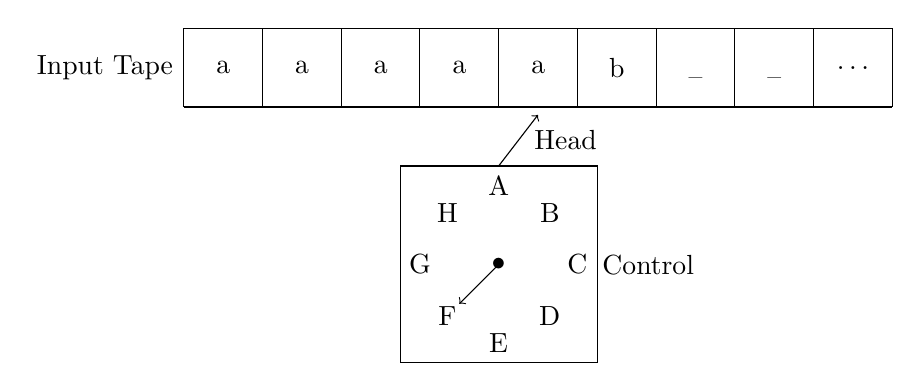
\begin{tikzpicture}
\draw (5,10) grid (6,11); %input tape
\draw (6,10) grid (7,11);
\draw (7,10) grid (8,11);
\draw (8,10) grid (9,11);
\draw (9,10) grid (10,11);
\draw (10,10) grid (11,11);
\draw (11,10) grid (12,11);
\draw (12,10) grid (13,11);
\draw (13,10) grid (14,11);
\draw (5.5,10.5) node {a}; %tape contents
\draw (6.5,10.5) node {a};
\draw (7.5,10.5) node {a};
\draw (8.5,10.5) node {a};
\draw (9.5,10.5) node {a};
\draw (10.5,10.5) node {b};
\draw (11.5,10.35) node {--};
\draw (12.5,10.35) node {--};
\draw (13.5,10.5) node {\dotss};
\draw (9,8) node[minimum size=2.5cm,draw] {$\bullet$}; %control
\draw (9,9) node {A};
\draw (9.65,8.65) node {B};
\draw (10,8) node {C};
\draw (9.65,7.35) node {D};
\draw (9,7) node {E};
\draw (8.35,7.35) node {F};
\draw (8,8) node {G};
\draw (8.35,8.65) node {H};
\draw[->] (9,8) -- (8.5,7.5); %control arrow
\draw[->] (9,9.25) -- (9.5,9.9); %head arrow
\draw (4,10.5) node {Input Tape};
\draw (10.9,8) node {Control};
\draw (9.85,9.58) node {Head};
\end{tikzpicture}

\begin{itemize}
\item<1-> The machine outlined above is called a \emph{finite-state automaton} (or \emph{finite-state machine})

\item<1-> A (very) restricted model of a computer

\item<1-> Only capable of accepting or rejecting words

\item<1-> Has no memory other than what exists in the processing module: it can only remember the state that it is
\end{itemize}

\end{scriptsize}
\end{frame}

\begin{frame}[fragile]
\frametitle{Deterministic Finite Automata}
%\framesubtitle{HOMEWORK}
\begin{scriptsize}
\begin{itemize}
\begin{definition}
A deterministic finite-state automaton, dfa, is a (make-dfa S \sig s F \delt{} [\quot{no-dead}])
\end{definition}

\item<1-> \delt{} is a transition function: must contain a transition, \texttt{(A a B)}, for every element in \texttt{S \texttt{$\times$} \sig}

\item<2-> The constructor automatically adds a \emph{dead state}, \texttt{ds} (denoted by the \fsm \ constant \texttt{DEAD}), and any missing transitions

\item<2-> For any missing transition the added transition moves the machine to the dead state

\item<2-> To inhibit the addition of the dead state the optional argument \texttt{\quot{}no-dead} may be given to the constructor

\end{itemize}
\end{scriptsize}
\end{frame}

\begin{frame}[fragile]
\frametitle{Deterministic Finite Automata}
%\framesubtitle{HOMEWORK}
\begin{scriptsize}
\begin{itemize}
\item<1-> A computation for a \dfa, \texttt{M}, is denoted by a list of configurations that \texttt{M} traverses to consume the input word

\item<1-> A configuration is a two-list that has the unconsumed part of the input word and the state the machine

\item<2-> A transition made (or step taken) by the machine is denoted using \step

\item<2-> \texttt{C$_i$} \step \ \texttt{C$_{j}$} is valid for \texttt{M} if and only if \texttt{M} can move from \texttt{C$_i$} to \texttt{C$_{j}$} using a single transition

\item<3-> Zero or more moves by \texttt{M} is denoted using \steps.

\item<3-> \texttt{C$_{i}$} \steps \ \texttt{C$_{j}$} is valid for \texttt{M} if and only if \texttt{M} can move from \texttt{C$_i$} to \texttt{C$_{j}$} using zero or more transitions

\item<4-> A word, \texttt{w}, is accepted by \texttt{M} if the following is a valid computation:
\begin{alltt}
     (w s) \steps (\elist q), where q\(\in\)F
\end{alltt}

\item<4-> The language accepted by \texttt{M}, \texttt{L(M)}, is the set of all strings accepted by \texttt{M}

\end{itemize}
\end{scriptsize}
\end{frame}

\begin{frame}[fragile]
\frametitle{Deterministic Finite Automata}
%\framesubtitle{HOMEWORK}
\begin{scriptsize}
\begin{itemize}
\item<1-> Selectors
\begin{description}
  \item[\texttt{\underline{(sm-states m)}}:] Returns the states of the given machine
  \item[\texttt{\underline{(sm-sigma m)}}:] Returns the alphabet of the given machine
  \item[\texttt{\underline{(sm-rules m)}}:] Returns the transition relation of the given machine
  \item[\texttt{\underline{(sm-start m)}}:] Returns the start state of the given machine
  \item[\texttt{\underline{(sm-finals m)}}:] Returns the final states of the given machine
  \item[\texttt{\underline{(sm-type m)}}:] Returns a symbol denoting the machine type
\end{description}

\item<2-> Observers
\begin{description}
  \item[\texttt{\underline{(sm-apply m w [n])}}:] Applies the given machine to the given word. It returns either \accept \ or \reject.
  \item[\texttt{\underline{(sm-showtransitions m w [n])}}:] Applies the given machine to the given word. It returns a list for the computation performed.
\end{description}

\item<3-> Testers
\begin{description}
  \item[\texttt{\underline{(sm-test m [n])}}:] Applies \texttt{m} to 100 randomly generated words and returns a list of the results. The optional natural number specifies the number of tests to perform.
  \item[\texttt{\underline{(sm-sameresult? m1 m2 w)}}:] Applies the two given machines, \texttt{m1} and \texttt{m2}, to, \texttt{w}, the given word and tests if the same result is obtained.
  \item[\texttt{\underline{(sm-testequiv? m1 m2 [n])}}:] Applies the two given machines, \texttt{m1} and \texttt{m2}, to the same 100 randomly generated words and tests if they produce the same results. If they do true is returned. Otherwise, a list of the words for which the results differ is returned. The optional natural number specifies the number of words to test.
\end{description}

\end{itemize}
\end{scriptsize}
\end{frame}

\begin{frame}[fragile]
\frametitle{Deterministic Finite Automata}
%\framesubtitle{HOMEWORK}
\begin{scriptsize}
\begin{itemize}
\item<1-> Machine Visualization
\begin{description}
  \item[\texttt{\underline{(sm-graph m)}}:] Returns a \emph{transition diagram} rendered as a directed graph for the given machine.
  \item[\texttt{\underline{(sm-visualize m ) [(s p)$^*$]) }}:] Starts the \fsm \ visualization tool for the given machine. The optional two-lists contain a state of the given machine and a predicate invariant (we will soon discuss this in more detail).
  \item[\texttt{\underline{(sm-cmpgraph m w)}}:] Returns a \emph{computation graph} rendered as a directed graph for the given machine. The graph summarizes how a word is accepted or rejected. A computation graph only contains the nodes and edges in the transition diagram used by a computation. A state outlined in crimson denotes where a computation stops.
\end{description}

\item<1-> Examples: abb-b.rkt

\end{itemize}
\end{scriptsize}
\end{frame}

\begin{frame}[fragile]
\frametitle{Deterministic Finite Automata}
%\framesubtitle{HOMEWORK}
\begin{scriptsize}
\begin{itemize}
\item<1-> Design Recipe for State Machines
\begin{enumerate}
\item Name the machine and specify alphabets
\item Write unit tests
\item Identify conditions that must be tracked as input is consumed, associate a state with each condition, and determine the start and final states.
\item Formulate the transition relation
\item Implement the machine
\item Test the machine using unit tests and random testing
\item Design, implement, and test an invariant predicate for each state
\item Prove L = L(M)
\end{enumerate}

\end{itemize}
\end{scriptsize}
\end{frame}

\begin{frame}[fragile]
\frametitle{Deterministic Finite Automata}
%\framesubtitle{HOMEWORK}
\begin{scriptsize}
\begin{itemize}
\item<1->
\begin{alltt}
   L = \{w | w\(\in\)\{a b\}\(\sp{*}\) \(\wedge\) w has an even number of a
                       and an odd number of b\}
\end{alltt}

\item<2->
\begin{alltt}
     ;; Name: EVEN-A-ODD-B
     ;;
     ;; \(\Sigma\): \quot{}(a b)
\end{alltt}

\item<3->
\begin{alltt}
     ;; Tests for EVEN-A-ODD-B
     #:accepts \quot{}((b) (a a b) (a a a b a b b))
     #:rejects \quot{}(() (a b b a) (b a b b a a) (a b) 
                 (a b b b b) (b a b b a a b))
\end{alltt}

\end{itemize}
\end{scriptsize}
\end{frame}

\begin{frame}[fragile]
\frametitle{Deterministic Finite Automata}
%\framesubtitle{HOMEWORK}
\begin{scriptsize}
\begin{itemize}
\item<1-> States

\item<1-> As a word is processed the consumed input may contain:
\begin{enumerate}
  \item an even number of a and an even number of b
  \item an odd number of a and an odd number of b
  \item an even number of a and an odd number of b
  \item odd number of a and even number of b
\end{enumerate}

\item<2-> When processing starts the consumed input has an even number of \texttt{a}s and an even number of \texttt{b}s

\item<3-> The state that represents that the consumed input has an even number of \texttt{a}s and an odd number of \texttt{b}s must be the only final state.

\item<4-> The states may be documented as follows:
\begin{alltt}
     ;; States
     ;; S: even number of a and even number of b, start state
     ;; M: odd number of a and odd number of b
     ;; N: even number of a and odd number of b, final state
     ;; P: odd number of a and even number of b
\end{alltt}

\end{itemize}
\end{scriptsize}
\end{frame}

\begin{frame}[fragile]
\frametitle{Deterministic Finite Automata}
%\framesubtitle{HOMEWORK}
\begin{scriptsize}
\begin{itemize}
\item<1-> Transition Function

\item<1->
\begin{alltt}
     (S a P)     \textcolor{blue}{from even-even to odd-even}
     (S b N)     \textcolor{blue}{from even-even to even-odd}
\end{alltt}

\item<2->
\begin{alltt}
     (M a N)     \textcolor{blue}{from odd-odd to even-odd}
     (M b P)     \textcolor{blue}{from odd-odd to odd-even}
\end{alltt}

\item<3->
\begin{alltt}
     (N a M)     \textcolor{blue}{from even-odd to odd-even}
     (N b S)     \textcolor{blue}{from even-odd to even-even}
\end{alltt}

\item<4->
\begin{alltt}
     (P a S)     \textcolor{blue}{from odd-even to even-even}
     (P b M)     \textcolor{blue}{from odd-even to odd-even}
\end{alltt}

\end{itemize}
\end{scriptsize}
\end{frame}

\begin{frame}[fragile]
\frametitle{Deterministic Finite Automata}
%\framesubtitle{HOMEWORK}
\begin{scriptsize}
\begin{itemize}
\item<1-> Implementation
\begin{alltt}
(define EVEN-A-ODD-B 
(make-dfa \quot{}(S M N P)
          \quot{}(a b)
          \quot{}S
          \quot{}(N)
          \quot{}((S a P) (S b N)
                  (M a N) (M b P)
                  (N a M) (N b S)
                  (P a S) (P b M))
          \quot{}no-dead
          #:accepts \quot{}((b) (a a b) (a a a b a b b))
          #:rejects \quot{}(() (a b b a) (b a b b a a) (a b) 
                      (a b b b b) (b a b b a a b))))
\end{alltt}

\item<2->
\begin{alltt}
     > (sm-test EVEN-A-ODD-B 20)
     \quot{}(((b a a a) reject)
       ((a a b a a b b) accept)
       ((b b a) reject)
       ((a b a) accept)
       (() reject)
       ((a a a a) reject)
       ((b b b a a b b) accept)
       ((b b b a b a b) accept)
            \vdotss
\end{alltt}

\end{itemize}
\end{scriptsize}
\end{frame}

\begin{frame}[fragile]
\frametitle{Deterministic Finite Automata}
%\framesubtitle{HOMEWORK}
\begin{scriptsize}
\begin{itemize}
\item<1-> You can always use \texttt{check-equal?}

\item<1-> \texttt{\#:accepts} list of words that ought to be accepted

\item<1-> \texttt{\#:rejects} list of words that ought to be rejected

\item<1-> \textcolor{red}{\textbf{Warning}}: machine is not built if expected behavior for any word is not met (unlike using check-equal?)

\end{itemize}
\end{scriptsize}
\end{frame}

\begin{frame}[fragile]
\frametitle{Deterministic Finite Automata}
%\framesubtitle{HOMEWORK}
\begin{scriptsize}
\begin{itemize}
\item<1-> State Invariants

\item<1->
\begin{alltt}
     ;; word \arrow Boolean
     ;; Purpose: Determine if given word has an even number
     ;;          of a and an even number of b
     (define (S-INV ci)
       (and (even? (length (filter (\lamb (s) (eq? s \quot{}a)) ci)))
            (even? (length (filter (\lamb (s) (eq? s \quot{}b)) ci)))))
     ;; Tests for S-INV
     (check-equal? (S-INV \quot{}(a)) #f)
     (check-equal? (S-INV \quot{}(a b b b a)) #f)
     (check-equal? (S-INV \elist) #t)
     (check-equal? (S-INV \quot{}(a a b b)) #t)
\end{alltt}

\item<2->
\begin{alltt}
     ;; word \arrow Boolean
     ;; Purpose: Determine if given word has an odd number
     ;;          of a and an odd number of b
     (define (M-INV ci)
       (and (odd? (length (filter (\lamb (s) (eq? s \quot{}a)) ci)))
            (odd? (length (filter (\lamb (s) (eq? s \quot{}b)) ci)))))
     ;; Tests for M-INV
     (check-equal? (M-INV \quot{}(a)) #f)
     (check-equal? (M-INV \quot{}(a b b b a)) #f)
     (check-equal? (M-INV \quot{}(a b b b a a b)) #f)
     (check-equal? (M-INV \quot{}(b a)) #t)
     (check-equal? (M-INV \quot{}(b a a b a b)) #t)
\end{alltt}

\end{itemize}
\end{scriptsize}
\end{frame}

\begin{frame}[fragile]
\frametitle{Deterministic Finite Automata}
%\framesubtitle{HOMEWORK}
\begin{scriptsize}
\begin{itemize}
\item<1->
\begin{alltt}
     ;; word \arrow Boolean
     ;; Purpose: Determine if given word has an even number
     ;;          of a and an odd number of b
     (define (N-INV ci)
       (and (even? (length (filter (\lamb (s) (eq? s \quot{}a)) ci)))
            (odd? (length (filter (\lamb (s) (eq? s \quot{}b)) ci)))))
     ;; Tests for N-INV
     (check-equal? (N-INV \elist) #f)
     (check-equal? (N-INV \quot{}(a b a b a)) #f)
     (check-equal? (N-INV \quot{}(a b b a a b)) #f)
     (check-equal? (N-INV \quot{}(b a a)) #t)
     (check-equal? (N-INV \quot{}(a b a a b a b b b)) #t)
\end{alltt}

\item<2->
\begin{alltt}
     ;; word \arrow Boolean
     ;; Purpose: Determine if given word has an odd number
     ;;          of a and an even number of b
     (define (P-INV ci)
       (and (odd? (length (filter (\lamb (s) (eq? s \quot{}a)) ci)))
            (even? (length (filter (\lamb (s) (eq? s \quot{}b)) ci)))))
     ;; Tests for P-INV
     (check-equal? (P-INV \elist) #f)
     (check-equal? (P-INV \quot{}(a b)) #f)
     (check-equal? (P-INV \quot{}(a b b a a b a)) #f)
     (check-equal? (P-INV \quot{}(b a b)) #t)
     (check-equal? (P-INV \quot{}(a b a a b b b)) #t)
\end{alltt}

\end{itemize}
\end{scriptsize}
\end{frame}

\begin{frame}[fragile]
\frametitle{Deterministic Finite Automata}
%\framesubtitle{HOMEWORK}
\begin{scriptsize}
\begin{itemize}
\item<1-> Validate invariants using \texttt{sm-visualize}

\item<2-> For the required proofs we use the following notation:
\begin{alltt}
     M = EVEN-A-ODD-B
     \(\sig\) = (sm-sigma M)
     F = (sm-finals M)
     w \(\in\) \(\sig\sp{*}\)
     ci = the consumed input
\end{alltt}

\end{itemize}
\end{scriptsize}
\end{frame}

\begin{frame}[fragile]
\frametitle{Deterministic Finite Automata}
%\framesubtitle{HOMEWORK}
\begin{scriptsize}

\begin{theorem}
The state invariants hold when M is applied to w.
\end{theorem}

\begin{itemize}

\item<1-> Proof by induction on the number of transitions, n, M makes to consume w.

\item<2-> \underline{Base Case}: n = 0\\
If n is 0 then the consumed input is \elist{} and M is in S. This means the consumed input has an even number of \texttt{a}s and an even number of \texttt{b}s (0 of each). Therefore, S-INV holds.\\

\item<3-> \underline{Inductive Step}:\\
Assume: State invariants hold for n = k.\\
Show: State invariants hold for n = k+1.\\

\item<4-> If n=k+1 then the consumed input cannot be \elist{} given that the machine must have consumed at least one symbol. Therefore, we can state that ci=xa such that $|$ci$|$=k+1, x$\in$\sig$^*$ and a$\in$\sig. M's computation to consume ci has k+1 steps: \\
\begin{center}
     (xa s) \step$^{k}$ (a r) \step \ (\elist \ q), where r,q$\in$S
\end{center}

\item<4-> Given that $|$x$|$=k the inductive hypothesis informs us that the state invariants hold when x is consumed by M

\item<5-> We must show that the state invariants hold for the k+1 transition into q

\end{itemize}
\end{scriptsize}
\end{frame}

\begin{frame}[fragile]
\frametitle{Deterministic Finite Automata}
%\framesubtitle{HOMEWORK}
\begin{scriptsize}
\begin{itemize}
\item<1-> \underline{\texttt{(S a P)}}: Assume S-INV holds. Consuming an \texttt{a} means ci has an odd number of \texttt{a}s and an even number \texttt{b}s. Therefore, P-INV holds. \\

\item<2-> \underline{\texttt{(S b N)}}: Assume S-INV holds. Consuming a \texttt{b} means ci has an even number of \texttt{a}s and an odd number \texttt{b}s. Therefore, N-INV holds. \\

\item<3->  \underline{\texttt{(M a N)}}: Assume M-INV holds. Consuming an \texttt{a} means ci has an even number of \texttt{a}s and an odd number \texttt{b}s. Therefore, N-INV holds. \\

\item<4-> \underline{\texttt{(M b P)}}:  Assume M-INV holds. Consuming an \texttt{b} means ci has an odd number of \texttt{a}s and an even number \texttt{b}s. Therefore, P-INV holds.\\

\item<5-> \underline{\texttt{(N a M)}}:  Assume N-INV holds. Consuming an \texttt{a} means ci has an odd number of \texttt{a}s and an odd number \texttt{b}s. Therefore, M-INV holds.\\

\item<6-> \underline{\texttt{(N b S)}}:  Assume N-INV holds. Consuming an \texttt{b} means ci has an even number of \texttt{a}s and an even number \texttt{b}s. Therefore, S-INV holds.\\

\item<7-> \underline{\texttt{(P a S)}}:  Assume P-INV holds. Consuming an \texttt{a} means ci has an even number of \texttt{a}s and an even number \texttt{b}s. Therefore, S-INV holds.\\

\item<8-> \underline{\texttt{(P b M)}}:  Assume P-INV holds. Consuming an \texttt{b} means ci has an odd number of \texttt{a}s and an odd number \texttt{b}s. Therefore, M-INV holds

\end{itemize}
\end{scriptsize}
\end{frame}

\begin{frame}[fragile]
\frametitle{Deterministic Finite Automata}
%\framesubtitle{HOMEWORK}
\begin{scriptsize}
\begin{itemize}
\item<1-> The proof that \texttt{L(EVEN-A-ODD-B) = L} is divided into two lemmas (i.e., two parts):
\begin{enumerate}
  \item w\(\in\)L \(\Leftrightarrow\) w\(\in\)L(M)
  \item w\(\notin\)L \(\Leftrightarrow\) w\(\notin\)L(M)
\end{enumerate}

\end{itemize}
\end{scriptsize}
\end{frame}

\begin{frame}[fragile]
\frametitle{Deterministic Finite Automata}
%\framesubtitle{HOMEWORK}
\begin{scriptsize}
\begin{lemma}
     w\(\in\)L \(\Leftrightarrow\) w\(\in\)L(M)
\end{lemma}

\begin{itemize}
\item<1-> ($\Rightarrow$) Assume w\(\in\)L.\\

w\(\in\)L  means that w has an even number of \texttt{a}s and an odd number of \texttt{b}s. The proof that state invariants hold when w is consumed means that M can only halt in N, which is a final state. Therefore, w$\in$L(M).

\item<2-> ($\Leftarrow$) Assume w\(\in\)L(M).\\

\noindent w\(\in\)L(M) means that M halts in N. N's invariant guarantees that w has an even number of \texttt{a}s and an odd number of \texttt{b}s. Therefore, w\(\in\)L.

\end{itemize}
\end{scriptsize}
\end{frame}

\begin{frame}[fragile]
\frametitle{Deterministic Finite Automata}
%\framesubtitle{HOMEWORK}
\begin{scriptsize}
\begin{lemma}
     w\(\notin\)L \(\Leftrightarrow\) w\(\notin\)L(M)
\end{lemma}

\begin{itemize}
\item<1-> ($\Rightarrow$) Assume w\(\notin\)L.\\

w\(\notin\)L means that w does not have an even number of \texttt{a}s and an odd number of \texttt{b}s. This means M does not halt in N after consuming w. Given that the state invariants always hold, this means that w$\notin$L(M).

\item<2-> ($\Leftarrow$) Assume w\(\notin\)L(M).\\

M does not halt in N (the only final state). Given that the state invariants always hold, this means that w does not have an even number of \texttt{a}s and an odd number of \texttt{b}s. Therefore, w\(\notin\)L.

\end{itemize}
\end{scriptsize}
\end{frame}

\begin{frame}[fragile]
\frametitle{Deterministic Finite Automata}
%\framesubtitle{HOMEWORK}
\begin{scriptsize}
\begin{theorem}
L = L(EVEN-A-ODD-B)
\end{theorem}

\begin{itemize}
\item<1-> The two previous lemmas establish the theorem.

\end{itemize}
\end{scriptsize}
\end{frame}

\begin{frame}[fragile]
\frametitle{Deterministic Finite Automata}
%\framesubtitle{HOMEWORK}
\begin{scriptsize}
\begin{itemize}
\item<1-> HOMEWORK: 1, 2, 4, 5, 7, 12

\item<1-> QUIZ: 10 (due in 1 week)

\end{itemize}
\end{scriptsize}
\end{frame}

\begin{frame}[fragile]
\frametitle{Deterministic Finite Automata}
%\framesubtitle{HOMEWORK}
\begin{scriptsize}
\begin{itemize}
\item<1-> Pattern Detection (i.e., \texttt{Ctrl-F})

\item<2-> Given a pattern, \texttt{patt}, and an alphabet, \texttt{sigma}, the \dfa{} built needs \texttt{$|$patt$|$+1} states

\item<2-> These states form the \dfa{}'s backbone and lead from the starting to the final state consuming the pattern

\item<3-> The \dfa{} backbone for the pattern \texttt{\quot{}(a b b a b c)} has the following structure:
\begin{center}
\includegraphics[scale=0.4]{dfa-backbone.png}
\end{center}

\item<3-> Not the complete \dfa{} because it is missing the transitions for when the next symbol in a given word does not match the next symbol in the pattern

\item<3-> If the machine is in state \texttt{E} and the next symbol in the input word is not \texttt{c}, what state should the machine move to?

\end{itemize}
\end{scriptsize}
\end{frame}

\begin{frame}[fragile]
\frametitle{Deterministic Finite Automata}
%\framesubtitle{HOMEWORK}
\begin{scriptsize}
\begin{center}
\includegraphics[scale=0.4]{dfa-backbone.png}
\end{center}

\begin{itemize}
\item<1-> Reason about what the states mean (i.e., their invariant properties). For the machine's backbone above we can state:
\begin{description}
  \item[\underline{\texttt{S}}] Nothing in the pattern has been matched
  \item[\underline{\texttt{A}}] a has been matched
  \item[\underline{\texttt{B}}] ab has been matched
  \item[\underline{\texttt{C}}] abb has been matched
  \item[\underline{\texttt{D}}] abba has been matched
  \item[\underline{\texttt{E}}] abbab has been matched
  \item[\underline{\texttt{F}}] abbabc has been matched
\end{description}

\item<2-> What state should the machine be in after reading \texttt{\quot{}(a b b a b b)}?

\item<3-> Observe that longest suffix of the read input that matches the beginning of the pattern is \texttt{\quot{}(a b b)}

\item<3-> The machine needs to move to state \texttt{C}.

\end{itemize}
\end{scriptsize}
\end{frame}

\begin{frame}[fragile]
\frametitle{Deterministic Finite Automata}
%\framesubtitle{HOMEWORK}
\begin{scriptsize}

\begin{center}
\includegraphics[scale=0.4]{dfa-backbone.png}
\end{center}

\begin{itemize}
\item<1-> How are the transition rules computed for when the next input symbol does not match the next symbol in the pattern?

\item<1-> We say that the part of the pattern matched for each state represents the core prefix of the state

\item<1-> For \texttt{B} the core prefix is \texttt{\quot{}(a b)}

\item<1-> For \texttt{E} the core prefix is \texttt{\quot{}(a b b a b)}

\end{itemize}
\end{scriptsize}
\end{frame}

\begin{frame}[fragile]
\frametitle{Deterministic Finite Automata}
%\framesubtitle{HOMEWORK}
\begin{scriptsize}
\begin{center}
\includegraphics[scale=0.4]{dfa-backbone.png}
\end{center}

\begin{itemize}
\item<1-> We use core prefixes to compute the transitions needed for each state

\item<2-> Assume the states are kept in a list such that the states appear in the direction of the arrows: \texttt{states = \quot{}(S A B C D E F)}

\item<3-> What are the needed transitions out of \texttt{E}?

\item<4-> \texttt{E}'s core prefix is \texttt{\quot{}(a b b a b)}

\item<4-> The next input symbol may be \texttt{a}, \texttt{b}, or \texttt{c}

\item<4-> For each, identify longest suffix that matches the pattern's beginning

\item<5-> For \texttt{a} we have:
\begin{alltt}
     Last 6 symbols of consumed input: \texttt{\quot{}(a b b a b a)}
\end{alltt}

\item<6-> Compare successively shorter suffixes with the pattern's beginning until a match is found or the suffix is empty:
\begin{alltt}
      Pattern: \quot{}(a b b a b c)
       Suffix: \quot{}(a b b a b a) \(\rightarrow\) does not match
               \quot{}(b b a b a)   \(\rightarrow\) does not match
               \quot{}(b a b a)     \(\rightarrow\) does not match
               \quot{}(a b a)       \(\rightarrow\) does not match
               \quot{}(b a)         \(\rightarrow\) does not match
               \quot{}(a)           \(\rightarrow\) match
\end{alltt}

\item<6-> The longest matching suffix with the pattern's beginning is \texttt{A}'s core prefix

\item<6-> This means that the machine must transition to \texttt{A}: \texttt{(E a A)}

\end{itemize}
\end{scriptsize}
\end{frame}

\begin{frame}[fragile]
\frametitle{Deterministic Finite Automata}
%\framesubtitle{HOMEWORK}
\begin{scriptsize}
\begin{center}
\includegraphics[scale=0.4]{dfa-backbone.png}
\end{center}


\begin{itemize}
\item<1-> For \texttt{b}:
\begin{alltt}
      Pattern: \quot{}(a b b a b c)
       Suffix: \quot{}(a b b a b b) \(\rightarrow\) does not match
               \quot{}(b b a b b)   \(\rightarrow\) does not match
               \quot{}(b a b b)     \(\rightarrow\) does not match
               \quot{}(a b b)       \(\rightarrow\) match
\end{alltt}

\item<1-> The longest matching suffix with the pattern's beginning is \texttt{C}'s core prefix

\item<1-> The machine needs to transition to \texttt{C}: \texttt{(E b C)}

\item<2-> For \texttt{c}:
\begin{alltt}
      Pattern: \quot{}(a b b a b c)
       Suffix: \quot{}(a b b a b c) \(\rightarrow\) match
\end{alltt}

\item<2-> The longest matching suffix with the pattern's beginning is \texttt{F}'s core prefix

\item<2-> The needed transition is \texttt{(E c F)}

\end{itemize}
\end{scriptsize}
\end{frame}

\begin{frame}[fragile]
\frametitle{Deterministic Finite Automata}
%\framesubtitle{HOMEWORK}
\begin{scriptsize}
\begin{itemize}
\item<1-> \texttt{states = \quot{}(S A B C D E F)}

\item<1-> Have you noticed the pattern for the destination state in each of the computed transition rules?

\item<2-> It is always \texttt{(list-ref states (length lsuffix))}, where \texttt{lsuffix} is the longest matching suffix

\item<2->
\begin{alltt}
     (list-ref states (length \quot{}(a))) = A
     (list-ref states (length \quot{}(a b b))) = C
     (list-ref states (length \quot{}(a b b a b c))) = F
\end{alltt}

\end{itemize}
\end{scriptsize}
\end{frame}




\begin{frame}[fragile]
\frametitle{Deterministic Finite Automata}
%\framesubtitle{HOMEWORK}
\begin{scriptsize}
\begin{itemize}
\item<1-> For a given pattern, \texttt{patt}, and a given input alphabet, \texttt{sigma}, the goal is to build a \dfa{} for the following language:
\begin{alltt}
     L = \{w | w contains patt\}
\end{alltt}

\item<2-> The constructor needs to:
\begin{enumerate}
  \item Generate the states for the new \dfa
  \item Compute the core prefix for each state
  \item Compute the transitions for the new \dfa
\end{enumerate}


\item<3-> We choose to define the first state in the list of generated states as the starting state and the last state generated as the final state

\item<3-> To generate a state the \fsm{} function \texttt{gen-state} is used
\begin{alltt}
(gen-state l) → state
  l : (listof state)
Generates a state not in the given list of states.
\end{alltt}

\item<4-> The generation of the core prefixes may be done so as to correspond with the list of generated states.

\item<4-> The core prefix for the \texttt{i$^{\texttt{ith}}$} state is given by taking the first \texttt{i} elements of the pattern.

\item<5-> To generate the transition function the needed transitions for each state, \texttt{s}, may be generated using the states, the input alphabet, the core prefix for \texttt{s}, and the pattern

\end{itemize}
\end{scriptsize}
\end{frame}

\begin{frame}[fragile]
\frametitle{Deterministic Finite Automata}
%\framesubtitle{HOMEWORK}
\begin{tiny}
\begin{itemize}
\item<1->
\begin{alltt}
;; word alphabet \arrow dfa
;; Purpose: Build a dfa for L = all words that contain the
;;                              given pattern
(define (build-pattern-dfa patt sigma)
\end{alltt}

\item<3->
\begin{alltt}
  (let* [(sts (foldl (\lamb{} (s acc) (cons (gen-state acc) acc))
                     \elist{}
                     (cons 1 patt))) ;; number of states = |patt|+1
\end{alltt}

\item<4->
\begin{alltt}
         (core-prefixes (build-list (add1 (length patt))
                                    (\lamb (i) (take patt i))))
\end{alltt}

\item<5->
\begin{alltt}
         (deltas (append-map
                   (\lamb (s cp)
                     (gen-state-trans s sts sigma cp patt))
                   sts
                   core-prefixes))]
\end{alltt}

\item<6->
\begin{alltt}
    (make-dfa sts sigma (first sts) (list (last sts)) deltas \quot{}no-dead)))
\end{alltt}

\item<2->
\begin{alltt}
     ;; Tests for build-pattern-dfa \textbf{\textcolor{red}{YUCK!}}
     (define M (build-pattern-dfa \quot{}(a b b a) \quot{}(a b)))
     (define N (build-pattern-dfa \quot{}(a d) \quot{}(a b c d)))

     (check-equal? (sm-apply M \elist) \quot{}reject)
     (check-equal? (sm-apply M \quot{}(a a b b b a)) \quot{}reject)
     (check-equal? (sm-apply M \quot{}(b b b a a a b b)) \quot{}reject)
     (check-equal? (sm-apply M \quot{}(a b b a)) \quot{}accept)
     (check-equal? (sm-apply M \quot{}(b b a a a b b a b b a)) \quot{}accept)
     (check-equal? (sm-apply M \quot{}(a b b b a b b a)) \quot{}accept)

     (check-equal? (sm-apply N \elist) \quot{}reject)
     (check-equal? (sm-apply N \quot{}(a b c d a b c c)) \quot{}reject)
     (check-equal? (sm-apply N \quot{}(c c b a b d)) \quot{}reject)
     (check-equal? (sm-apply N \quot{}(a d)) \quot{}accept)
     (check-equal? (sm-apply N '(b c a a d c c b)) 'accept)
     (check-equal? (sm-apply N '(c d b c a d c a d)) 'accept)
\end{alltt}

\end{itemize}
\end{tiny}
\end{frame}

\begin{frame}[fragile]
\frametitle{Deterministic Finite Automata}
%\framesubtitle{HOMEWORK}
\begin{tiny}
\begin{itemize}
\item<1->
\begin{alltt}
;; word alphabet \arrow dfa
;; Purpose: Build a dfa for L = all words that contain the
;;                              given pattern
(define (build-pattern-dfa patt sigma)
\end{alltt}

\item<1->
\begin{alltt}
  (let* [(sts (foldl (\lamb{} (s acc) (cons (gen-state acc) acc))
                     \elist{}
                     (cons 1 patt))) ;; number of states = |patt|+1
\end{alltt}

\item<1->
\begin{alltt}
         (core-prefixes (build-list (add1 (length patt))
                                    (\lamb (i) (take patt i))))
\end{alltt}

\item<1->
\begin{alltt}
         (deltas (append-map
                   (\lamb (s cp)
                     (gen-state-trans s sts sigma cp patt))
                   sts
                   core-prefixes))]
\end{alltt}

\item<1->
\begin{alltt}
    (make-dfa sts sigma (first sts) (list (last sts)) deltas \quot{}no-dead)))
\end{alltt}

\item<1->
\begin{alltt}
     ;; Tests for build-pattern-dfa \textbf{\textcolor{darkgreen}{Poetry!}}
     (define M (build-pattern-dfa \quot{}(a b b a) \quot{}(a b)))
     (define N (build-pattern-dfa \quot{}(a d) \quot{}(a b c d)))

     (check-reject? M \quot{}() \quot{}(a a b b b a) \quot{}(b b b a a a b b))
     (check-accept? M \quot{}(a b b a) \quot{}(b b a a a b b a b b a) \quot{}(a b b b a b b a))

     (check-reject? N \quot{}() \quot{}(a b c d a b c c) \quot{}(c c b a b d))
     (check-accept? N \quot{}(a d) \quot{}(b c a a d c c b) \quot{}(c d b c a d c a d))

\end{alltt}

\end{itemize}
\end{tiny}
\end{frame}

\begin{frame}[fragile]
\frametitle{Deterministic Finite Automata}
%\framesubtitle{HOMEWORK}
\begin{scriptsize}
\begin{itemize}
\item<1->
\begin{alltt}
;; state (listof state) alphabet word word \arrow (listof dfa-rule)
;; Purpose: Generate failed match transitions for the
;;          given state
(define (gen-state-trans s states sigma cp patt)
\end{alltt}

\item<3->
\begin{alltt}
  (map (\lamb (a)
         (gen-state-tran s (append cp (list a)) patt states a))
       sigma))
\end{alltt}

\item<2->
\begin{alltt}
;; Tests for gen-state-trans
(check-equal?
  (gen-state-trans \quot{}E
                   \quot{}(S A B C D E F)
                   \quot{}(a b c)
                   \quot{}(a b b a b)
                   \quot{}(a b b a b c))
  \quot{}((E a A) (E b C) (E c F)))

(check-equal?
  (gen-state-trans \quot{}S
                   \quot{}(S A B C D E F)
                   \quot{}(a b c)
                   \quot{}()
                   \quot{}(a b b a b c))
  \quot{}((S a A) (S b S) (S c S)))
     \vdotss{}
\end{alltt}

\end{itemize}
\end{scriptsize}
\end{frame}

\begin{frame}[fragile]
\frametitle{Deterministic Finite Automata}
%\framesubtitle{HOMEWORK}
\begin{scriptsize}
\begin{itemize}
\item<1->
\begin{alltt}
;; state word word (listof state) symbol \arrow dfa-rule
;; Purpose: Generate dfa rule for given state and given word
;;          to match in the given pattern
(define (gen-state-tran s to-match patt states last-read)
\end{alltt}

\item<3->
\begin{alltt}
  (cond [(empty? to-match) (list s last-read (first states))]
\end{alltt}

\item<4->
\begin{alltt}
        [(> (length to-match) (length patt))
         (list s last-read s)]
\end{alltt}

\item<5->
\begin{alltt}
        [(equal? to-match (take patt (length to-match)))
         (list s
               (last to-match)
               (list-ref states (length to-match)))]
\end{alltt}

\item<6->
\begin{alltt}
        [else (gen-state-tran s
                              (rest to-match)
                              patt
                              states
                              last-read)]))
\end{alltt}

\item<2->
\begin{alltt}
;; Tests for gen-state-tran
(check-equal?
  (gen-state-tran
    \quot{}C \quot{}(a b b b) \quot{}(a b b a b c) \quot{}(S A B C D E F) \quot{}b)
  \quot{}(C b S))
(check-equal?
  (gen-state-tran
    \quot{}S \quot{}(b) \quot{}(a b b a b c) \quot{}(S A B C D E F) \quot{}b)
  \quot{}(S b S))  \dotss{}
\end{alltt}

\end{itemize}
\end{scriptsize}
\end{frame}

\begin{frame}[fragile]
\frametitle{Deterministic Finite Automata}
%\framesubtitle{HOMEWORK}
\begin{scriptsize}
\begin{itemize}
\item<1-> This algorithm is the basis for the efficient and widely implemented Knuth-Morris-Pratt (\texttt{KMP}) algorithm

\item<1-> The \texttt{KMP} algorithm is a string matching algorithm that looks for occurrences of a string in a block of text

\item<2-> Given that most programming languages do not have a \dfa{} type like \fsm{}, the KMP algorithm represents the \dfa{} differently

\item<2-> It uses a vector of indices into the pattern to represent where matching ought to continue when the next element in the text does not match the next element in the pattern

\item<2-> You are strongly encourage to review the \texttt{KMP} algorithm.

\end{itemize}
\end{scriptsize}
\end{frame}

\begin{frame}[fragile]
\frametitle{Deterministic Finite Automata}
%\framesubtitle{HOMEWORK}
\begin{scriptsize}
\begin{itemize}
\item<1-> HOMEWORK: 19

\item<1-> Quiz: 20 (due in 1 week)

\end{itemize}
\end{scriptsize}
\end{frame}





\section{Nondeterministic Finite Automata}

\begin{frame}[fragile]
\frametitle{Nondeterministic Finite Automata}
%\framesubtitle{HOMEWORK}
\begin{scriptsize}
\begin{itemize}
\item<1-> \dfa{} can decide a language whose words are built using concatenation and Kleene star

\item<2->
\begin{center}
\includegraphics[scale=0.3]{sample-concat-star-dfa.png}
\end{center}

\item<2-> A transition in a \dfa{} represents concatenating an alphabet symbol

\item<2-> A loop is concatenating a value generated by a Kleene star--the loop may be entered 0 or more times

\item<3-> What about deciding a regular language that requires union?

\item<4->
\begin{alltt}
     L = ab\(\sp{*}\) \(\cup\) aa\(\sp{*}\) \(\cup\) \(\epsilon\)
\end{alltt}

\item<4-> There are three types of words that may be generated.

\item<4-> It is not difficult to build a \dfa{} for the language represented by each regular expression choice in the union:
\begin{center}
\includegraphics[scale=0.3]{union-choices.png}
\end{center}

\item<4-> It is difficult, however, to see how \texttt{L} can be decided by a \dfa{}

\end{itemize}
\end{scriptsize}
\end{frame}

\begin{frame}[fragile]
\frametitle{Nondeterministic Finite Automata}
%\framesubtitle{HOMEWORK}
\begin{scriptsize}
\begin{itemize}
\item<1-> A new model of a computer is needed

\item<1-> One that allows a machine to change state in a manner that is not fully determined by the transition relation

\item<1-> When the machine has a choice it nondeterministically chooses which transition (or transitions) to use

\item<2-> For instance, consider a finite-state machine for \texttt{L}:
\begin{center}
\includegraphics[scale=0.35]{ndfa-L.png}
\end{center}

\end{itemize}
\end{scriptsize}
\end{frame}

\begin{frame}[fragile]
\frametitle{Nondeterministic Finite Automata}
%\framesubtitle{HOMEWORK}
\begin{scriptsize}
\begin{center}
\includegraphics[scale=0.15]{ndfa-L.png}
\end{center}

\begin{itemize}
\item<1-> Two new characteristics:
\begin{itemize}
  \item \begin{scriptsize} May change state without consuming anything \end{scriptsize}
  \item \begin{scriptsize} From a given state there may be more than one transition \end{scriptsize}
\end{itemize}

\item<1-> The transition relation is not a function

\item<1-> Given the same input the machine may carry out different computations

\item<2-> Processing \texttt{\quot{}(a b b)}:
\begin{alltt}
     ((a b b) S) \step ((a b b) F)
     ((a b b) S) \step ((b b) B)
     ((a b b) S) \step ((b b) A) \step ((b) A) \step (() A)
\end{alltt}

\item<2-> The first two computations reject because input not consumed

\item<2-> The third computation accepts \texttt{\quot{}(a b b)}

\item<2-> Based on this, is \texttt{\quot{}(a b b)} in \texttt{L} or not?

\item<3-> A word is in the language of a nondeterministic finite-state machine if there is at least one computation that leads to accept

\item<4-> You may assume that if the input word is in the machine's language then every nondeterministic choice made during a computation is part of a computation that leads to the machine accepting the word

\item<4-> Machines with such ``intuition'' sound very powerful, no?

\end{itemize}
\end{scriptsize}
\end{frame}

\begin{frame}[fragile]
\frametitle{Nondeterministic Finite Automata}
%\framesubtitle{HOMEWORK}
\begin{scriptsize}
\begin{itemize}
\begin{definition}
A nondeterministic finite-state automaton, ndfa, is a (make-ndfa K \sig S F \delt)
\end{definition}

\item<1-> \delt{} is a transition relation, not a function, that may have \ets{} and multiple transitions from a state on the same alphabet element

\item<2-> An \ndfa{} (transition) rule is defined as follows:
\begin{alltt}
     (Q a R), where Q,R\(\in\)K \(\wedge\) a\(\in\)\{\(\sig\cup\{\epsilon\}\)\}
\end{alltt}

\item<3-> Given a configuration \texttt{(m r)}, where \texttt{m$\in\sig^{\texttt{*}}$} and \texttt{r$\in$K}, the machine may have no transitions it may follow and halts or may move to one of several different configurations because of \ets{} or multiple transitions from \texttt{r} on the same alphabet element

\item<4-> A word, \texttt{w}, is accepted by an \ndfa, \texttt{N}, if there exists a computation such that:
\begin{alltt}
     (w s) \steps (() f), where f\(\in\)F
\end{alltt}

\item<4-> The language of \texttt{N}, \texttt{L(N)}, is all the words accepted by \texttt{N}.

\item<5-> Every \dfa{} is an \ndfa{}

\end{itemize}
\end{scriptsize}
\end{frame}

\begin{frame}[fragile]
\frametitle{Nondeterministic Finite Automata}
%\framesubtitle{HOMEWORK}
\begin{scriptsize}
\begin{center}
\includegraphics[scale=0.2]{ndfa-L.png}
\end{center}

\begin{itemize}
\item<1->
\begin{alltt}
#lang fsm
;; L = \{\(\epsilon\)\} \(\cup\) aa* \(\cup\) ab*
(define LNDFA 
  (make-ndfa \quot{}(S A B F)
\end{alltt}

\item<3->
\begin{alltt}
             \quot{}(a b)
\end{alltt}

\item<4->
\begin{alltt}
             \quot{}S
\end{alltt}

\item<5->
\begin{alltt}
             \quot{}(A B F)
\end{alltt}

\item<6->
\begin{alltt}
             \qquot{}((S a A) (S a B) (S ,EMP F)
               (A b A) (B a B))
\end{alltt}

\item<2->
\begin{alltt}
             #:rejects \quot{}((a b a) (b b b b b) (a b b b b a a a))
             #:accepts \quot{}(() (a) (a a a a) (a b b))))
\end{alltt}

\item<6-> The only transitions listed are those that are on a path to an accepting state

\end{itemize}
\end{scriptsize}
\end{frame}

\begin{frame}[fragile]
\frametitle{Nondeterministic Finite Automata}
%\framesubtitle{HOMEWORK}
\begin{scriptsize}
\begin{itemize}
\item<1-> Designing an \ndfa{} can prove easier than designing a \dfa{}

\item<2-> Care must be taken when reasoning about the machine:
\begin{center}
\includegraphics[scale=0.4]{empties-ndfa.png}
\end{center}

\item<2-> What state does the machine move to if it is in \texttt{S} and consumes an \texttt{a}?

\item<3-> The machine may end in \texttt{S}, \texttt{A}, or \texttt{B}

\item<3-> State invariant must hold for any state in a computation that leads to accept

\end{itemize}
\end{scriptsize}
\end{frame}

\begin{frame}[fragile]
\frametitle{Nondeterministic Finite Automata}
%\framesubtitle{HOMEWORK}
\begin{scriptsize}
\begin{itemize}
\item<1-> To aid us in reasoning about \ndfa{}s we define the \emph{empties} of a state \texttt{R}:
\begin{alltt}
     E(R) = \{\{R\} \(\cup\) \{P | ((\(\epsilon\) R) \steps (\(\epsilon\) P))\}\}
\end{alltt}

\item<1-> That is, \texttt{E(R)} contains \texttt{R} and all states reachable from \texttt{R} by only following \ets

\item<2->
\begin{center}
\includegraphics[scale=0.4]{empties-ndfa.png}
\end{center}
\begin{alltt}
     E(S) = \{S A B\}
     E(A) = \{A B\}
     E(B) = \{B\}
\end{alltt}

\end{itemize}
\end{scriptsize}
\end{frame}

\begin{frame}[fragile]
\frametitle{Nondeterministic Finite Automata}
%\framesubtitle{HOMEWORK}
\begin{scriptsize}
\begin{itemize}
\item<1->
\begin{alltt}
     L = \{w | a\(\notin\)w \(\vee\) b\(\notin\)w \(\vee\) c\(\notin\)w\}
\end{alltt}

\item<2-> Name: \texttt{AT-LEAST-ONE-MISSING}

\item<2-> \sig{} = \texttt{\{a b c\}}

\item<3->
\begin{alltt}
;; Tests for AT-LEAST-ONE-MISSING
#:rejects \quot{}((a b c) (b b a b c b a) (b a c))
#:accepts \quot{}(() (a) (b) (c) (c c a a) (b b c b b b) (a a a b b b))
\end{alltt}

\end{itemize}
\end{scriptsize}
\end{frame}

\begin{frame}[fragile]
\frametitle{Nondeterministic Finite Automata}
%\framesubtitle{HOMEWORK}
\begin{scriptsize}
\begin{itemize}
\item<1-> Design Idea and conditions

\item<1-> Nondeterministically decides to process the word as if \texttt{a} is missing, as if \texttt{b} is missing, or as if \texttt{c} is missing

\item<2-> The consumed input, \texttt{ci}, must satisfy one of four conditions: nothing is consumed or for each \texttt{x$\in$(sm-sigma AT-LEAST-ONE-MISSING)} \texttt{x$\notin$ci}

\item<3-> Four states are needed:
\begin{alltt}
     ;; States
     ;; S: the consumed input is empty, starting state
     ;; A: the consumed input does not contain a, final state
     ;; B: the consumed input does not contain b, final state
     ;; C: the consumed input does not contain c, final state
\end{alltt}

\end{itemize}
\end{scriptsize}
\end{frame}

\begin{frame}[fragile]
\frametitle{Nondeterministic Finite Automata}
%\framesubtitle{HOMEWORK}
\begin{scriptsize}
\begin{itemize}
\item<1-> Transition Relation

\item<1-> In \texttt{S} nondeterministically move to either \texttt{A}, \texttt{B}, or \texttt{C}

\item<2-> In \texttt{A} process arbitrary number of \texttt{b}s or \texttt{c}s

\item<3-> In \texttt{B} processes arbitrary number of \texttt{a}s or \texttt{c}s

\item<4-> In \texttt{C} process arbitrary number of \texttt{a}s or \texttt{b}s.

\item<1-> The transition relation is:
\begin{alltt}
     \qquot{}((S ,EMP A)
       (S ,EMP B)
       (S ,EMP C)
\end{alltt}

\item<2->
\begin{alltt}
       (A b A)
       (A c A)
\end{alltt}

\item<3->
\begin{alltt}
       (B a B)
       (B c B)
\end{alltt}

\item<4->
\begin{alltt}
       (C a C)
       (C b C))
\end{alltt}

\end{itemize}
\end{scriptsize}
\end{frame}

\begin{frame}[fragile]
\frametitle{Nondeterministic Finite Automata}
%\framesubtitle{HOMEWORK}
\begin{scriptsize}
\begin{itemize}
\item<1->
\begin{alltt}
     ;; States
     ;; S: the consumed input is empty, starting state
     ;; A: the consumed input does not contain a, final state
     ;; B: the consumed input does not contain b, final state
     ;; C: the consumed input does not contain c, final state
\end{alltt}

\item<1->
\begin{alltt}
  ;; word \arrow Boolean
  ;; Purpose: Determine if the given word is empty
  (define (S-INV ci) (empty? ci))

  ;; Test for S-INV
  (check-equal? (S-INV \elist) #t)
  (check-equal? (S-INV '(a b)) #f)
\end{alltt}

\item<2->
\begin{alltt}
  ;; word \arrow Boolean
  ;; Purpose: Determine if the given word does not contain a
  (define (A-INV ci) (empty? (filter (\lamb (a) (eq? a \quot{}a)) ci)))

  ;; Test for A-INV
  (check-equal? (A-INV \quot{}(a)) #f)
  (check-equal? (A-INV \quot{}(a c b)) #f)
  (check-equal? (A-INV \quot{}(c c b a b)) #f)
  (check-equal? (A-INV \quot{}(b)) #t)
  (check-equal? (A-INV \quot{}(c c b c b)) #t)
  (check-equal? (A-INV \elist) #t)
\end{alltt}

\end{itemize}
\end{scriptsize}
\end{frame}

\begin{frame}[fragile]
\frametitle{Nondeterministic Finite Automata}
%\framesubtitle{HOMEWORK}
\begin{scriptsize}
\begin{itemize}
\item<1->
\begin{alltt}
     ;; States
     ;; S: the consumed input is empty, starting state
     ;; A: the consumed input does not contain a, final state
     ;; B: the consumed input does not contain b, final state
     ;; C: the consumed input does not contain c, final state
\end{alltt}

\item<1->
\begin{alltt}
  ;; word \arrow Boolean
  ;; Purpose: Determine if the given word does not contain b
  (define (B-INV ci) (empty? (filter (\lamb (a) (eq? a \quot{}b)) ci)))

  ;; Test for B-INV
  (check-equal? (B-INV \quot{}(b)) #f)
  (check-equal? (B-INV \quot{}(a c b)) #f)
  (check-equal? (B-INV \quot{}(a a b a b)) #f)
  (check-equal? (B-INV \quot{}(c)) #t)
  (check-equal? (B-INV \quot{}(c c a c c a a a)) #t)
  (check-equal? (B-INV \elist) #t)
\end{alltt}

\item<2->
\begin{alltt}
  ;; word \arrow Boolean
  ;; Purpose: Determine if the given word does not contain c
  (define (C-INV ci) (empty? (filter (\lamb (a) (eq? a \quot{}c)) ci)))

  ;; Test for C-INV
  (check-equal? (C-INV \quot{}(c)) #f)
  (check-equal? (C-INV \quot{}(a b c b)) #f)
  (check-equal? (C-INV \quot{}(c c b a b)) #f)
  (check-equal? (C-INV \quot{}(b)) #t)
  (check-equal? (C-INV \quot{}(b b a a b a a a)) #t)
  (check-equal? (C-INV \elist) #t)
\end{alltt}

\end{itemize}
\end{scriptsize}
\end{frame}

\begin{frame}[fragile]
\frametitle{Nondeterministic Finite Automata}
%\framesubtitle{HOMEWORK}
\begin{scriptsize}
\begin{itemize}
\item<1-> Validate \texttt{AT-LEAST-ONE-MISSING}'s:
\begin{alltt}
     (sm-visualize AT-LEAST-ONE-MISSING
                   (list \quot{}S S-INV)
                   (list \quot{}A A-INV)
                   (list \quot{}B B-INV)
                   (list \quot{}C C-INV))
\end{alltt}

\end{itemize}
\end{scriptsize}
\end{frame}

\begin{frame}[fragile]
\frametitle{Nondeterministic Finite Automata}
%\framesubtitle{HOMEWORK}
\begin{scriptsize}
\begin{itemize}
\item<1-> We must show that \texttt{R}'s invariant implies the invariant for every state in \texttt{E(R)} that can lead to accept

\item<2-> Why are we only concerned with nondeterministic transitions that may lead to an accept?

\item<3-> An \ndfa{} never makes a nondeterministic transition unless it furthers a computation that leads to an accept

\item<3-> Nondeterministic choices not made do no concern us

\item<4-> We only need to reason about nondeterministic transitions that can lead to accept

\item<4-> Nondeterministic transitions that cannot lead to an accept are never made and, thus, not part of any computation

\end{itemize}
\end{scriptsize}
\end{frame}

\begin{frame}[fragile]
\frametitle{Nondeterministic Finite Automata}
%\framesubtitle{HOMEWORK}
\begin{scriptsize}
\begin{itemize}
\item<1-> Assume:
\begin{itemize}
\item \texttt{M=AT-LEAST-ONE-MISSING}
\item \texttt{w$\in$(sm-sigma M)$^{\texttt{*}}$}
\item \texttt{F=(sm-finals M)}
\item \texttt{ci} is the consumed input
\end{itemize}

\end{itemize}
\end{scriptsize}
\end{frame}

\begin{frame}[fragile]
\frametitle{Nondeterministic Finite Automata}
%\framesubtitle{HOMEWORK}
\begin{scriptsize}
\begin{theorem}
The state invariants hold when M is applied to w.
\end{theorem}

\begin{itemize}
\item<1-> BASE CASE
\item<1-> When M starts, \texttt{S-INV} holds because ci = \elist

\item<2-> If w$\in$L(M) then M nondeterministically moves to A, B, or C using an \et{}.

\item<3-> \texttt{(S $\epsilon$ A)}, \texttt{(S $\epsilon$ B)}, and \texttt{(S $\epsilon$ C)} add nothing to the input and ci = \elist after using any of them

\item<4-> \texttt{A-INV} holds because ci contains zero \texttt{a}s

\item<5-> \texttt{B-INV} holds because ci contains zero \texttt{b}s

\item<6-> \texttt{C-INV} holds because ci contains zero \texttt{c}s.

\end{itemize}
\end{scriptsize}
\end{frame}

\begin{frame}[fragile]
\frametitle{Nondeterministic Finite Automata}
%\framesubtitle{HOMEWORK}
\begin{scriptsize}
\begin{theorem}
The state invariants hold when M is applied to w.
\end{theorem}

\begin{itemize}
\item<1-> INDUCTIVE STEP

\item<1-> \underline{\texttt{(A b A)}}: By inductive hypothesis A-INV holds.  A-INV guarantees that the consumed input does not contain an \texttt{a}. Consuming a \texttt{b} means that the consumed input remains without an \texttt{a}. Therefore, A-INV holds after the transition.

\item<2-> \underline{\texttt{(A c A)}}: By inductive hypothesis A-INV holds. A-INV guarantees that the consumed input does not contain an \texttt{a}. Consuming a \texttt{c} means that the consumed input remains without an \texttt{a}. Therefore, A-INV holds after the transition.

\item<3-> \underline{\texttt{(B a B)}}: By inductive hypothesis B-INV holds. B-INV guarantees that the consumed input does not contain an \texttt{b}. Consuming an \texttt{a} means that the consumed input remains without an \texttt{b}. Therefore, B-INV holds after the transition.

\item<4-> \underline{\texttt{(B c B)}}: By inductive hypothesis B-INV holds. B-INV guarantees that the consumed input does not contain an \texttt{b}. Consuming a \texttt{c} means that the consumed input remains without a \texttt{b}. Therefore, B-INV holds after the transition.

\end{itemize}
\end{scriptsize}
\end{frame}

\begin{frame}[fragile]
\frametitle{Nondeterministic Finite Automata}
%\framesubtitle{HOMEWORK}
\begin{scriptsize}
\begin{theorem}
The state invariants hold when M is applied to w.
\end{theorem}

\begin{itemize}
\item<1-> INDUCTIVE STEP
\item<1-> \underline{\texttt{(C a C)}}: By inductive hypothesis C-INV holds.  C-INV guarantees that the consumed input does not contain a \texttt{c}. Consuming an \texttt{a} means that the consumed input remains without a \texttt{c}. Therefore, C-INV holds after the transition.

\item<2-> \underline{\texttt{(C b C)}}: By inductive hypothesis C-INV holds. C-INV guarantees that the consumed input does not contain a \texttt{c}. Consuming an \texttt{b} means that the consumed input remains without a \texttt{c}. Therefore, C-INV holds after the transition.

\end{itemize}
\end{scriptsize}
\end{frame}

\begin{frame}[fragile]
\frametitle{Nondeterministic Finite Automata}
%\framesubtitle{HOMEWORK}
\begin{scriptsize}
\begin{lemma}
     w\(\in\)L \(\Leftrightarrow\) w\(\in\)L(M)
\end{lemma}

\begin{itemize}
\item<1-> ($\Rightarrow$) Assume w\(\in\)L.\\

\item<1-> w\(\in\)L  means that w is missing \texttt{a}, \texttt{b}, or \texttt{c}. Given that the state invariants always hold, this means M consumes all its input in either \texttt{A}, \texttt{B}, or \texttt{C}. Given that \texttt{A},\texttt{B},\texttt{C}$\in$F, w\(\in\)L(M).

\item<2-> ($\Leftarrow$) Assume w\(\in\)L(M).

\item<2-> w\(\in\)L(M) means that M consumes all its input and halts in \texttt{A}, \texttt{B}, or \texttt{C}. Given that the state invariants always hold we may conclude that w is missing \texttt{a}, \texttt{b}, or \texttt{c}. Therefore, w\(\in\)L.

\end{itemize}
\end{scriptsize}
\end{frame}

\begin{frame}[fragile]
\frametitle{Nondeterministic Finite Automata}
%\framesubtitle{HOMEWORK}
\begin{scriptsize}
\begin{lemma}
     w\(\notin\)L \(\Leftrightarrow\) w\(\notin\)L(M)
\end{lemma}

\begin{itemize}
\item<1-> ($\Rightarrow$) Assume w\(\notin\)L.

\item<1-> w\(\notin\)L means that w has at least one \texttt{a}, one \texttt{b}, and one \texttt{c}. This means M does not move out of S because there is no nondeterministic transition possible that leads to accept.  Given that M halts without consuming all of its input, w is rejected and, therefore, w$\notin$L(M).

\item<2-> ($\Leftarrow$) Assume w\(\notin\)L(M).

\item<2-> w\(\notin\)L(M) means that M halts without consuming all of w. Given that the state invariants always hold, w must have at least one \texttt{a}, one \texttt{b}, and one \texttt{c}. Thus, w\(\notin\)L.

\end{itemize}
\end{scriptsize}
\end{frame}

\begin{frame}[fragile]
\frametitle{Nondeterministic Finite Automata}
%\framesubtitle{HOMEWORK}
\begin{scriptsize}
\begin{theorem}
L = L(AT-LEAST-ONE-MISSING)
\end{theorem}

\begin{itemize}
\item<1-> The previous two lemmas establish the theorem.

\end{itemize}
\end{scriptsize}
\end{frame}

\begin{frame}[fragile]
\frametitle{Nondeterministic Finite Automata}
%\framesubtitle{HOMEWORK}
\begin{scriptsize}
\begin{itemize}
\item<1-> HOMEWORK: 2--5

\item<1-> BONUS QUIZ: 1 (due in 1 week)

\end{itemize}
\end{scriptsize}
\end{frame}

\begin{frame}[fragile]
\frametitle{Nondeterministic Finite Automata}
%\framesubtitle{HOMEWORK}
\begin{scriptsize}
\begin{itemize}
\item<1-> Does endowing a finite-state machine with nondeterminism give us more computational power?

\item<2-> To simulate an \ndfa{} a \dfa{} needs to simulate all computations of the \ndfa{} simultaneously

\item<2-> At first glance this may sound like preposterous

\item<2-> Do we need a \dfa{} to be in multiple states at the same time?

\item<3-> Consider an \ndfa, \texttt{N = (make-ndfa S \sig s F \delt)}, making a transition:
\begin{alltt}
     (P a R\(\sb{1}\))
        \vdotss
     (P a R\(\sb{n}\))
\end{alltt}

\item<3-> After consuming \texttt{a}, what states can \texttt{N} be in?

\item<4->
\begin{alltt}
     \texttt{E(R\(\sb{\texttt{1}}\))} \(\cup\) \texttt{E(R\(\sb{\texttt{2}}\))} \(\cup\) \dotss \(\cup\) \texttt{E(R\(\sb{\texttt{n}}\))}
\end{alltt}

\item<5-> Observe that the above is an element in \texttt{$2^{\texttt{S}}$}

\item<5-> Call it \texttt{Z}

\item<6-> Think of \texttt{Z} as a \emph{super state} for a \dfa \ that represents all the states \texttt{N} may be in

\item<6-> To simulate all possible computations that may be performed by \texttt{N} a \dfa{} transitions between super states

\item<6-> After consuming all the input, it accepts if it is in a super state that contains a final state in \texttt{N}. Otherwise, it rejects.

\end{itemize}
\end{scriptsize}
\end{frame}

\begin{frame}[fragile]
\frametitle{Nondeterministic Finite Automata}
%\framesubtitle{HOMEWORK}
\begin{scriptsize}
\begin{itemize}
\item<1-> It is necessary to show how such a \dfa, \texttt{M}, is constructed and to show that \texttt{L(M) = L(N)}

\item<1-> Showing how to build something (like a \dfa) and showing that the construction is correct (like \texttt{L(M) = L(N)}) is called a \emph{constructive proof}

\item<1-> A constructive proof has a construction algorithm and a proof of its correctness.

\end{itemize}
\end{scriptsize}
\end{frame}

\begin{frame}[fragile]
\frametitle{Nondeterministic Finite Automata}
%\framesubtitle{HOMEWORK}
\begin{scriptsize}
\begin{itemize}
\item<1-> Let \texttt{N = (make-ndfa S \sig s F \delt)}

\item<1-> Building a \dfa{} from \texttt{N} hinges on computing a transition function between super states for a \dfa{}

\item<1-> The \dfa{} is constructed as follows:
\begin{alltt}
 (make-dfa <encoding of super states>
           \sig
           <encoding of E(s)>
           <encoding of super states that contain f\(\in\)F>
           <transition function between encoded super states>)
\end{alltt}

\item<2-> To compute the transition function process, \texttt{P}, each known super state

\item<2-> At the beginning, the only known super state is \texttt{E(s)}

\item<3-> For each state, \texttt{p$\in$P}, each alphabet element, \texttt{a}, is processed to compute, possibly new, super states

\item<3-> The union of the super states obtained from processing \texttt{a} for each \texttt{p$\in$P} is the super state the \dfa{} moves to from \texttt{P} on an \texttt{a}

\item<4-> Let \texttt{P = \{p$_1$ p$_2$ p$_3$\}}

\item<4-> Let \texttt{(p$_1$ a r),(p$_1$ a s),(p$_3$ a t)$\in$\delt}

\item<5-> On an \texttt{a}, from \texttt{p$_1$} \texttt{N} may transition to any state in \texttt{E(r)$\cup$E(s)}

\item<5-> From \texttt{p$_2$} \texttt{N} may transition nowhere

\item<5-> From \texttt{p$_3$} \texttt{N} may transition to any state in \texttt{E(t)}

\item<6-> We may describe a transition in the \dfa{} as follows:
\begin{alltt}
     ((p\(\sb{1}\) p\(\sb{2}\) p\(\sb{3}\)) a (E(r) \(\cup\) E(s)\(\cup\) E(t)))
\end{alltt}

\item<6-> That is, the \dfa{} transitions from super state \texttt{P} on an \texttt{a} to a super state \texttt{Q}, where \texttt{Q = (E(r) $\cup$ E(s) $\cup$ E(t))}

\end{itemize}
\end{scriptsize}
\end{frame}

\begin{frame}[fragile]
\frametitle{Nondeterministic Finite Automata}
%\framesubtitle{HOMEWORK}
\begin{scriptsize}
\begin{center}
\includegraphics[scale=0.30]{sample-ndfa.png}
\end{center}

\begin{itemize}
\item<2->
\begin{tabular}{|c|l|}
  \hline
  % after \\: \hline or \cline{col1-col2} \cline{col3-col4} ...
  state & E(state) \\ \hline
  S & (S) \\ \hline
  A & (A) \\ \hline
  B & (B) \\ \hline
  C & (C) \\ \hline
  D & (D S) \\ \hline
  E & (E S) \\ \hline
\end{tabular}

\item<3->
\begin{alltt}
     ((S) a (A B))
     ((S) b ())
\end{alltt}

\item<4->
\begin{alltt}
     ((A B) a ())
     ((A B) b (C D S))
\end{alltt}

\item<5->
\begin{alltt}
     (() a ())
     (() b ())
\end{alltt}

\item<6->
\begin{alltt}
     ((C D S) a (E S A B))
     ((C D S) b ())
\end{alltt}

\item<7->
\begin{alltt}
     ((E S A B) a (A B))
     ((E S A B) b (C D S))
\end{alltt}

\end{itemize}
\end{scriptsize}
\end{frame}

\begin{frame}[fragile]
\frametitle{Nondeterministic Finite Automata}
%\framesubtitle{HOMEWORK}
\begin{scriptsize}
\begin{itemize}
\item<1->
\begin{center}
\begin{tabular}{|l|l|l|}
  \hline
  % after \\: \hline or \cline{col1-col2} \cline{col3-col4} ...
  \texttt{Super State} & \texttt{a}         & \texttt{b} \\ \hline
  (S) = \textbf{S}        & (A B) \textbf{A}    & () \textbf{DEAD} \\ \hline
  (A B) = \textbf{A}      & () \textbf{DEAD}       & (C D S) \textbf{B} \\ \hline
  (C D S) = \textbf{B}    & (E S A B) \textbf{C} & () \textbf{DEAD} \\ \hline
  (E S A B) = \textbf{C}  & (A B) \textbf{A}     & (C D S) \textbf{B} \\ \hline
  () =\textbf{DEAD}          & () \textbf{DEAD}       & () \textbf{DEAD} \\ \hline
\end{tabular}
\end{center}

\item<2->
\begin{alltt}
(define D (make-dfa \qquot(S A B C ,DEAD)
                   \quot(a b)
                   \quot{}S
                   \quot(S B C)
                   \qquot((S a A) (S b ,DEAD)
                     (A a ,DEAD) (A b B)
                     (B a C) (B b ,DEAD)
                     (C a A) (C b B)
                     (,DEAD a ,DEAD) (,DEAD b ,DEAD))))
;; Tests for D
(check-equal? (sm-testequiv? D ND 500) #t)
(check-equal? (sm-testequiv? (ndfa->dfa ND) D 500) #t)
\end{alltt}

\item<2-> Illustrate using (ndfa2dfa-viz AT-LEAST-ONE-MISSING)

\end{itemize}
\end{scriptsize}
\end{frame}

\begin{frame}[fragile]
\frametitle{Nondeterministic Finite Automata}
%\framesubtitle{HOMEWORK}
\begin{scriptsize}
\begin{itemize}
\item<1-> Implementation

\item<2->
\begin{alltt}
     ;; Data Definitions
     ;;
     ;;  An ndfa transition rule, ndfa-rule, is a
     ;;  (list state symbol state)
     ;;
     ;;  A super state, ss, is a (listof state)
     ;;
     ;;  A super state \dfa rule, ss-dfa-rule, is a
     ;;  (list ss symbol ss)
     ;;
     ;;  An empties table, emps-tbl, is a
     ;;  (listof (list state ss))
     ;;
     ;;  A super state name table, ss-name-table, is a
     ;;  (listof (list ss state))
\end{alltt}

\end{itemize}
\end{scriptsize}
\end{frame}

\begin{frame}[fragile]
\frametitle{Nondeterministic Finite Automata}
%\framesubtitle{HOMEWORK}
\begin{scriptsize}
\begin{itemize}
\item<1->
\begin{alltt}
   ;; ndfa \arrow dfa
   ;; Purpose: Convert the given ndfa to an equivalent dfa
   (define (ndfa2dfa M)
     (if (eq? (sm-type M) \quot{}dfa)
         M
         (convert (sm-states M)
                  (sm-sigma M)
                  (sm-start M)
                  (sm-finals M)
                  (sm-rules M))))

   ;; Tests for ndfa2dfa
   (define M (ndfa2dfa AT-LEAST-ONE-MISSING))
   (check-equal? (sm-testequiv? AT-LEAST-ONE-MISSING M 500) #t)
   (check-equal? (sm-testequiv? M (ndfa->dfa AT-LEAST-ONE-MISSING) 500) #t)

   (define N (ndfa2dfa ND))
   (check-equal? (sm-testequiv? ND N 500) #t)
   (check-equal? (sm-testequiv? N (ndfa->dfa ND) 500) #t)
\end{alltt}

\end{itemize}
\end{scriptsize}
\end{frame}

\begin{frame}[fragile]
\frametitle{Nondeterministic Finite Automata}
%\framesubtitle{HOMEWORK}
\begin{scriptsize}
\begin{itemize}
\item<1->
\begin{alltt}
;; (listof state) alphabet state (listof state) (list-of ndfa-rule)
;; \arrow dfa
;; Purpose: Create a dfa from the given ndfa components
(define (convert states sigma start finals rules)
\end{alltt}

\end{itemize}
\end{scriptsize}
\end{frame}

\begin{frame}[fragile]
\frametitle{Nondeterministic Finite Automata}
%\framesubtitle{HOMEWORK}
\begin{scriptsize}
\begin{itemize}
\item<1->
\begin{alltt}
;; Tests for convert
(check-equal?
  (sm-testequiv? (convert \quot{}(S A B) \quot{}(a b) \quot{}S \quot{}(A B) \quot{}((S a A)
                                                      (S a B)
                                                      (A a A)
                                                      (B b B)))
                 (make-ndfa \quot{}(S A B) \quot{}(a b) \quot{}S \quot{}(A B) \quot{}((S a A)
                                                        (S a B)
                                                        (A a A)
                                                        (B b B)))
                 500)
  #t)
(check-equal?
  (sm-testequiv? (convert \quot{}(S A) \quot{}(a b) \quot{}S \quot{}(S A) \quot{}((S a S)
                                                    (S a A)
                                                    (A b A)
                                                    (A a A)))
                 (make-ndfa \quot{}(S A) \quot{}(a b) \quot{}S \quot{}(S A) \quot{}((S a S)
                                                      (S a A)
                                                      (A b A)
                                                      (A a A)))
                 500)
 #t)
\end{alltt}

\end{itemize}
\end{scriptsize}
\end{frame}

\begin{frame}[fragile]
\frametitle{Nondeterministic Finite Automata}
%\framesubtitle{HOMEWORK}
\begin{scriptsize}
\begin{itemize}
\item<1->
\begin{alltt}
(define (convert states sigma start finals rules)
\end{alltt}

\item<2->
\begin{alltt}
  (let*
   [(empties (compute-empties-tbl states rules))
\end{alltt}

\item<3->
\begin{alltt}
    (ss-dfa-rules
     (compute-ss-dfa-rules (list (extract-empties start empties))
                           sigma empties rules \elist))
\end{alltt}

\item<4->
\begin{alltt}
    (super-states (remove-duplicates
                   (append-map (\lamb (r) (list (first r) (third r)))
                               ss-dfa-rules)))
\end{alltt}

\item<5->
\begin{alltt}
    (ss-name-tbl (compute-ss-name-tbl super-states))]
\end{alltt}

\item<6->
\begin{alltt}
   (make-dfa (map (\lamb (ss) (second (assoc ss ss-name-tbl)))
                  super-states)
             sigma
             (second (assoc (first super-states) ss-name-tbl))
\end{alltt}

\item<7->
\begin{alltt}
             (map (\lamb (ss) (second (assoc ss ss-name-tbl)))
                  (filter (\lamb (ss) (ormap (\lamb (s) (member s finals)) ss))
                          super-states))
\end{alltt}

\item<8->
\begin{alltt}
             (map (\lamb (r) (list (second (assoc (first r) ss-name-tbl))
                               (second r)
                               (second (assoc (third r) ss-name-tbl))))
                  ss-dfa-rules)
             \quot{}no-dead)))
\end{alltt}

\end{itemize}
\end{scriptsize}
\end{frame}

\begin{frame}[fragile]
\frametitle{Nondeterministic Finite Automata}
%\framesubtitle{HOMEWORK}
\begin{scriptsize}
\begin{itemize}
\item<1->
\begin{alltt}
;; (listof state) rules \arrow emps-tbl
;; Purpose: Compute empties table for all given states
(define (compute-empties-tbl states rules)
\end{alltt}


\item<2->
\begin{alltt}
;; Tests for compute-empties-tbl
(check-equal? (compute-empties-tbl
                \quot{}(X Y Z)
                \qquot((X ,EMP Y) (Y a Z) (Z ,EMP X)))
              \quot{}((X (Y X)) (Y (Y)) (Z (Y X Z))))
(check-equal?
  (compute-empties-tbl
    \quot{}(W X Y Z)
    \qquot((W ,EMP X) (X ,EMP Y) (Y a Z) Z ,EMP Y) (Z b Z)))
  \quot{}((W (Y X W)) (X (Y X)) (Y (Y)) (Z (Y Z))))
\end{alltt}

\end{itemize}
\end{scriptsize}
\end{frame}

\begin{frame}[fragile]
\frametitle{Nondeterministic Finite Automata}
%\framesubtitle{HOMEWORK}
\begin{tiny}
\begin{itemize}
\item<1->
\begin{alltt}
(define (compute-empties-tbl states rules)
\end{alltt}

\item<4->
\begin{alltt}
  ;; state (listof state) (listof ndfa-rule) \arrow (listof ndfa-rule)
  ;; Purpose: Extract empty transitions to non-generated states for the
  ;;          given state
  (define (get-e-trans state gen-states rules)
    (filter (\lamb (r) (and (eq? (first r) state)
                        (eq? (second r) EMP)
                        (not (member (third r) gen-states))))
            rules))
\end{alltt}

\item<3->
\begin{alltt}
  ;; (listof state) (listof ndfa-rules) (listof state) \arrow (listof state)
  ;; Purpose: Compute the empties for the states left to explore in the first
  ;;          given (listof state)
  ;; Accumulator Invariants:
  ;;     to-search = unvisited states reachable by consuming no input
  ;;       visited = visited states reachable by consuming no input
  (define (compute-empties to-search rules visited)
    (if (empty? to-search)
        visited
        (let* [(curr (first to-search))
               (curr-e-rules
                 (get-e-trans curr (append to-search visited) rules))]
          (compute-empties (append (rest to-search) (map third curr-e-rules))
                           rules
                           (cons curr visited)))))
\end{alltt}

\item<2->
\begin{alltt}
  (map (\lamb (st) (list st (compute-empties (list st) rules \elist))) states))
\end{alltt}

\end{itemize}
\end{tiny}
\end{frame}

\begin{frame}[fragile]
\frametitle{Nondeterministic Finite Automata}
%\framesubtitle{HOMEWORK}
\begin{scriptsize}
\begin{itemize}
\item<1->
\begin{alltt}
     ;; state emps-tbl \arrow ss
     ;; Purpose: Extract the empties of the given state
     ;; Assume: Given state is in the given list of states
     (define (extract-empties st empties)
       (second (first (filter (\lamb (e) (eq? (first e) st))
                              empties))))

     ;; Tests for extract-empties
     (check-equal? (extract-empties \quot{}A \quot{}((S (S B))
                                         (F (F))
                                         (A (A C D))
                                         (C (C))
                                         (D (D))))
                   \quot{}(A C D))

     (check-equal? (extract-empties \quot{}Z \quot{}((Z (Z S))
                                         (S ())))
                   \quot{}(Z S))
\end{alltt}

\end{itemize}
\end{scriptsize}
\end{frame}

\begin{frame}[fragile]
\frametitle{Nondeterministic Finite Automata}
%\framesubtitle{HOMEWORK}
\begin{tiny}
\begin{itemize}
\item<1->
\begin{alltt}
;; (listof ss) alphabet emps-tbl (listof ndfa-rule) (listof ss)
;;                                                    \arrow (listof ss-dfa-rule)
;; Purpose: Compute the supper state dfa rules
;; Accumulator Invariants:
;;               ssts = the super states explored
;;     to-search-ssts = the super states that must still be explored
(define (compute-ss-dfa-rules to-search-ssts sigma empties rules ssts)
      \vdotss
\end{alltt}

\item<2->
\begin{alltt}
 (if (empty? to-search-ssts)
     \elist
\end{alltt}

\item<3->
\begin{alltt}
     (let* [(curr-ss (first to-search-ssts))
            (reachables (find-reachables curr-ss sigma rules empties))
\end{alltt}

\item<4->
\begin{alltt}
            (to-super-states
             (build-list (length sigma) (\lamb (i) (get-reachable i reachables))))
\end{alltt}

\item<5->
\begin{alltt}
            (new-rules (map (\lamb (sst a) (list curr-ss a sst))
                            to-super-states
                            sigma))]
\end{alltt}

\item<6->
\begin{alltt}
       (append
         new-rules
         (compute-ss-dfa-rules
           (append (rest to-search-ssts)
                   (filter (\lamb (ss)
                             (not (member ss (append to-search-ssts ssts))))
                           to-super-states))
           sigma
           empties
           rules
           (cons curr-ss ssts))))))
\end{alltt}

\end{itemize}
\end{tiny}
\end{frame}

\begin{frame}[fragile]
\frametitle{Nondeterministic Finite Automata}
%\framesubtitle{HOMEWORK}
\begin{tiny}
\begin{itemize}
\item<3->
\begin{alltt}
;; state symbol (listof ndfa-rule) emps-tbl \arrow ss
;; Purpose: Find the reachable super state from the given state
;;          and the given alphabet element
 (define (find-reachables-from-st-on-a st a rules empties)
   (let* [(rls (filter
                 (\lamb (r)
                   (and (eq? (first r) st) (eq? (second r) a)))
                 rules))
          (to-states (map third rls))]
     (remove-duplicates
       (append-map (\lamb (st) (extract-empties st empties))
                   to-states))))

\end{alltt}

\item<2->
\begin{alltt}
;; state alphabet (listof ndfa-rule) emps-tbl \arrow (listof ss)
;; Purpose: Find the reachable super state from the given state
;;          for each element of the given alphabet
(define (find-reachables-from-st st sigma rules empties)
  (map (\lamb (a)
         (find-reachables-from-st-on-a st a rules empties))
       sigma))

\end{alltt}

\item<1->
\begin{alltt}
;; ss alphabet (listof ndfa-rule) emps-tbl
;;                                    \arrow (listof (listof ss))
;; Purpose: Compute reachable super states from given
;;          super state
(define (find-reachables ss sigma rules empties)
  (map (\lamb (st)
         (find-reachables-from-st st sigma rules empties))
       ss))
\end{alltt}

\end{itemize}
\end{tiny}
\end{frame}

\begin{frame}[fragile]
\frametitle{Nondeterministic Finite Automata}
%\framesubtitle{HOMEWORK}
\begin{scriptsize}
\begin{itemize}
\item<1->
\begin{alltt}
;; natnum (listof (listof ss)) \arrow (listof ss)
;; Purpose: Return ss of ith (listof state) in each given
;;          list element
(define (get-reachable i reachables)
  (remove-duplicates (append-map
                       (\lamb (reached) (list-ref reached i))
                       reachables)))
\end{alltt}

\end{itemize}
\end{scriptsize}
\end{frame}

\begin{frame}[fragile]
\frametitle{Nondeterministic Finite Automata}
%\framesubtitle{HOMEWORK}
\begin{scriptsize}
\begin{itemize}
\item<1->
\begin{alltt}
;; (listof ss) \arrow ss-name-tbl
;; Purpose: Create a table for ss names
(define (compute-ss-name-tbl super-states)
\end{alltt}

\item<3->
\begin{alltt}
  (let [(dfa-st-names (foldl (\lamb{} (ss acc) (cons (gen-state acc) acc))
                                 \elist
                                 super-states))]
    (map (\lamb{} (ss state) (list ss state))
         super-states
         dfa-st-names)))
\end{alltt}

\item<2->
\begin{alltt}
;; Tests for compute-ss-name-tbl
(check-pred (lambda (tbl)
              (and (list? tbl)
                   (andmap (\lamb (e) (= (length e) 2)) tbl)
                   (andmap (\lamb (e) (andmap symbol? (first e)))
                           tbl)
                   (andmap (\lamb (e) (symbol? (second e))) tbl)))
            (compute-ss-name-tbl \elist))
(check-pred (lambda (tbl)
              (and (list? tbl)
                   (andmap (\lamb (e) (= (length e) 2)) tbl)
                   (andmap (\lamb (e) (andmap symbol? (first e)))
                           tbl)
                   (andmap (\lamb (e) (symbol? (second e))) tbl)))
            (compute-ss-name-tbl \quot{}((A B) (A B C) () (C))))

\end{alltt}

\end{itemize}
\end{scriptsize}
\end{frame}

\begin{frame}[fragile]
\frametitle{Nondeterministic Finite Automata}
%\framesubtitle{HOMEWORK}
\begin{scriptsize}
\begin{itemize}
\item<1-> Correctness Proof

\item<2->
\begin{alltt}
     ND = (make-ndfa S \sig A F \delt)

      D = (make-dfa S\quot{} \sig A\quot{} F\quot{} \delt\quot{}), where
            S\quot{} = the states computed in \texttt{convert}
            A\quot{} = the starting state computed in \texttt{convert}
            F\quot{} = the final states computed in \texttt{convert}
            \delt\quot{} = the transition function computed in \texttt{convert}
\end{alltt}

\item<2-> We need to prove \texttt{L(ND) = L(D)}

\end{itemize}
\end{scriptsize}
\end{frame}

\begin{frame}[fragile]
\frametitle{Nondeterministic Finite Automata}
%\framesubtitle{HOMEWORK}
\begin{tiny}
\begin{theorem}
(w Q) \steps$_{ND}$ (() P) $\Leftrightarrow$ (w Q\quot{}) \steps$_{D}$ (() P\quot{}), where Q\quot{} = E(Q) $\wedge$ P$\in$P\quot{}
\end{theorem}

\begin{itemize}
\item<1-> Base Case

\item<1-> ($\Rightarrow$) Assume (w Q) \steps$_{ND}$ (() P)

 \underline{Base Case}: $|$w$|$ = 0
$|$w$|$ = 0 $\Rightarrow$ w = ()

 By assumption, (() Q) \steps$_{ND}$ (() P). This means that P$\in$E(Q)

 By construction of D, P$\in$Q\quot{}. This means that ND's computation is carried out as follows by D:

(() Q\quot{}) \step (() Q\quot{})

 This establishes the base case.

\item<2->  \underline{Inductive Step}:

 Assume: (w Q) \steps$_{ND}$ (() P) $\Rightarrow$ (w Q\quot{}) \steps$_{D}$ (() P\quot{}), where Q\quot{} = E(Q) $\wedge$ P$\in$P\quot{}, for $|$w$|$=k
 Show: (w Q) \steps$_{ND}$ (() P) $\Rightarrow$ (w Q\quot{}) \steps$_{D}$ (() P\quot{}), where Q\quot{} = E(Q) $\wedge$ P$\in$P\quot{}, for $|$w$|$=k+1

 $|$w$|$=k+1 $\Rightarrow$ w=(xa), where x$\in$\sig$^*$ and a$\in$\sig.

 To prove the implication assume ((xa) Q) \steps$_{ND}$ (() P).

 This means that ND's computation is:

(xa Q) \steps$_{ND}$ ((a) R) \step$_{ND}$ (() T) \steps$_{ND}$ (() P)

 That is, consuming x takes ND from Q to some intermediate state R. From R on an \texttt{a} ND goes to T. Then by \ets{} ND gets to P.

 By inductive hypothesis:

((xa) Q\quot{}) \steps$_D$ ((a) R\quot{}), where R$\in$R\quot{}

 Observe that (R a T) $\in$ \delt{} and P $\in$ E(T). Let P\quot{} be E(T). By construction of D, this means that the following is D's computation:

((xa) Q\quot{}) \steps$_D$ ((a) R\quot{}) \step$_D$ (() P\quot{}), where P$\in$P\quot{}.

 Clearly, we have that (w Q\quot{}) \steps$_D$ (() P\quot{}), where P$\in$P\quot{}. This completes the proof of the implication.

\end{itemize}
\end{tiny}
\end{frame}

\begin{frame}[fragile]
\frametitle{Nondeterministic Finite Automata}
%\framesubtitle{HOMEWORK}
\begin{tiny}
\begin{theorem}
(w Q) \steps$_{ND}$ (() P) $\Leftrightarrow$ (w Q\quot{}) \steps$_{D}$ (() P\quot{}), where Q\quot{} = E(Q) $\wedge$ P$\in$P\quot{}
\end{theorem}

\begin{itemize}
\item<1-> ($\Leftarrow$) Assume: (w Q\quot{}) \steps$_{D}$ (() P\quot{}), where Q\quot{} = E(Q) $\wedge$ P$\in$P\quot{}, for $|$w$|$=k+1.

 \underline{Base Case}: $|$w$|$ = 0
$|$w$|$ = 0 $\Rightarrow$ w = ()

 By assumption, Q\quot{} = P\quot{} because D is deterministic. This means that P$\in$E(Q).

 By construction of D:

(() Q) \steps$_{ND}$ (() P)

 This establishes the base case.

\item<2->  \underline{Inductive Step}:

Assume: (w Q\quot{}) \steps$_{D}$ (() P\quot{}) $\Rightarrow$ (w Q) \steps$_{ND}$ (() P), where Q\quot{} = E(Q) $\wedge$ P$\in$P\quot{}, for $|$w$|$=k\\

Show: (w Q\quot{}) \steps$_{D}$ (() P\quot{}) $\Rightarrow$ (w Q) \steps$_{ND}$ (() P), where Q\quot{} = E(Q) $\wedge$ P$\in$P\quot{}, for $|$w$|$=k+1\\

$|$w$|$=k+1 $\Rightarrow$ w=(xa), where x$\in$\sig$^*$ and a$\in$\sig.\\

To prove the implication assume (w Q\quot{}) \steps$_{D}$ (() P\quot{}), where Q\quot{} = E(Q) $\wedge$ P$\in$P\quot{}, for $|$w$|$=k+1\\

This means that D's computation is:\\

((xa) Q\quot{}) \steps$_D$ ((a) R\quot{}) \step$_D$ (() P\quot)\\

By construction of D, the above means:\\

((xa) Q) \steps$_{ND}$ ((a) R) \step$_{ND}$ (() T) \steps$_{ND}$ (() P), where R{}$\in$R\quot{} and P$\in$E(T)=P\quot{}.

This completes the proof of the theorem.

\end{itemize}
\end{tiny}
\end{frame}

\begin{frame}[fragile]
\frametitle{Nondeterministic Finite Automata}
%\framesubtitle{HOMEWORK}
\begin{scriptsize}
\begin{lemma}
w$\in$L(ND) $\Leftrightarrow$ w$\in$L(D)
\end{lemma}

\begin{itemize}
\item<2-> ($\Rightarrow$) Assume w$\in$L(ND)\\

This means that:\\

(w S) \steps$_{ND}$ (() P), where P$\in$F.\\

By Theorem, we have that:\\

(w S\quot) \steps$_{D}$ (() P\quot{}), where P$\in$P\quot{}.\\

By construction of D, P\quot{}$\in$F\quot{}. Thus, w$\in$L(D)

\item<3-> ($\Leftarrow$) Assume w$\in$L(D)\\

This means that:\\

(w S\quot{}) \steps$_{D}$ (() P\quot{}), where P\quot{}$\in$F\quot{}.\\

By Theorem and construction of D, we have that:\\

(w S) \steps$_{ND}$ (() P), where P$\in$F and P$\in$P\quot{}.\\

Thus, w$\in$L(ND)

\end{itemize}
\end{scriptsize}
\end{frame}

\begin{frame}[fragile]
\frametitle{Nondeterministic Finite Automata}
%\framesubtitle{HOMEWORK}
\begin{scriptsize}
\begin{lemma}
w$\notin$L(ND) $\Leftrightarrow$ w$\notin$L(D)
\end{lemma}

\begin{itemize}
\item<2-> ($\Rightarrow$) Assume w$\notin$L(ND)\\

This means that for all ND computations:\\

(w S) \steps$_{ND}$ (() P), where P$\notin$F.\\

By Theorem, we have that:\\

(w S\quot) \steps$_{D}$ (() P\quot{}), where P$\in$P\quot{}.\\

\noindent By construction of D, P\quot{}$\notin$F\quot{}. Thus, w$\notin$L(D)\\

\item<3-> ($\Leftarrow$) Assume w$\notin$L(D)\\

\noindent This means that:\\

(w S\quot{}) \steps$_{D}$ (() P\quot{}), where P\quot{}$\notin$F\quot{}.\\

\noindent By Theorem and construction of D, we have that:\\

(w S) \steps$_{ND}$ (() P), where P$\notin$F and P$\in$P\quot{}.\\

\noindent Thus, w$\notin$L(ND).

\end{itemize}
\end{scriptsize}
\end{frame}

\begin{frame}[fragile]
\frametitle{Nondeterministic Finite Automata}
%\framesubtitle{HOMEWORK}
\begin{scriptsize}
\begin{theorem}
L(ND) = L(D)
\end{theorem}

\begin{itemize}
\item<1-> Follows from the two previous lemmas.

\end{itemize}
\end{scriptsize}
\end{frame}

\begin{frame}[fragile]
\frametitle{Nondeterministic Finite Automata}
%\framesubtitle{HOMEWORK}
\begin{scriptsize}
\begin{itemize}
\item<1-> It is a remarkable result that endowing \dfa{}s with nondeterminism yields no extra computational power

\item<2-> Does this mean that \ndfa{}s are worthless?

\item<3-> For a computer scientist the answer is clearly no

\item<3-> Why?

\item<4-> Make the design process easier

\item<4-> A useful abstraction programmers may use to design solutions using a \dfa

\end{itemize}
\end{scriptsize}
\end{frame}

\begin{frame}[fragile]
\frametitle{Nondeterministic Finite Automata}
%\framesubtitle{HOMEWORK}
\begin{scriptsize}
\begin{itemize}
\item<1-> QUIZ: 6 (due in 1 week)

\end{itemize}
\end{scriptsize}
\end{frame}


\section{Finite-State Automata and Regular Expressions}

\begin{frame}[fragile]
\frametitle{FSA and Regular Expressions}
%\framesubtitle{HOMEWORK}
\begin{scriptsize}
\begin{itemize}
\item<1-> Finite-state automatons decide regular languages?

\item<2-> We have seen \dfa{} examples that read concatenated symbols or that loop to read a collection of concatenated symbols an arbitrary number of times

\item<2-> This suggests that the languages they decide may be closed under concatenation and Kleene star

\item<3-> We have seen \ndfa{} examples that suggest the languages they decide are closed under union

\item<3-> These are operations used by regular expressions!

\end{itemize}
\end{scriptsize}
\end{frame}

\begin{frame}[fragile]
\frametitle{FSA and Regular Expressions}
%\framesubtitle{HOMEWORK}
\begin{scriptsize}
\begin{itemize}
\item<1-> We ought to be able to combine the languages decided by finite-state automatons using concatenation, union, and Kleene star to create machines for bigger languages

\item<1-> Such an ability would provide programmers with a new set of constructors to create finite-state automatons

\item<1-> Simplifying the amount of work a programmer must do to create ``complex'' finite-state automatons

\end{itemize}
\end{scriptsize}
\end{frame}

\begin{frame}[fragile]
\frametitle{FSA and Regular Expressions}
%\framesubtitle{HOMEWORK}
\begin{scriptsize}
\begin{theorem}
The languages decided by finite-state automatons are closed under:
\begin{alltt}
  1. union
  2. concatenation
  3. Kleene star
  4. complement
  5. intersection
\end{alltt}
\end{theorem}

\begin{itemize}
\item<2-> The proof is divided into 5 theorems

\item<2-> They are all proven using a constructive proof

\end{itemize}
\end{scriptsize}
\end{frame}

\begin{frame}[fragile]
\frametitle{FSA and Regular Expressions}
%\framesubtitle{HOMEWORK}
\begin{scriptsize}
\begin{itemize}
\item<1-> To test the constructors the following machines are defined:
\begin{alltt}
     ;; L = ab*
     (define ab* (make-ndfa \quot{}(S A) \quot{}(a b) \quot{}S \quot{}(A)
                            \quot{}((S a A) (A b A))))
     ;; L = a(a U ab)b*
     (define a-aUb-b* (make-ndfa \quot{}(Z H B C D F)
                                 \quot{}(a b)
                                 \quot{}Z
                                 \quot{}(F)
                                 \qquot{}((Z a H)
                                   (Z a B) (H a D) (D ,EMP F)
                                   (B a C) (C b F) (F b F))))
     ;; L = aab*
     (define aab* (make-ndfa \quot{}(W X Y) \quot{}(a b) \quot{}W \quot{}(Y)
                             \quot{}((W a X) (X a Y) (Y b Y))))

     ;; L = a*
     (define a* (make-dfa \quot{}(S D)
                          \quot{}(a b)
                          \quot{}S
                          \quot{}(S)
                          \quot{}((S a S) (S b D) (D a D) (D b D))
                          \quot{}no-dead))
\end{alltt}


\end{itemize}
\end{scriptsize}
\end{frame}

\begin{frame}[fragile]
\frametitle{FSA and Regular Expressions}
%\framesubtitle{HOMEWORK}
\begin{scriptsize}
\begin{theorem}
The languages accepted by finite-state machines are closed under union.
\end{theorem}

\begin{itemize}
\item<1-> Let the following be the two machines that decide the languages to union:
\begin{alltt}
     M = (make-ndfa S\(\sb{M}\) \sig\(\sb{M}\) A F\(\sb{M}\) \delt\(\sb{M}\))
     N = (make-ndfa S\(\sb{N}\) \sig\(\sb{N}\) R F\(\sb{N}\) \delt\(\sb{N}\))
\end{alltt}

\item<1-> We need to construct an \ndfa{} that decides \texttt{L = L(M) $\cup$ L(N)}

\item<2->
\begin{center}
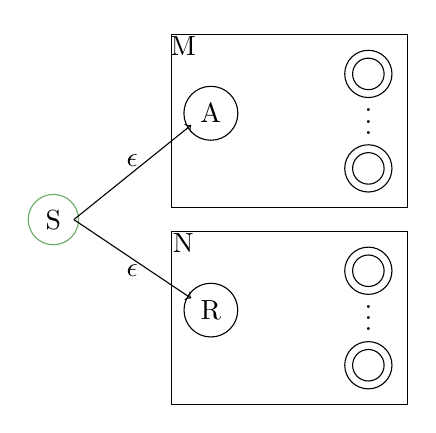
\begin{tikzpicture}
\draw (0,4.65) node[circle,draw,color=darkgreen] {\textcolor{black}{S}};
\draw (2,6) node[circle,draw] {A};
\draw (2,3.5) node[circle,draw] {R};
\draw[->] (0.26,4.65) -- (1.75,5.85);
\draw[->] (0.26,4.65) -- (1.75,3.65);
\draw (1,5.4) node {$\epsilon$};
\draw (1,4.0) node {$\epsilon$};
\draw (4,6.5) circle (0.2cm); % finals of M
\draw (4,6.5) circle (0.3cm);
\draw (4,6) node {\vdotss};
\draw (4,5.3) circle (0.2cm);
\draw (4,5.3) circle (0.3cm);
\draw (4,4) circle (0.2cm); % finals of N
\draw (4,4) circle (0.3cm);
\draw (4,3.5) node {\vdotss};
\draw (4,2.8) circle (0.2cm);
\draw (4,2.8) circle (0.3cm);
\draw (1.5,4.8) rectangle (4.5,7);
\draw (1.5,2.3) rectangle (4.5,4.5);
\draw (1.65,6.85) node {M};
\draw (1.65,4.35) node {N};
\end{tikzpicture}
\end{center}

\item<2-> Illustrate union-viz using closure-algorithms.rkt

\end{itemize}
\end{scriptsize}
\end{frame}

\begin{frame}[fragile]
\frametitle{FSA and Regular Expressions}
%\framesubtitle{HOMEWORK}
\begin{scriptsize}
\begin{itemize}
\item<1->
\begin{alltt}
;; ndfa ndfa \arrow ndfa
;; Purpose: Construct ndfa for the union of given ndfas
;; Assume: The intersection of states is empty
     (define (union-fsa M N)
\end{alltt}

\item<4->
\begin{alltt}
  (let* [(new-start (gen-state (append (sm-states M) (sm-states N))))
\end{alltt}

\item<5->
\begin{alltt}
         (new-sigma (remove-duplicates
                      (append (sm-sigma M) (sm-sigma N))))
\end{alltt}

\item<6->
\begin{alltt}
         (new-states (cons new-start
                           (append (sm-states M) (sm-states N))))
\end{alltt}

\item<7->
\begin{alltt}
         (new-finals (append (sm-finals M) (sm-finals N)))
\end{alltt}

\item<8->
\begin{alltt}
         (new-rules (append (list (list new-start EMP (sm-start M))
                                  (list new-start EMP (sm-start N)))
                            (sm-rules M)
                            (sm-rules N)))]
\end{alltt}

\item<9->
\begin{alltt}
   (make-ndfa new-states new-sigma new-start new-finals new-rules)))
\end{alltt}

\item<2->
\begin{alltt}
;; Tests for union-fsa
(define ab*Ua-aUb-b* (union-fsa ab* a-aUb-b*))
(define ab*Uaab* (union-fsa ab* aab*))
\end{alltt}

\item<3->
\begin{alltt}
(check-equal? (sm-apply ab*Ua-aUb-b* \elist) \quot{}reject)
(check-equal? (sm-apply ab*Ua-aUb-b* \quot{}(a a a a)) \quot{}reject)
(check-equal? (sm-apply ab*Ua-aUb-b* \quot{}(a b)) \quot{}accept)
(check-equal? (sm-apply ab*Ua-aUb-b* \quot{}(a a b b)) \quot{}accept)
(check-equal? (sm-testequiv? ab*Ua-aUb-b* (sm-union ab* ab*Ua-aUb-b*)) #t)
(check-equal? (sm-apply ab*Uaab* \quot{}(a a a)) \quot{}reject)
(check-equal? (sm-apply ab*Uaab* \quot{}(b a b a)) \quot{}reject)
(check-equal? (sm-apply ab*Uaab* \quot{}(a b b)) \quot{}accept)
(check-equal? (sm-apply ab*Uaab* \quot{}(a a b)) \quot{}accept)
(check-equal? (sm-apply ab*Uaab* \quot{}(a b b b b)) \quot{}accept)
(check-equal? (sm-testequiv? ab*Uaab* (sm-union ab* aab*)) #t)
\end{alltt}

\end{itemize}
\end{scriptsize}
\end{frame}

\begin{frame}[fragile]
\frametitle{FSA and Regular Expressions}
%\framesubtitle{HOMEWORK}
\begin{scriptsize}
\begin{lemma}
w$\in$L $\Leftrightarrow$ w$\in$L(U)
\end{lemma}

\begin{itemize}
\item<1-> Define three machines as follows:
\begin{alltt}
     M = (make-ndfa S \sig Z F \delt{})
     N = (make-ndfa S\quot{} \sig\quot{} Z\quot{} F\quot{} \delt{}\quot{})
     U = (union-fsa M N) = (make-ndfa S\quot{}\quot{} \sig\quot{}\quot{} Z\quot{}\quot{} F\quot{}\quot{} \delt{}\quot{}\quot{})
\end{alltt}

\item<1-> Let \texttt{L} = \texttt{L(M) $\cup$ L(N)}

\end{itemize}
\end{scriptsize}
\end{frame}

\begin{frame}[fragile]
\frametitle{FSA and Regular Expressions}
%\framesubtitle{HOMEWORK}
\begin{scriptsize}
\begin{lemma}
w$\in$L $\Leftrightarrow$ w$\in$L(U)
\end{lemma}

\begin{itemize}
\item<1-> ($\Rightarrow$) We need to show that w$\in$L $\Rightarrow$ w$\in$L(U)

\item<2-> Assume w$\in$L

\item<2-> This means that w$\in$L(M) or w$\in$L(N)

\item<2-> By construction, U nondeterministically correctly chooses to simulate M or to simulate N

\item<2-> Thus, w$\in$L(U).\\

\item<3-> ($\Leftarrow$) We need to show that w$\in$L(U) $\Rightarrow$ w$\in$L

\item<3-> Assume w$\in$L(U)

\item<3->This means that there is a computation that consumes w such that:
\begin{alltt}
     (w Z\quot{}\quot{}) \steps\(\sb{U}\) (() K), where K\(\in\)F\quot{}\quot{}
\end{alltt}

\item<4-> By U's construction, either M or N is simulated

\item<4-> U's final states are the final states of M and N

\item<4-> This means w$\in$L(M) or w$\in$L(N)

\item<4-> Thus, w$\in$L

\end{itemize}
\end{scriptsize}
\end{frame}

\begin{frame}[fragile]
\frametitle{FSA and Regular Expressions}
%\framesubtitle{HOMEWORK}
\begin{scriptsize}
\begin{lemma}
w$\notin$L $\Leftrightarrow$ w$\notin$L(U)
\end{lemma}

\begin{itemize}
\item<1-> ($\Rightarrow$) We need to show that w$\notin$L $\Rightarrow$ w$\notin$L(U)

\item<2-> Assume w$\notin$L

\item<2-> This means that w$\notin$L(M) and w$\notin$L(N)

\item<2-> By U's construction, F\quot{}\quot{} = F$\cup$F\quot{}

\item<2-> And all possible computations of U on w never reach a state in F\quot{}\quot{}

\item<2-> Thus, w$\notin$L(U)

\item<3-> ($\Leftarrow$) We need to show that w$\notin$L(U) $\Rightarrow$ w$\notin$L.\\

\item<4-> Assume w$\notin$L(U)

\item<4-> This means that all possible computations on w are described as follows:
\begin{alltt}
     (w Z\quot{}\quot{}) \steps\(\sb{U}\) (() K), where K\(\notin\)F\quot{}\quot{}
\end{alltt}

\item<4-> By U's construction, either M or N is simulated

\item<4-> F\quot{}\quot{} = F$\cup$F\quot{}

\item<4-> This means w$\notin$L(M) and w$\notin$L(N)

\item<4-> Thus, w$\notin$L

\end{itemize}
\end{scriptsize}
\end{frame}

\begin{frame}[fragile]
\frametitle{FSA and Regular Expressions}
%\framesubtitle{HOMEWORK}
\begin{scriptsize}
\begin{theorem}
The languages accepted by finite-state machines are closed under union.
\end{theorem}

\begin{itemize}
\item<1-> The theorem is established by the previous two lemmas

\end{itemize}
\end{scriptsize}
\end{frame}

\begin{frame}[fragile]
\frametitle{FSA and Regular Expressions}
%\framesubtitle{HOMEWORK}
\begin{scriptsize}
\begin{itemize}
\item<1-> HOMEWORK: 1, 3, 4

\end{itemize}
\end{scriptsize}
\end{frame}

\begin{frame}[fragile]
\frametitle{FSA and Regular Expressions}
%\framesubtitle{HOMEWORK}
\begin{scriptsize}
\begin{theorem}
The languages accepted by finite-state machines are closed concatenation.
\end{theorem}

\begin{itemize}
\item<1-> Let the following be the two machines that decide the languages to concatenate:
\begin{alltt}
     M = (make-ndfa S\(\sb{M}\) \sig\(\sb{\texttt{M}}\) A F\(\sb{M}\) \delt\(\sb{M}\))
     N = (make-ndfa S\(\sb{N}\) \sig\(\sb{\texttt{N}}\) R F\(\sb{N}\) \delt\(\sb{N}\))
\end{alltt}

\item<2-> We need to construct an \ndfa{} that decides \texttt{L = L(M) $\circ$ L(N)}

\item<3->
\begin{center}
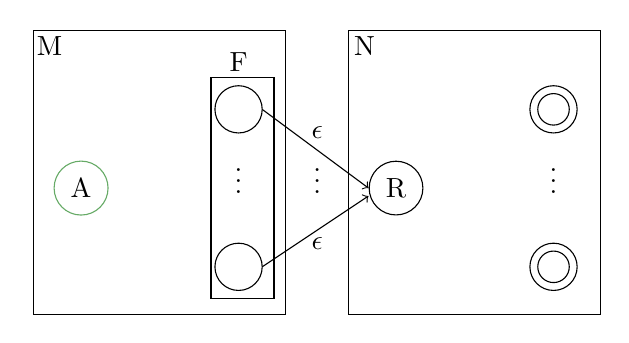
\begin{tikzpicture}
\draw (0,3) node[circle,draw,color=darkgreen] {\textcolor{black}{A}}; %M
%\draw (2,4) circle (0.2cm); % finals of M
\draw (2,4) circle (0.3cm);
\draw (2,3.2) node {\vdotss};
%\draw (2,2) circle (0.2cm);
\draw (2,2) circle (0.3cm);
\draw (-0.6,1.4) rectangle (2.6,5.0);
\draw (1.65,1.6) rectangle (2.45,4.4);
\draw (2,4.6) node {F};
\draw (-0.4,4.8) node {M};
\draw (4,3) node[circle,draw] {R}; %N
\draw (6,4) circle (0.2cm); % finals of N
\draw (6,4) circle (0.3cm);
\draw (6,3.2) node {\vdotss};
\draw (6,2) circle (0.2cm);
\draw (6,2) circle (0.3cm);
\draw (3.4,1.4) rectangle (6.6,5.0);
\draw (3.6,4.8) node {N};
\draw[->] (2.3,4) -- (3.65,3);
\draw[->] (2.3,2) -- (3.65,2.9);
\draw (3,3.7) node {$\epsilon$};
\draw (3,3.2) node {\vdotss};
\draw (3,2.3) node {$\epsilon$};
\end{tikzpicture}
\end{center}

\item<3-> Illustrate concat-viz using closure-algorithms.rkt

\end{itemize}
\end{scriptsize}
\end{frame}

\begin{frame}[fragile]
\frametitle{FSA and Regular Expressions}
%\framesubtitle{HOMEWORK}
\begin{scriptsize}
\begin{itemize}
\item<1->
\begin{alltt}
;; ndfa ndfa \arrow ndfa
;; Purpose: Construct ndfa for the concatenation of the languages of the
;;          given ndfas
;; Assume: The intersection of the states is empty
(define (concat-fsa M N)
\end{alltt}

\item<4->
\begin{alltt}
  (let* [(new-start (sm-start M))
\end{alltt}

\item<5->
\begin{alltt}
         (new-sigma (remove-duplicates (append (sm-sigma M) (sm-sigma N))))
\end{alltt}

\item<6->
\begin{alltt}
         (new-states (append (sm-states M) (sm-states N)))
\end{alltt}

\item<7->
\begin{alltt}
         (new-finals (sm-finals N))
\end{alltt}

\item<8->
\begin{alltt}
         (new-rules (append (sm-rules M)
                            (sm-rules N)
                            (map (\lamb (f) (list f EMP (sm-start N)))
                                 (sm-finals M))))]
\end{alltt}

\item<9->
\begin{alltt}
    (make-ndfa new-states new-sigma new-start new-finals new-rules)))
\end{alltt}

\item<2->
\begin{alltt}
;; Tests for concat-fsa
(define ab*-o-a-aUb-b* (concat-fsa ab* a-aUb-b*))
(define ab*-o-aab* (concat-fsa ab* aab*))
\end{alltt}

\item<3->
\begin{alltt}
(check-equal? (sm-apply ab*-o-a-aUb-b* \elist) \quot{}reject)
(check-equal? (sm-apply ab*-o-a-aUb-b* \quot{}(b b b)) \quot{}reject)
(check-equal? (sm-apply ab*-o-a-aUb-b* \quot{}(a a b a b)) \quot{}reject)
(check-equal? (sm-apply ab*-o-a-aUb-b* \quot{}(a b a a b)) \quot{}accept)
(check-equal? (sm-apply ab*-o-a-aUb-b* \quot{}(a b b b a a)) \quot{}accept)
(check-equal? (sm-testequiv? ab*-o-a-aUb-b* (sm-concat ab* a-aUb-b*)) #t)
(check-equal? (sm-apply ab*-o-aab* \elist) \quot{}reject)
(check-equal? (sm-apply ab*-o-aab* \quot{}(a b a)) \quot{}reject)
(check-equal? (sm-apply ab*-o-aab* \quot{}(a a b b a a)) \quot{}reject)
(check-equal? (sm-apply ab*-o-aab* \quot{}(a b b a a b b)) \quot{}accept)
(check-equal? (sm-apply ab*-o-aab* \quot{}(a a a)) \quot{}accept)
(check-equal? (sm-testequiv? ab*-o-aab* (sm-concat ab* aab*)) #t)
\end{alltt}

\end{itemize}
\end{scriptsize}
\end{frame}

\begin{frame}[fragile]
\frametitle{FSA and Regular Expressions}
%\framesubtitle{HOMEWORK}
\begin{scriptsize}
\begin{itemize}
\item<1-> Define three machines as follows:
\begin{alltt}
     M = (make-ndfa S \sig Z F \delt{})
     N = (make-ndfa S\quot{} \sig\quot{} Z\quot{} F\quot{} \delt{}\quot{})
     U = (concat-fsa M N) = (make-ndfa S\quot{}\quot{} \sig\quot{}\quot{} Z\quot{}\quot{} F\quot{}\quot{} \delt{}\quot{}\quot{})
\end{alltt}

\item<1-> Let \texttt{L} = \texttt{L(M) $\circ$ L(N)}

\item<1-> We proceed to prove that \texttt{L = L(U)}

\end{itemize}
\end{scriptsize}
\end{frame}

\begin{frame}[fragile]
\frametitle{FSA and Regular Expressions}
%\framesubtitle{HOMEWORK}
\begin{scriptsize}
\begin{lemma}
w$\in$L $\Leftrightarrow$ w$\in$L(U)
\end{lemma}

\begin{itemize}
\item<1-> ($\Rightarrow$) We need to show that w$\in$L $\Rightarrow$ w$\in$L(U)

\item<2-> Assume w$\in$L

\item<2-> This means w = xy, where x$\in$L(M) and y$\in$L(N)

\item<2-> By construction of U, the following is a valid computation:
\begin{alltt}
(xy S\quot{}\quot) \steps\(\sb{U)}\) (y R) \step{} (y Z\quot{}) \steps\(\sb{U}\) (() T), where R\(\in\)F and T\(\in\)F\quot{}
\end{alltt}

\item<2-> By construction of U, F\quot\quot = F\quot

\item<2-> Therefore, w$\in$L(U)

\item<3-> ($\Leftarrow$) We need to show that w$\in$L(U) $\Rightarrow$ w$\in$L

\item<4-> Assume w$\in$L(U)

\item<4-> By construction of U, this means that for w = xy the following computation is valid:
\begin{alltt}
(xy S\quot{}\quot) \steps\(\sb{U}\) (y R) \step{} (y Z\quot{}) \steps\(\sb{U}\) (() T), where R\(\in\)F and T\(\in\)F\quot{}
\end{alltt}

\item<4-> This implies that x$\in$L(M) and y$\in$L(N)

\item<4-> Thus, w$\in$L

\end{itemize}
\end{scriptsize}
\end{frame}

\begin{frame}[fragile]
\frametitle{FSA and Regular Expressions}
%\framesubtitle{HOMEWORK}
\begin{scriptsize}
\begin{lemma}
w$\notin$L $\Leftrightarrow$ w$\notin$L(U)
\end{lemma}

\begin{itemize}
\item<2-> ($\Rightarrow$) We need to show that w$\notin$L $\Rightarrow$ w$\notin$L(U)

\item<3-> Assume w$\notin$L

\item<3-> This means w $\neq$ xy, where x$\in$L(M) and y$\in$L(N)

\item<3-> By construction, all possible computations of U on w either do not reach a final state by consuming w or do not consume all of w

\item<3-> In both cases, w is rejected

\item<3-> Therefore, w$\notin$L(U).

\item<4-> ($\Leftarrow$) We need to show that w$\notin$L(U) $\Rightarrow$ w$\notin$L

\item<5-> Assume w$\notin$L(U)

\item<5-> By construction, this means that w is rejected because U consumes w and does not reach a final state or U is unable to consume w

\item<5-> This implies that w cannot be written as xy, where x$\in$L(M) and y$\in$L(N)

\item<5-> Thus, w$\notin$L

\end{itemize}
\end{scriptsize}
\end{frame}

\begin{frame}[fragile]
\frametitle{FSA and Regular Expressions}
%\framesubtitle{HOMEWORK}
\begin{scriptsize}
\begin{theorem}
The languages accepted by finite-state machines are closed concatenation.
\end{theorem}

\begin{itemize}
\item<1-> The proof follows from the two previous lemmas

\end{itemize}
\end{scriptsize}
\end{frame}

\begin{frame}[fragile]
\frametitle{FSA and Regular Expressions}
%\framesubtitle{HOMEWORK}
\begin{scriptsize}
\begin{itemize}
\item<1-> HOMEWORK: 5, 7, 8

\end{itemize}
\end{scriptsize}
\end{frame}

\begin{frame}[fragile]
\frametitle{FSA and Regular Expressions}
%\framesubtitle{HOMEWORK}
\begin{scriptsize}
\begin{theorem}
The languages accepted by finite-state machines are closed under Kleene star.
\end{theorem}

\begin{itemize}
\item<1-> Let the following be the machine that decides the language to be Kleene starred:
\begin{alltt}
     M = (make-ndfa S \sig A F \delt)
\end{alltt}

\item<1-> We need to construct an \ndfa{} that decides \texttt{L = L(M)$^{\texttt{*}}$}

\item<2->
\begin{center}
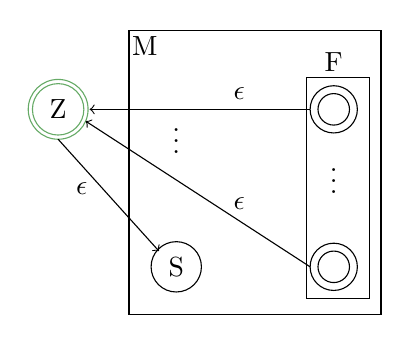
\begin{tikzpicture}
\draw (0,2) node[circle,draw] {S}; %M
\draw (2,4) circle (0.2cm); % finals of M
\draw (2,4) circle (0.3cm);
\draw (2,3.2) node {\vdotss};
\draw (2,2) circle (0.2cm);
\draw (2,2) circle (0.3cm);
\draw (-0.6,1.4) rectangle (2.6,5.0);
\draw (-0.4,4.8) node {M};
\draw (-1.5,4) node[circle,draw,color=darkgreen] {\textcolor{black}{Z}};
\draw[darkgreen] (-1.5,4) circle (0.38cm);
\draw[->] (-1.5,3.62) -- (-0.22,2.2);
\draw[->] (1.7,4) -- (-1.1,4);
\draw[->] (1.7,2) -- (-1.15,3.85);
\draw (0,3.7) node {\vdotss};
\draw (-1.20,3) node {$\epsilon$};
\draw (0.8,4.2) node {$\epsilon$};
\draw (0.8,2.8) node {$\epsilon$};
\draw (1.65,1.6) rectangle (2.45,4.4);
\draw (2,4.6) node {F};
\end{tikzpicture}
\end{center}

\item<2-> Illustrate kleenestar-viz using closure-algorithms.rkt

\end{itemize}
\end{scriptsize}
\end{frame}

\begin{frame}[fragile]
\frametitle{FSA and Regular Expressions}
%\framesubtitle{HOMEWORK}
\begin{tiny}
\begin{itemize}
\item<1->
\begin{alltt}
;; ndfa \arrow ndfa
;; Purpose: Construct ndfa for the Kleene star of given ndfa
(define (kstar-fsa M)
\end{alltt}

\item<3->
\begin{alltt}
  (let* [(new-start (generate-symbol \quot{}K (sm-states M)))
         (new-sigma (sm-sigma M))
\end{alltt}

\item<4->
\begin{alltt}
         (new-states (cons new-start (sm-states M)))
         (new-finals (cons new-start (sm-finals M)))
\end{alltt}

\item<5->
\begin{alltt}
         (new-rules (cons (list new-start EMP (sm-start M))
                          (append (sm-rules M)
                                  (map (\lamb (f) (list f EMP new-start))
                                       (sm-finals M)))))]
\end{alltt}

\item<6->
\begin{alltt}
    (make-ndfa new-states new-sigma new-start new-finals new-rules)))
\end{alltt}

\item<2->
\begin{alltt}
;; Tests for kstar-fsa
(define a-aUb-b*-* (kstar-fsa a-aUb-b*))
(define ab*-* (kstar-fsa ab*))

(check-equal? (sm-apply a-aUb-b*-* \quot{}(b b b)) \quot{}reject)
(check-equal? (sm-apply a-aUb-b*-* \quot{}(a b a b a a a a)) \quot{}reject)
(check-equal? (sm-apply a-aUb-b*-* \elist) \quot{}accept)
(check-equal? (sm-apply a-aUb-b*-* \quot{}(a a a a b b b b)) \quot{}accept)
(check-equal? (sm-apply a-aUb-b*-* \quot{}(a a b a a b b a a)) \quot{}accept)
(check-equal? (sm-testequiv? a-aUb-b*-* (sm-kleenestar a-aUb-b*)) #t)

(check-equal? (sm-apply ab*-* \quot{}(b)) \quot{}reject)
(check-equal? (sm-apply ab*-* \quot{}(b b b)) \quot{}reject)
(check-equal? (sm-apply ab*-* \elist) \quot{}accept)
(check-equal? (sm-apply ab*-* \quot{}(a a a a)) \quot{}accept)
(check-equal? (sm-apply ab*-* \quot{}(a b a b b a b b b)) \quot{}accept)
(check-equal? (sm-testequiv? ab*-* (sm-kleenestar ab*)) #t)
\end{alltt}

\end{itemize}
\end{tiny}
\end{frame}

\begin{frame}[fragile]
\frametitle{FSA and Regular Expressions}
%\framesubtitle{HOMEWORK}
\begin{scriptsize}
\begin{itemize}
\item<1-> Define two machines as follows:
\begin{alltt}
     M = (make-ndfa S \sig Z F \delt{})
     U = (kstar-fsa M) = (make-ndfa S\quot{} \sig\quot{} Z\quot{} F\quot{} \delt{}\quot{})
\end{alltt}

\item<2-> Let \texttt{L} = \texttt{L(M)$^{\texttt{*}}$}

\item<2-> We proceed to prove that \texttt{L = L(U)}

\end{itemize}
\end{scriptsize}
\end{frame}

\begin{frame}[fragile]
\frametitle{FSA and Regular Expressions}
%\framesubtitle{HOMEWORK}
\begin{scriptsize}
\begin{lemma}
w$\in$L $\Leftrightarrow$ w$\in$L(U)
\end{lemma}

\begin{itemize}
\item<1-> ($\Rightarrow$) We need to show that w$\in$L $\Rightarrow$ w$\in$L(U)

\item<2-> Assume w$\in$L. This means that w = w$_1$w$_2$\dotss{}w$_n$,
where w$_i$$\in$L(M)

\item<2-> By construction of U, the following is a computation on w:
\begin{alltt}
((w\(\sb{1}\)w\(\sb{2}\)\dotss{}w\(\sb{n}\) S\quot{}) \steps$_U$ ((w\(\sb{2}\)\dotss{}w\(\sb{n}\)) Y\(\sb{1}\)) \steps\(\sb{U}\) ((\dotss{}w\(\sb{n}\)) Y\(\sb{2}\)) \steps\(\sb{U}\) (() Y\(\sb{n}\)),
where Y\(\sb{i}\)\(\in\)F\quot{}
\end{alltt}

\item<2-> Therefore, w$\in$L(U)

\item<3-> ($\Leftarrow$) We need to show that w$\in$L(U) $\Rightarrow$ w$\in$L\\

\item<4-> Assume w$\in$L(U)

\item<4-> This means that w = w$_1$w$_2$\dotss{}w$_n$ such that:
\begin{alltt}
\noindent ((w\(\sb{1}\)\dotss{}w\(\sb{n}\)) S\quot{}) \steps\(\sb{U}\) ((w\(\sb{2}\)\dotss{}w\(\sb{n}\)) Y\(\sb{1}\)) \steps\(\sb{U}\) ((w\(\sb{3}\)\dotss{}w\(\sb{n}\)) Y\(\sb{2}\))\dotss{}((w\(\sb{n}\)) Y\(\sb{n-1}\))
\steps\(\sb{U}\) (() Y\(\sb{n}\)), where Y\(\sb{i}\)\(\in\)F\quot{}
\end{alltt}

\item<4-> By construction of U, F\quot{} contains S\quot{} and F

\item<4-> This means that w is the concatenation of zero or more words in L(M)

\item<4-> Thus, w$\in$L

\end{itemize}
\end{scriptsize}
\end{frame}

\begin{frame}[fragile]
\frametitle{FSA and Regular Expressions}
%\framesubtitle{HOMEWORK}
\begin{scriptsize}
\begin{lemma}
w$\notin$L $\Leftrightarrow$ w$\notin$L(U)
\end{lemma}

\begin{itemize}
\item<1-> ($\Rightarrow$)

\item<1-> We need to show that w$\notin$L $\Rightarrow$ w$\notin$L(U)

\item<2-> Assume w$\notin$L

\item<2-> This means that w $\neq$ w$_1$w$_2$\dotss{}w$_n$, where w$_i$$\in$L(M)

\item<2-> By construction of U, the processing of w can occur in two ways

\item<2-> The first, w is consumed and U does not end in a final state

\item<2-> The second, w cannot be completely consumed

\item<2-> In both cases, w is rejected

\item<2-> Thus, w$\notin$L(U).

\item<3-> ($\Leftarrow$) We need to show that w$\notin$L(U) $\Rightarrow$ w$\notin$L

\item<4-> Assume w$\notin$L(U)

\item<4-> This means that w $\neq$ w$_1$w$_2$\dotss{}w$_n$ such that:
\begin{alltt}
\noindent ((w\(\sb{1}\)\dotss{}w\(\sb{n}\)) S\quot{}) \steps\(\sb{U}\) ((w\(\sb{2}\)\dotss{}w\(\sb{n}\)) Y\(\sb{1}\)) \steps\(\sb{U}\) ((w\(\sb{3}\)\dotss{}w$_\(\sb{n}\)) Y\(\sb{2}\))\dotss{}((w\(\sb{n}\)) Y\(\sb{n-1}\))
\steps\(\sb{U}\) (() Y\(\sb{n}\)), where Y\(\sb{n}\)\(\in\)F\quot{}
\end{alltt}

\item<4-> By construction of U, F\quot{} contains S\quot{} and F

\item<4-> This means that w is not the concatenation of zero or more words in L(M)

\item<4-> Thus, w$\notin$L

\end{itemize}
\end{scriptsize}
\end{frame}

\begin{frame}[fragile]
\frametitle{FSA and Regular Expressions}
%\framesubtitle{HOMEWORK}
\begin{scriptsize}
\begin{theorem}
The languages accepted by finite-state machines are closed under Kleene star.
\end{theorem}

\begin{itemize}
\item<1-> The proof follows from the previous two lemmas

\end{itemize}
\end{scriptsize}
\end{frame}

\begin{frame}[fragile]
\frametitle{FSA and Regular Expressions}
%\framesubtitle{HOMEWORK}
\begin{scriptsize}
\begin{itemize}
\item<1-> HOMEWORK: 10, 11

\item<1-> QUIZ: 9

\end{itemize}
\end{scriptsize}
\end{frame}

\begin{frame}[fragile]
\frametitle{FSA and Regular Expressions}
%\framesubtitle{HOMEWORK}
\begin{scriptsize}
\begin{theorem}
The languages accepted by finite-state machines are closed under complement.
\end{theorem}

\begin{itemize}
\item<1-> Let \texttt{M} be a \dfa. The complement of \texttt{L(M)} is defined as follows:
\begin{alltt}
     \={L(M)} = \{w | w\(\notin\)L(M)\}
\end{alltt}

\item<2-> The complement of \texttt{L(M)} is the language that contains all words not in \texttt{L(M)}

\item<3-> Given that \texttt{M} is a \dfa{}, this suggests inverting the roles of \texttt{M}'s states

\item<4->
\begin{center}
\includegraphics[scale=0.5]{a-star-graph.png}
\end{center}

\item<4-> Reversing the roles of the states yields:
\begin{center}
\includegraphics[scale=0.5]{not-a-star-graph.png}
\end{center}

\item<4-> Illustrate complement-viz using closure-algorithms.rkt

\end{itemize}
\end{scriptsize}
\end{frame}

\begin{frame}[fragile]
\frametitle{FSA and Regular Expressions}
%\framesubtitle{HOMEWORK}
\begin{scriptsize}
\begin{itemize}
\item<1->
\begin{alltt}
;; dfa \arrow dfa
;; Purpose: Construct a dfa for the complement of given dfa's language
(define (complement-fsa M)
\end{alltt}

\item<3->
\begin{alltt}
  (let* [(new-finals (filter (\lamb (s) (not (member s (sm-finals M))))
                             (sm-states M)))]
\end{alltt}

\item<4->
\begin{alltt}
    (make-dfa (sm-states M)
              (sm-sigma M)
              (sm-start M)
              new-finals
              (sm-rules M)
              \quot{}no-dead)))
\end{alltt}

\item<2->
\begin{alltt}
;; Tests for complement-fsa
(define not-a* (complement-fsa a*))
(define not-EVEN-A-ODD-B (complement-fsa EVEN-A-ODD-B))

(check-equal? (sm-apply not-a* \elist) \quot{}reject)
(check-equal? (sm-apply not-a* \quot{}(a a a)) \quot{}reject)
(check-equal? (sm-apply not-a* \quot{}(a a b)) \quot{}accept)
(check-equal? (sm-apply not-a* \quot{}(b b a a b)) \quot{}accept)
(check-equal? (sm-testequiv? not-a* (sm-complement a*)) #t)

(check-equal? (sm-apply not-EVEN-A-ODD-B \quot{}(b)) \quot{}reject)
(check-equal? (sm-apply not-EVEN-A-ODD-B \quot{}(a a b)) \quot{}reject)
(check-equal? (sm-apply not-EVEN-A-ODD-B \quot{}(b b a b a)) \quot{}reject)
(check-equal? (sm-apply not-EVEN-A-ODD-B \elist) \quot{}accept)
(check-equal? (sm-apply not-EVEN-A-ODD-B \quot{}(b b a a)) \quot{}accept)
(check-equal? (sm-apply not-EVEN-A-ODD-B \quot{}(a a b b a b)) \quot{}accept)
(check-equal? (sm-testequiv? not-EVEN-A-ODD-B
                             (sm-complement EVEN-A-ODD-B))
              #t)
\end{alltt}

\end{itemize}
\end{scriptsize}
\end{frame}

\begin{frame}[fragile]
\frametitle{FSA and Regular Expressions}
%\framesubtitle{HOMEWORK}
\begin{scriptsize}
\begin{itemize}
\item<1-> Define two machines as follows:
\begin{alltt}
     M = (make-dfa S \sig Z F \delt{})
     U = (complement-fsa M) = (make-ndfa S \sig Z F\quot{} \delt{})
\end{alltt}

\item<1-> Let \texttt{L} = \texttt{\={L(M)}}

\item<1-> We proceed to prove that \texttt{L = L(U)}

\end{itemize}
\end{scriptsize}
\end{frame}

\begin{frame}[fragile]
\frametitle{FSA and Regular Expressions}
%\framesubtitle{HOMEWORK}
\begin{scriptsize}
\begin{lemma}
w$\in$L $\Leftrightarrow$ w$\notin$L(U)
\end{lemma}

\begin{itemize}
\item<1-> ($\Rightarrow$)

\item<1-> We need to show that w$\in$L $\Rightarrow$ w$\notin$L(U)

\item<2-> Assume w$\in$L

\item<2-> Given that M is a \dfa, the following is the computation performed on w:
\begin{alltt}
((w) S) \steps\(\sb{M}\) (() Q), where Q\(\in\)F
\end{alltt}

\item<2-> By construction of U, Q$\notin$F\quot{} and M performs the same computation moving from S to Q by consuming w

\item<2-> Therefore, w$\notin$L(U)

\item<3-> ($\Leftarrow$) We need to show that w$\notin$L(U) $\Rightarrow$ w$\in$L\\

\item<4-> Assume w$\notin$L(U)

\item<4-> This means that U performs the following computation on w:
\begin{alltt}
((w) S) \steps\(\sb{U}\) (() Q), where Q\(\notin\)F\quot{}
\end{alltt}

\item<4-> By construction of U, Q$\in$F and M performs the same computation moving from S to Q by consuming w

\item<4-> Thus, w$\in$L

\end{itemize}
\end{scriptsize}
\end{frame}

\begin{frame}[fragile]
\frametitle{FSA and Regular Expressions}
%\framesubtitle{HOMEWORK}
\begin{scriptsize}
\begin{lemma}
w$\notin$L $\Leftrightarrow$ w$\in$L(U)
\end{lemma}

\begin{itemize}
\item<1-> ($\Rightarrow$) We need to show that w$\notin$L $\Rightarrow$ w$\in$L(U)

\item<2-> Assume w$\notin$L

\item<2-> Given that M is a \dfa, the following is the computation it performs on w:
\begin{alltt}
((w) S) \steps\(\sb{M}\) (() Q), where Q\(\notin\)F
\end{alltt}

\item<2-> By construction of U, Q$\in$F\quot{} and U performs the same computation moving from S to Q by consuming w

\item<2-> Therefore, w$\in$L(U).\\

\item<3-> ($\Leftarrow$) We need to show that w$\in$L(U) $\Rightarrow$ w$\notin$L

\item<4-> Assume w$\in$L(U)

\item<4-> This means that U performs the following computation on w:
\begin{alltt}
((w) S) \steps\(\sb{U}\) (() Q), where Q\(\in\)F\quot{}
\end{alltt}

\item<4-> By construction of U, Q$\notin$F and M performs the same computation moving from S to Q by consuming w

\item<4-> Thus, w$\notin$L

\end{itemize}
\end{scriptsize}
\end{frame}

\begin{frame}[fragile]
\frametitle{FSA and Regular Expressions}
%\framesubtitle{HOMEWORK}
\begin{scriptsize}
\begin{theorem}
The languages accepted by finite-state machines are closed under complement.
\end{theorem}

\begin{itemize}
\item<1-> The proof follows from the previous two lemmas

\end{itemize}
\end{scriptsize}
\end{frame}

\begin{frame}[fragile]
\frametitle{FSA and Regular Expressions}
%\framesubtitle{HOMEWORK}
\begin{scriptsize}
\begin{itemize}
\item<1-> HOMEWORK: 12, 14

\end{itemize}
\end{scriptsize}
\end{frame}

\begin{frame}[fragile]
\frametitle{FSA and Regular Expressions}
%\framesubtitle{HOMEWORK}
\begin{scriptsize}
\begin{theorem}
The languages decided by finite-state automatons are closed under intersection.
\end{theorem}
\begin{itemize}
\item<1->
\begin{alltt}
     M = (make-ndfa S\(\sb{M}\) \sig\(\sb{M}\) A F\(\sb{M}\) \delt\(\sb{M}\))
     N = (make-ndfa S\(\sb{N}\) \sig\(\sb{N}\) R F\(\sb{N}\) \delt\(\sb{N}\))
\end{alltt}

\item<1-> We need to construct an \ndfa{} that accepts and only accepts the words in \texttt{L(M)$\cap$L(N)}

\item<2-> Consider the following facts from set theory:
\begin{alltt}
     \sig\(\sp{*}\) - B = \{w | w\(\in\)\sig\(\sp{*}\) \(\wedge\) w\(\notin\)B\}
     \sig\(\sp{*}\) - A = \{w | w\(\in\)\sig\(\sp{*}\) \(\wedge\) w\(\notin\)A\}
\end{alltt}

\item<2-> All possible words in \sig$^*$ that are not in \texttt{B} and all possible words in \sig$^*$ that are not in \texttt{A}

\item<3-> Consider the union of these two sets:
\begin{alltt}
     \{\sig\(\sp{*}\) - B\} \(\cup\) \{\sig\(\sp{*}\) - A\} = \{w | w\(\notin\)A \(\wedge\) w\(\notin\)B\}
\end{alltt}

\item<3-> What words are not contained in this union?

\item<4-> It is exactly the elements that are in both \texttt{A} and \texttt{B}

\item<5-> We may define the language for the machine we wish to implement as follows:
\begin{alltt}
     L(M)\(\cap\)L(N) = \sig\(\sp{*}\) - \{\{\sig\(\sp{*}\) - L(M)\} \(\cup\) \{\sig\(\sp{*}\) - L(N)\}\}
                = \sig\(\sp{*}\) - \{\={L(M)} \(\cup\) \={L(N)}\}
\end{alltt}

\item<5-> Illustrate intersection-viz using closure-algorithms.rkt

\end{itemize}
\end{scriptsize}
\end{frame}

\begin{frame}[fragile]
\frametitle{FSA and Regular Expressions}
%\framesubtitle{HOMEWORK}
\begin{scriptsize}
\begin{itemize}
\item<1->
\begin{alltt}
;; ndfa ndfa \arrow ndfa
;; Purpose: Construct an ndfa for the intersection of the languages of the
;;          given ndfas
(define (intersect-fsa M N)
\end{alltt}

\item<3->
\begin{alltt}
  (let* [(notM (sm-rename-states
                 (list DEAD)
                 (sm-complement (ndfa->dfa M))))
         (notN (sm-rename-states
                 (list DEAD)
                 (sm-complement (ndfa->dfa N))))]
\end{alltt}

\item<4->
\begin{alltt}
    (complement-fsa (ndfa->dfa (sm-union notM notN)))))
\end{alltt}

\item<2->
\begin{alltt}
;; Tests for intersect-fsa
(define ab*-intersect-a-aUb-b* (intersect-fsa ab* a-aUb-b*))
(define a-aUb-b*-intersect-EVEN-A-ODD-B (intersect-fsa  a-aUb-b*
                                                        EVEN-A-ODD-B))

(check-equal? (sm-apply ab*-intersect-a-aUb-b* \elist) \quot{}reject)
(check-equal? (sm-apply ab*-intersect-a-aUb-b* \quot{}(a b b a)) \quot{}reject)
(check-equal? (sm-apply ab*-intersect-a-aUb-b* \quot{}(a b)) \quot{}reject)
(check-equal? (sm-testequiv? ab*-intersect-a-aUb-b*
                             (sm-intersection ab* a-aUb-b*))
              #t)

(check-equal? (sm-apply a-aUb-b*-intersect-EVEN-A-ODD-B \elist) \quot{}reject)
(check-equal? (sm-apply a-aUb-b*-intersect-EVEN-A-ODD-B \quot{}(b b)) \quot{}reject)
(check-equal? (sm-apply a-aUb-b*-intersect-EVEN-A-ODD-B \quot{}(a a b b)) \quot{}reject)
(check-equal? (sm-apply a-aUb-b*-intersect-EVEN-A-ODD-B \quot{}(a a b)) \quot{}accept)
(check-equal? (sm-apply a-aUb-b*-intersect-EVEN-A-ODD-B \quot{}(a a b b b)) \quot{}accept)
(check-equal? (sm-testequiv? a-aUb-b*-intersect-EVEN-A-ODD-B
                             (sm-intersection a-aUb-b* EVEN-A-ODD-B))
              #t)
\end{alltt}

\end{itemize}
\end{scriptsize}
\end{frame}

\begin{frame}[fragile]
\frametitle{FSA and Regular Expressions}
%\framesubtitle{HOMEWORK}
\begin{scriptsize}
\begin{itemize}
\item<1-> Define three machines as follows:
\begin{alltt}
     M = (make-ndfa S \sig Z F \delt{})
     N = (make-ndfa S\quot{} \sig\quot{} Z\quot{} F\quot{} \delt{}\quot{})
     U = (intersect-fsa M N) = (make-ndfa S\quot{}\quot{} \sig\quot{}\quot{} Z\quot{}\quot{} F\quot{}\quot{} \delt{}\quot{}\quot{})
\end{alltt}

\item<1-> Let \texttt{L} = \texttt{L(M) $\cap$ L(N)}

\item<1-> We proceed to prove that \texttt{L = L(U)}

\end{itemize}
\end{scriptsize}
\end{frame}

\begin{frame}[fragile]
\frametitle{FSA and Regular Expressions}
%\framesubtitle{HOMEWORK}
\begin{scriptsize}
\begin{lemma}
w$\in$L $\Leftrightarrow$ w$\in$L(U)
\end{lemma}

\begin{itemize}
\item<1-> ($\Rightarrow$) We need to show that w$\in$L $\Rightarrow$ w$\in$L(U)

\item<2-> Assume w$\in$L

\item<2-> This means that w$\in$L(M) and w$\in$L(N)

\item<2-> Therefore, w$\in$(\sig\(\sp{*}\) - \{\={L(M)} \(\cup\) \={L(N)}\})

\item<2-> By construction of U, w$\in$L(U)

\item<3-> ($\Leftarrow$) We need to show that w$\in$L(U) $\Rightarrow$ w$\in$L

\item<4-> Assume w$\in$L(U)

\item<4-> By U's construction, w$\in$(\sig\(\sp{*}\) - \{\={L(M)} \(\cup\) \={L(N)}\})

\item<4-> Therefore, w$\in$L(M) and w$\in$L(N)

\item<4-> Thus, w$\in$L

\end{itemize}
\end{scriptsize}
\end{frame}

\begin{frame}[fragile]
\frametitle{FSA and Regular Expressions}
%\framesubtitle{HOMEWORK}
\begin{scriptsize}
\begin{lemma}
w$\notin$L $\Leftrightarrow$ w$\notin$L(U)
\end{lemma}

\begin{itemize}
\item<1-> ($\Rightarrow$) We need to show that w$\notin$L $\Rightarrow$ w$\notin$L(U)

\item<2-> Assume w$\notin$L

\item<2-> This means that w$\notin$L(M) or w$\notin$L(N)

\item<2-> Therefore, w$\notin$(\sig\(\sp{*}\) - \{\={L(M)} \(\cup\) \={L(N)}\})

\item<2-> By construction of U, w$\notin$L(U)

\item<3-> ($\Leftarrow$) We need to show that w$\notin$L(U) $\Rightarrow$ w$\notin$L

\item<4-> Assume w$\notin$L(U)

\item<4-> By U's construction, w$\notin$(\sig\(\sp{*}\) - \{\={L(M)} \(\cup\) \={L(N)}\})

\item<4-> Therefore, w$\notin$L(M) or w$\notin$L(N)

\item<4-> Thus, w$\notin$L

\end{itemize}
\end{scriptsize}
\end{frame}

\begin{frame}[fragile]
\frametitle{FSA and Regular Expressions}
%\framesubtitle{HOMEWORK}
\begin{scriptsize}
\begin{theorem}
The languages decided by finite-state automatons are closed under intersection.
\end{theorem}

\begin{itemize}
\item<1-> The proof follows from the previous two lemmas

\end{itemize}
\end{scriptsize}
\end{frame}

\begin{frame}[fragile]
\frametitle{FSA and Regular Expressions}
%\framesubtitle{HOMEWORK}
\begin{scriptsize}
\begin{itemize}
\item<1-> HOMEWORK: 15

\item<1-> Quiz: 16 (due in 1 week)

\end{itemize}
\end{scriptsize}
\end{frame}

\begin{frame}[fragile]
\frametitle{FSA and Regular Expressions}
%\framesubtitle{HOMEWORK}
\begin{scriptsize}
\begin{itemize}
\item<1-> Is there a finite-state machine for the language of any regular expression?

\item<2-> Is there is a regular expression for any language decided by a finite-state machine?

\item<3-> Our goal: establish the equivalence of finite-state machines and regular expressions

\end{itemize}
\end{scriptsize}
\end{frame}

\begin{frame}[fragile]
\frametitle{FSA and Regular Expressions}
%\framesubtitle{HOMEWORK}
\begin{scriptsize}
\begin{itemize}
\item<1-> We start by proving that there is a finite-state machine that decides the language of a regular expression

\item<2-> Think about the structure of a regular expression

\item<2-> A regular expression may the thought of as a tree

\item<2-> The empty regular expression and the singleton regular expressions are leaves

\item<2-> The concatenation, union, and Kleene star regular expressions are interior nodes

\item<3-> \texttt{ab $\cup$ bb$^{\texttt{*}}$}
\begin{center}
\scalebox{0.6}{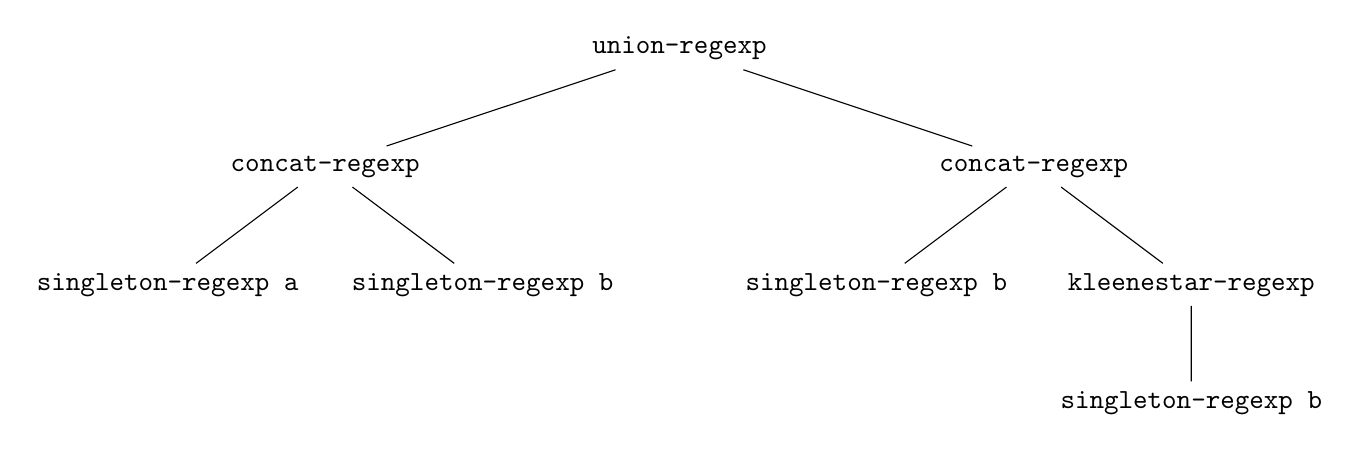
\begin{tikzpicture}[level distance=1.5cm,level 1/.style={sibling distance=9cm},level 2/.style={sibling distance=4cm},level 3/.style={sibling distance=3cm}]
    \node {\texttt{union-regexp}}
      child {node {\texttt{concat-regexp}}
        child {node {\texttt{singleton-regexp a}}}
        child {node {\texttt{singleton-regexp b}}}}
      child {node {\texttt{concat-regexp}}
        child {node {\texttt{singleton-regexp b}}}
        child {node {\texttt{kleenestar-regexp}}
          child {node {\texttt{singleton-regexp b}}}}};
    \end{tikzpicture}}
\end{center}

\item<3-> A regular expression may be processed using structural recursion

\end{itemize}
\end{scriptsize}
\end{frame}

\begin{frame}[fragile]
\frametitle{FSA and Regular Expressions}
%\framesubtitle{HOMEWORK}
\begin{scriptsize}
\begin{itemize}
\item<1-> To build an \ndfa{}, a regular expression, \texttt{e}, and the language's alphabet, \sig, are needed

\item<2-> The subtype of the given regular expression is determined and the appropriate \ndfa{} is constructed

\item<3-> If the subtype  is an empty regular expression then an \ndfa{} that only accepts empty is returned.

\item<4-> If the subtype is a singleton regular expression for \texttt{x$\in$\sig} then an \ndfa{} that only accepts \texttt{x} is returned

\item<5-> If the subtype is a union regular expression then closure under union is used

\item<6-> If the subtype is a concatenation regular expression then closure inder concatenation is used

\item<7-> If the subtype is a Kleene star regular expression then closure under Kleene star is used
    
\item<7-> Illustrate using regexp2ndfa.rkt

\end{itemize}
\end{scriptsize}
\end{frame}

\begin{frame}[fragile]
\frametitle{FSA and Regular Expressions}
%\framesubtitle{HOMEWORK}
\begin{scriptsize}
\begin{itemize}
\item<1->
\begin{alltt}
;; regexp alphabet \arrow ndfa   Purpose: Build ndfa for given regexp
(define (regexp->ndfa e sigma)

\end{alltt}

\end{itemize}
\end{scriptsize}
\end{frame}

\begin{frame}[fragile]
\frametitle{FSA and Regular Expressions}
%\framesubtitle{HOMEWORK}
\begin{tiny}
\begin{itemize}
\item<1->
\begin{alltt}
;; Tests for reg-exp->ndfa
(define e (empty-regexp))
(define a (singleton-regexp "a"))
(define b (singleton-regexp "b"))
(define ab (concat-regexp a b))
(define aa (concat-regexp a a))
(define abUe (union-regexp ab e))
(define abUaa (union-regexp ab aa))
(define aa-* (kleenestar-regexp aa))
(define abUaa-* (kleenestar-regexp abUaa))
\end{alltt}

\item<2->
\begin{alltt}
(define Me (regexp->ndfa e \quot{}(a b)))
(define Ma (regexp->ndfa a \quot{}(a b)))
(define Mb (regexp->ndfa b \quot{}(a b)))
(define Mab (regexp->ndfa ab \quot{}(a b)))
(define Maa (regexp->ndfa aa \quot{}(a b)))
(define MabUMe (regexp->ndfa abUe \quot{}(a b)))
(define MabUaa (regexp->ndfa abUaa \quot{}(a b)))
(define Maa-* (regexp->ndfa aa-* \quot{}(a b)))
(define MabUaa-* (regexp->ndfa abUaa-* \quot{}(a b)))
\end{alltt}

\item<3->
\begin{alltt}
(check-equal? (sm-apply Me \quot{}(a)) \quot{}reject)
(check-equal? (sm-apply Me \elist) \quot{}accept)
(check-equal? (sm-apply Ma \quot{}(b)) \quot{}reject)
(check-equal? (sm-apply Ma \quot{}(a)) \quot{}accept)
(check-equal? (sm-apply Mab \elist) \quot{}reject)
(check-equal? (sm-apply Mab \quot{}(a b)) \quot{}accept)
(check-equal? (sm-apply Maa \quot{}(b a a)) \quot{}reject)
(check-equal? (sm-apply Maa \quot{}(a a)) \quot{}accept)
(check-equal? (sm-apply MabUMe \quot{}(a b a a)) \quot{}reject)
(check-equal? (sm-apply MabUMe \quot{}(b b)) \quot{}reject)
(check-equal? (sm-apply MabUMe \elist) \quot{}accept)
(check-equal? (sm-apply MabUMe \quot{}(a b)) \quot{}accept)
(check-equal? (sm-apply MabUaa \quot{}(a b b b)) \quot{}reject)
(check-equal? (sm-apply MabUaa \quot{}(b a b)) \quot{}reject)
(check-equal? (sm-apply MabUaa \quot{}(a a)) \quot{}accept)
(check-equal? (sm-apply MabUaa \quot{}(a b)) \quot{}accept)
(check-equal? (sm-apply Maa-* \quot{}(a b)) \quot{}reject)
(check-equal? (sm-apply Maa-* \quot{}(a a a)) \quot{}reject)
(check-equal? (sm-apply Maa-* \quot{}(a a)) \quot{}accept)
(check-equal? (sm-apply Maa-* \quot{}(a a a a a a)) \quot{}accept)
(check-equal? (sm-apply MabUaa-* \quot{}(a b a)) \quot{}reject)
(check-equal? (sm-apply MabUaa-* \quot{}(b b b b)) \quot{}reject)
(check-equal? (sm-apply MabUaa-* \elist) \quot{}accept)
(check-equal? (sm-apply MabUaa-* \quot{}(a a a a a b)) \quot{}accept)
\end{alltt}

\end{itemize}
\end{tiny}
\end{frame}

\begin{frame}[fragile]
\frametitle{FSA and Regular Expressions}
%\framesubtitle{HOMEWORK}
\begin{tiny}
\begin{itemize}
\item<1->
\begin{alltt}
;; regexp alphabet \arrow ndfa  Purpose: Build ndfa for given regexp
(define (regexp->ndfa e sigma)
  (let* [(st-pairs (foldl (\lamb{} (s acc) \textcolor{red}{from-to state pairs}
                            (let* [(used-st-names (flatten acc))
                                   (from-state (gen-state used-st-names))
                                   (to-state (gen-state (cons from-state used-st-names)))]
                              (cons (list from-state to-state) acc)))
                          \elist
                          (cons EMP sigma)))
         (simple-tbl (map (\lamb{} (p a) (list a
             \textcolor{red}{singleton machines}          (make-ndfa p
                                                    sigma
                                                    (first p)
                                                    (list (second p))
                                                    (list (list (first p) a (second p))))))
                          st-pairs
                          (cons EMP sigma)))]
\end{alltt}

\item<2->
\begin{alltt}
    (cond [(empty-regexp? e) (second (assoc EMP simple-tbl))]
\end{alltt}

\item<3->
\begin{alltt}
          [(singleton-regexp? e)
           (second (assoc (string->symbol (singleton-regexp-a e)) simple-tbl))]
\end{alltt}

\item<4->
\begin{alltt}
          [(concat-regexp? e)
           (let* [(M (regexp->ndfa (concat-regexp-r1 e) sigma))
                  (N (sm-rename-states (sm-states M)
                                       (regexp->ndfa (concat-regexp-r2 e) sigma)))]
           (concat-fsa M N))]
\end{alltt}

\item<5->
\begin{alltt}
          [(union-regexp? e)
           (let* [(M (regexp->ndfa (union-regexp-r1 e) sigma))
                  (N (sm-rename-states (sm-states M)
                                       (regexp->ndfa (union-regexp-r2 e) sigma)))]
           (union-fsa M N))]
\end{alltt}

\item<6->
\begin{alltt}
          [else (kstar-fsa (regexp->ndfa (kleenestar-regexp-r1 e)
                           sigma))])))
\end{alltt}

\end{itemize}
\end{tiny}
\end{frame}

\begin{frame}[fragile]
\frametitle{FSA and Regular Expressions}
%\framesubtitle{HOMEWORK}
\begin{scriptsize}
\begin{itemize}
\item<1-> we shall prove that \texttt{regexp->ndfa} is correct

\item<1-> Given that \texttt{regexp->ndfa} uses structural recursion on a binary tree, the proof is by induction on the height of the binary tree

\end{itemize}
\end{scriptsize}
\end{frame}

\begin{frame}[fragile]
\frametitle{FSA and Regular Expressions}
%\framesubtitle{HOMEWORK}
\begin{scriptsize}
\begin{theorem}
L is a regular language $\Rightarrow$ L is decided by a finite-state machine.
\end{theorem}

\begin{itemize}
\item<1-> Assume L is regular

\item<2-> This means that there is a regular expression, R, that defines L

\item<2-> Let \sig{} be the alphabet for the language of R

\item<2-> We prove by induction on the height of R that \texttt{(regexp->ndfa R \sig)} builds an \ndfa{} for L

\item<3-> \underline{Base Case}: h = 0

\item<3-> If h is zero then R must be an empty or a singleton regular expression

\item<4-> If R is the empty regular expression the \texttt{(regexp->ndfa R \sig)} returns an \ndfa{} that only accepts \texttt{EMP}

\item<5-> If R is \texttt{(singleton-regexp a)} then \texttt{(regexp->ndfa R \sig)} returns an \ndfa{} that only accepts \texttt{a}, where a$\in$\sig.

\item<5-> This establishes the base case

\end{itemize}
\end{scriptsize}
\end{frame}

\begin{frame}[fragile]
\frametitle{FSA and Regular Expressions}
%\framesubtitle{HOMEWORK}
\begin{tiny}
\begin{theorem}
L is a regular language $\Rightarrow$ L is decided by a finite-state machine.
\end{theorem}

\begin{itemize}
\item<1-> \underline{Inductive Step}:
\item<1-> Assume: \texttt{(regexp->ndfa R \sig)} returns an \ndfa{} that decides L for h = k
\item<1-> Show: \texttt{(regexp->ndfa R \sig)} returns an \ndfa{} that decides L for h = k+1

\item<2-> h $\geq$ 0 $\Rightarrow$ h+1 $\geq$ 1 $\Rightarrow$ union, a concatenation, or a Kleene star regexp

\item<3-> We analyze each regular expression subtype independently:

\item<4-> \underline{\texttt{(union-regexp S T)}}
\texttt{(regexp->ndfa R \sig)} returns
\begin{alltt}
   (let* [(M (regexp->ndfa (union-regexp-r1 e) sigma))
          (N (sm-rename-states
               (sm-states M)
               (regexp->ndfa (union-regexp-r2 e) sigma)))]
     (union-fsa M N))
\end{alltt}

\item<4-> \texttt{(union-regexp-r1 e)}'s and \texttt{(union-regexp-r2 e)}'s height is at most k

\item<4-> By IH, recursive calls return \ndfa{}s for the language of each

\item<4-> Closure under union, \texttt{union-fsa} returns \ndfa{} for their union

\item<5-> \underline{\texttt{(concat-regexp S T)}}
\texttt{(regexp->ndfa R \sig)} returns
\begin{alltt}
   (let* [(M (regexp->ndfa (concat-regexp-r1 e) sigma))
          (N (sm-rename-states
               (sm-states M)
               (regexp->ndfa (concat-regexp-r2 e) sigma)))]
     (concat-fsa M N))
\end{alltt}

\item<5-> By IH, the recursive calls return \ndfa{}s for \texttt{L(r1)} and \texttt{L(r2)}

\item<5-> Closure under concat, \texttt{concat-fsa} returns an \ndfa{} for their concat

\noindent\item<6-> \texttt{(regexp->ndfa R \sig)} returns
\begin{alltt}
   (kstar-fsa (regexp->ndfa (kleenestar-regexp-r1 e) sigma))
\end{alltt}

\item<6-> By IH, the recursive call returns an \ndfa{}, N, for its language

\item<6-> Closure under Kleene star, \texttt{kstar-fsa} returns an \ndfa{} for *

\item<6-> $\qed$

\end{itemize}
\end{tiny}
\end{frame}

\begin{frame}[fragile]
\frametitle{FSA and Regular Expressions}
%\framesubtitle{HOMEWORK}
\begin{scriptsize}
\begin{itemize}
\item<1-> To create a regular expression for the language of an \ndfa{}, a regular expression is needed that generates all words that take the given machine from its start state to any its final states

\item<1-> This means that a regular expression is needed from any state, \texttt{Q}, to any state, \texttt{R}, that is reachable from \texttt{Q}

\item<2->
\begin{center}
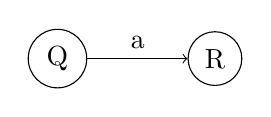
\begin{tikzpicture}
\node (Q) [circle,draw] at (0,1) {Q};
\node (R) [circle,draw] at (2,1) {R};
\draw [->] (Q) -- (R) node[midway,above] {a};
\end{tikzpicture}
\end{center}

\item<2-> Regular expression is needed for the part of the word that takes the machine from \texttt{Q} to \texttt{R}

\item<2-> A singleton regular expression is needed for the rule \texttt{(Q a R)}:
\begin{alltt}
     (singleton-regexp "a")
\end{alltt}

\end{itemize}
\end{scriptsize}
\end{frame}

\begin{frame}[fragile]
\frametitle{FSA and Regular Expressions}
%\framesubtitle{HOMEWORK}
\begin{scriptsize}
\begin{itemize}
\item<1-> There can be more than one transition from \texttt{Q} to \texttt{R}:
\begin{center}
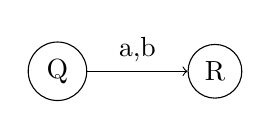
\begin{tikzpicture}
\node (Q) [circle,draw] at (0,1) {Q};
\node (R) [circle,draw] at (2,1) {R};
\draw [->] (Q) -- (R) node[midway,above] {a,b};
\end{tikzpicture}
\end{center}

\item<2-> The machine can move from \texttt{Q} to \texttt{R} on a \texttt{a} or on a \texttt{b}

\item<3-> A \texttt{union-regexp} is needed:
\begin{alltt}
     (union-regexp (singleton-regexp "a")
                   (singleton-regexp "b"))
\end{alltt}

\end{itemize}
\end{scriptsize}
\end{frame}

\begin{frame}[fragile]
\frametitle{FSA and Regular Expressions}
%\framesubtitle{HOMEWORK}
\begin{scriptsize}
\begin{itemize}
\item<1-> More than two connected nodes:
\begin{center}
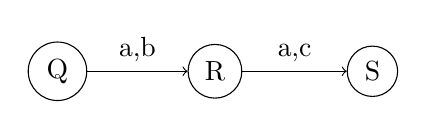
\begin{tikzpicture}
\node (Q) [circle,draw] at (0,1) {Q};
\node (R) [circle,draw] at (2,1) {R};
\node (S) [circle,draw] at (4,1) {S};
\draw [->] (Q) -- (R) node[midway,above] {a,b};
\draw [->] (R) -- (S) node[midway,above] {a,c};
\end{tikzpicture}
\end{center}

\item<1-> \texttt{S} is reachable from \texttt{Q}

\item<1-> A regular expression is needed to generate the part of the word that is consumed when the machine moves from \texttt{Q} to \texttt{S}

\item<2->
\begin{center}
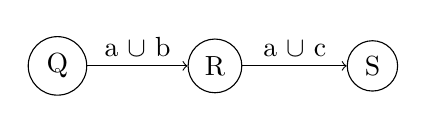
\begin{tikzpicture}
\node (Q) [circle,draw] at (0,1) {Q};
\node (R) [circle,draw] at (2,1) {R};
\node (S) [circle,draw] at (4,1) {S};
\draw [->] (Q) -- (R) node[midway,above] {a $\cup$ b};
\draw [->] (R) -- (S) node[midway,above] {a $\cup$ c};
\end{tikzpicture}
\end{center}

\item<3-> \texttt{R} may be ripped out, along with the transitions into and out of it

\item<3-> Substitute with a transition from \texttt{Q} to \texttt{S} that concatenates the regular expressions:
\begin{center}
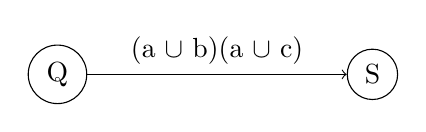
\begin{tikzpicture}
\node (Q) [circle,draw] at (0,1) {Q};
\node (S) [circle,draw] at (4,1) {S};
\draw [->] (Q) -- (S) node[midway,above] {(a $\cup$ b)(a $\cup$ c)};
\end{tikzpicture}
\end{center}

\item<4-> The needed regular expression:
\begin{alltt}
     (concat-regexp (union-regexp (singleton-regexp a)
                                  (singleton-regexp b))
                    (union-regexp (singleton-regexp a)
                                  (singleton-regexp c))
\end{alltt}


\end{itemize}
\end{scriptsize}
\end{frame}

\begin{frame}[fragile]
\frametitle{FSA and Regular Expressions}
%\framesubtitle{HOMEWORK}
\begin{scriptsize}
\begin{itemize}
\item<1-> The intermediate node \texttt{R} may have an loop on it:
\begin{center}
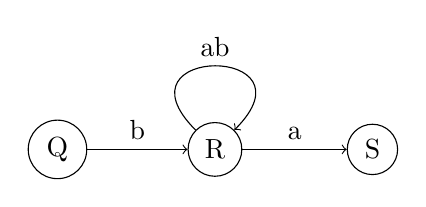
\begin{tikzpicture}
\node (Q) [circle,draw] at (0,1) {Q};
\node (R) [circle,draw] at (2,1) {R};
\node (S) [circle,draw] at (4,1) {S};
\draw [->] (Q) -- (R) node[midway,above] {b};
\draw [->] (R) -- (S) node[midway,above] {a};
\draw [->] (R) to [out=135,in=45,looseness=8] node[above] {ab} (R);
\end{tikzpicture}
\end{center}

\item<2-> To rip out the intermediate state the regular expression must generate the part of the word that takes the machine from \texttt{Q} to \texttt{R}, then generates zero or more times the part of the word that takes the machine from \texttt{R} to \texttt{R}, and finally generates the part of the word that takes the machine from \texttt{R} to \texttt{S}

\item<2-> A Kleene star regular expression is needed:
\begin{center}
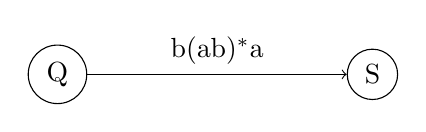
\begin{tikzpicture}
\node (Q) [circle,draw] at (0,1) {Q};
\node (S) [circle,draw] at (4,1) {S};
\draw [->] (Q) -- (S) node[midway,above] {b(ab)$^*$a};
\end{tikzpicture}
\end{center}

\item<3-> The needed regular expression is:
\begin{alltt}
     (concat-regexp
       (singleton-regexp "b")
       (concat-regexp
         (kleenestar-regexp
           (concat-regexp (singleton-regexp "a")
                          (singleton-regexp "b")))
         (singleton-regexp "a")))
\end{alltt}

\end{itemize}
\end{scriptsize}
\end{frame}

\begin{frame}[fragile]
\frametitle{FSA and Regular Expressions}
%\framesubtitle{HOMEWORK}
\begin{scriptsize}
\begin{itemize}
\item<1-> Given an \ndfa{} the goal is to construct a regular expression for all transition diagram paths from the start state to all reachable final states

\item<2-> Create a directed graph and rip out all the states

\item<2-> Initial digraph has all the machine's states as nodes and the edges are labeled with a regular expression for what is consumed by a transition between two states

\item<3-> In addition, the initial directed graph has two extra nodes representing a new start state and a new and only final state

\item<3-> There is an \et{} from the new start state to the machine's start state and there are \ets{} from every machine final state to the new final state

\item<4-> The process starts by collapsing multiple edges between two nodes into one labeled with a union regular expression

\item<4-> At each step, this graph is collapsed by ripping out a node

\item<5-> Ripping out a state may result in multiple edges between nodes and these are collapsed before moving on

\item<6-> After all machine states are ripped out the graph has been collapsed to two states (the new start state and the new final state) with a single edge between them

\item<6-> The label on that edge is the regular expression for the machine's language

\end{itemize}
\end{scriptsize}
\end{frame}

\begin{frame}[fragile]
\frametitle{FSA and Regular Expressions}
%\framesubtitle{HOMEWORK}
\begin{scriptsize}
\begin{itemize}
\item<1-> To rip out a state, \texttt{S}, the graph's edges are partitioned into 4 subsets:
\begin{quote}
\begin{description}
  \item[\texttt{not-s-edges}] The list of edges that are not into nor out of \texttt{S}
  \item[\texttt{into-s-edges}] The list of non-loop edges that are into \texttt{S}
  \item[\texttt{outof-s-edges}] The list of non-loop edges that are out of \texttt{S}
  \item[\texttt{self-edges}] The list of self-loop edges on \texttt{S}
\end{description}
\end{quote}

\item<2-> A new graph is constructed using \texttt{not-s-edges} and the new edges created using the other 3 sets of edges

\item<2-> If \texttt{S} has a self-loop new edges are created for each incoming edge using the outgoing edges

\item<2-> Each new edge is from the start node of the incoming node to the destination node of an outgoing edge

\item<2-> The edge's label is a concatenation regular expression for the label of the incoming edge, the Kleene star of the self-loop label, and the label of an outgoing edge

\item<3-> If \texttt{S} does not have a self-loop new edges are also created for each incoming edge using the outgoing edges

\item<3-> Each new edge is from the start node of the incoming node to the destination node of an outgoing edge

\item<3-> The edge's label is a concatenation regular expression for the label of the incoming edge and the label of an outgoing edge

\end{itemize}
\end{scriptsize}
\end{frame}

\begin{frame}[fragile]
\frametitle{FSA and Regular Expressions}
%\framesubtitle{HOMEWORK}
\begin{scriptsize}
\begin{itemize}
\item<1->
\begin{center}
\includegraphics[scale=0.4]{ndfa2regexp-ex.png}
\end{center}

\item<2-> Initial Graph collapse multiple edges between nodes:
\begin{center}
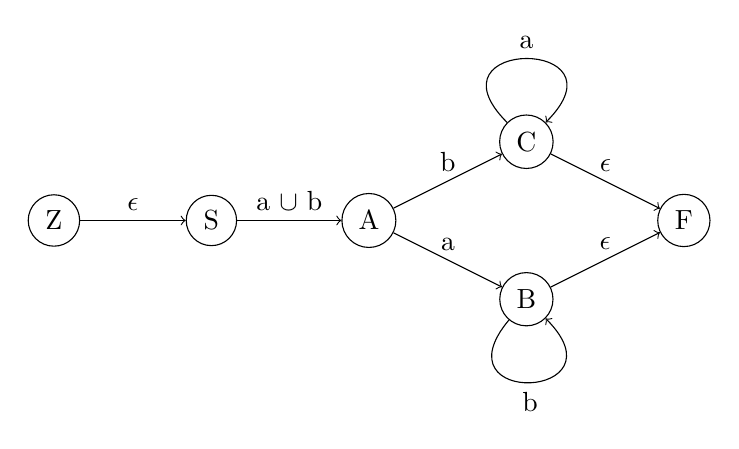
\begin{tikzpicture}
\node (Z) [circle,draw] at (0,1) {Z};
\node (S) [circle,draw] at (2,1) {S};
\node (A) [circle,draw] at (4,1) {A};
\node (B) [circle,draw] at (6,0) {B};
\node (C) [circle,draw] at (6,2) {C};
\node (F) [circle,draw] at (8,1) {F};
\draw [->] (Z) -- (S) node[midway,above] {$\epsilon$};
\draw [->] (S) -- (A) node[midway,above] {a $\cup$ b};
\draw [->] (A) -- (C) node[midway,above] {b};
\draw [->] (A) -- (B) node[midway,above] {a};
\draw [->] (C) to [out=135,in=45,looseness=8] node[above] {a} (C);
\draw [->] (B) to [out=-130,in=-45,looseness=8] node[below] {b} (B);
\draw [->] (C) -- (F) node[midway,above] {$\epsilon$};
\draw [->] (B) -- (F) node[midway,above] {$\epsilon$};
\end{tikzpicture}
\end{center}

\end{itemize}
\end{scriptsize}
\end{frame}

\begin{frame}[fragile]
\frametitle{FSA and Regular Expressions}
%\framesubtitle{HOMEWORK}
\begin{scriptsize}
\begin{itemize}
\item<1->
\begin{center}
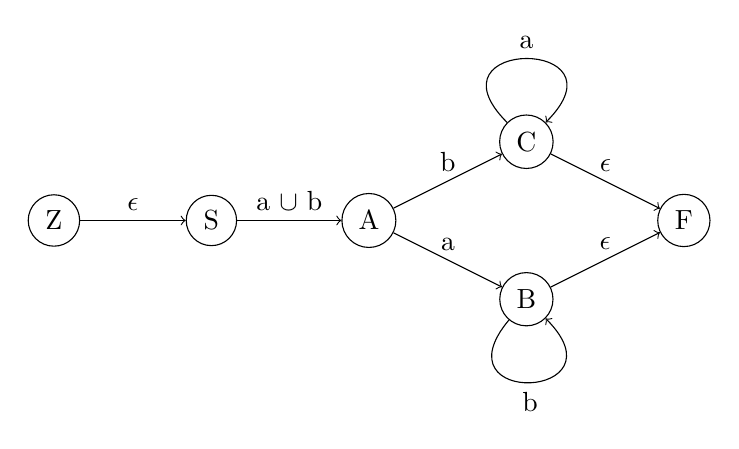
\begin{tikzpicture}
\node (Z) [circle,draw] at (0,1) {Z};
\node (S) [circle,draw] at (2,1) {S};
\node (A) [circle,draw] at (4,1) {A};
\node (B) [circle,draw] at (6,0) {B};
\node (C) [circle,draw] at (6,2) {C};
\node (F) [circle,draw] at (8,1) {F};
\draw [->] (Z) -- (S) node[midway,above] {$\epsilon$};
\draw [->] (S) -- (A) node[midway,above] {a $\cup$ b};
\draw [->] (A) -- (C) node[midway,above] {b};
\draw [->] (A) -- (B) node[midway,above] {a};
\draw [->] (C) to [out=135,in=45,looseness=8] node[above] {a} (C);
\draw [->] (B) to [out=-130,in=-45,looseness=8] node[below] {b} (B);
\draw [->] (C) -- (F) node[midway,above] {$\epsilon$};
\draw [->] (B) -- (F) node[midway,above] {$\epsilon$};
\end{tikzpicture}
\end{center}

\item<1-> To collapse the graph, at each step a node is ripped out

\item<1-> The order in which they are ripped out does not matter

\item<2-> Let us start by ripping out \texttt{C}:
\begin{center}
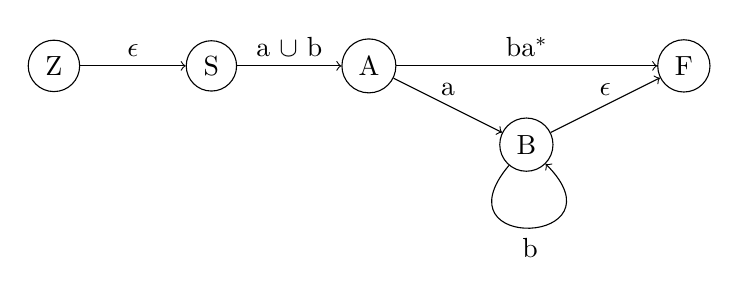
\begin{tikzpicture}
\node (Z) [circle,draw] at (0,1) {Z};
\node (S) [circle,draw] at (2,1) {S};
\node (A) [circle,draw] at (4,1) {A};
\node (B) [circle,draw] at (6,0) {B};
\node (F) [circle,draw] at (8,1) {F};
\draw [->] (Z) -- (S) node[midway,above] {$\epsilon$};
\draw [->] (S) -- (A) node[midway,above] {a $\cup$ b};
\draw [->] (A) -- (B) node[midway,above] {a};
\draw [->] (B) to [out=-130,in=-45,looseness=8] node[below] {b} (B);
\draw [->] (B) -- (F) node[midway,above] {$\epsilon$};
\draw [->] (A) -- (F) node[midway,above] {ba$^{*}$};
\end{tikzpicture}
\end{center}

\end{itemize}
\end{scriptsize}
\end{frame}

\begin{frame}[fragile]
\frametitle{FSA and Regular Expressions}
%\framesubtitle{HOMEWORK}
\begin{scriptsize}
\begin{itemize}

\item<1->
\begin{center}
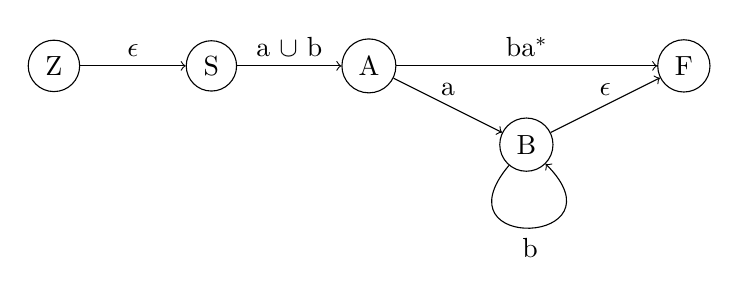
\begin{tikzpicture}
\node (Z) [circle,draw] at (0,1) {Z};
\node (S) [circle,draw] at (2,1) {S};
\node (A) [circle,draw] at (4,1) {A};
\node (B) [circle,draw] at (6,0) {B};
\node (F) [circle,draw] at (8,1) {F};
\draw [->] (Z) -- (S) node[midway,above] {$\epsilon$};
\draw [->] (S) -- (A) node[midway,above] {a $\cup$ b};
\draw [->] (A) -- (B) node[midway,above] {a};
\draw [->] (B) to [out=-130,in=-45,looseness=8] node[below] {b} (B);
\draw [->] (B) -- (F) node[midway,above] {$\epsilon$};
\draw [->] (A) -- (F) node[midway,above] {ba$^{*}$};
\end{tikzpicture}
\end{center}

\item<1-> Let us now rip out \texttt{B}:
\begin{center}
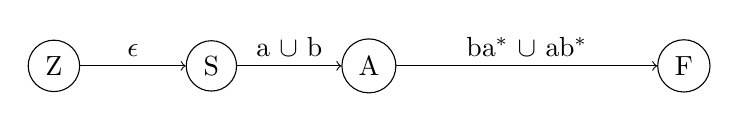
\begin{tikzpicture}
\node (Z) [circle,draw] at (0,1) {Z};
\node (S) [circle,draw] at (2,1) {S};
\node (A) [circle,draw] at (4,1) {A};
\node (F) [circle,draw] at (8,1) {F};
\draw [->] (Z) -- (S) node[midway,above] {$\epsilon$};
\draw [->] (S) -- (A) node[midway,above] {a $\cup$ b};
\draw [->] (A) -- (F) node[midway,above] {ba$^{*}$ $\cup$ ab$^{*}$};
\end{tikzpicture}
\end{center}

\end{itemize}
\end{scriptsize}
\end{frame}

\begin{frame}[fragile]
\frametitle{FSA and Regular Expressions}
%\framesubtitle{HOMEWORK}
\begin{scriptsize}
\begin{itemize}
\item<1->
\begin{center}
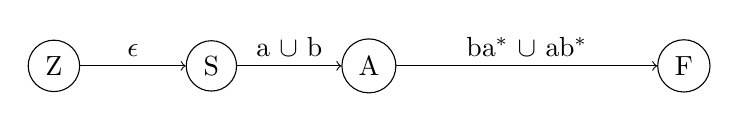
\begin{tikzpicture}
\node (Z) [circle,draw] at (0,1) {Z};
\node (S) [circle,draw] at (2,1) {S};
\node (A) [circle,draw] at (4,1) {A};
\node (F) [circle,draw] at (8,1) {F};
\draw [->] (Z) -- (S) node[midway,above] {$\epsilon$};
\draw [->] (S) -- (A) node[midway,above] {a $\cup$ b};
\draw [->] (A) -- (F) node[midway,above] {ba$^{*}$ $\cup$ ab$^{*}$};
\end{tikzpicture}
\end{center}

\item<1-> Let's rip out \texttt{S}:
\begin{center}
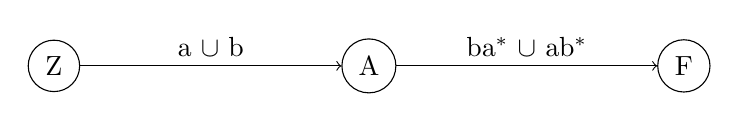
\begin{tikzpicture}
\node (Z) [circle,draw] at (0,1) {Z};
\node (A) [circle,draw] at (4,1) {A};
\node (F) [circle,draw] at (8,1) {F};
\draw [->] (Z) -- (A) node[midway,above] {a $\cup$ b};
\draw [->] (A) -- (F) node[midway,above] {ba$^{*}$ $\cup$ ab$^{*}$};
\end{tikzpicture}
\end{center}

\end{itemize}
\end{scriptsize}
\end{frame}

\begin{frame}[fragile]
\frametitle{FSA and Regular Expressions}
%\framesubtitle{HOMEWORK}
\begin{scriptsize}
\begin{itemize}
\item<1->
\begin{center}
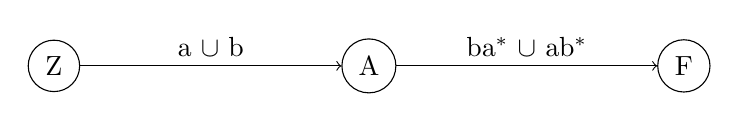
\begin{tikzpicture}
\node (Z) [circle,draw] at (0,1) {Z};
\node (A) [circle,draw] at (4,1) {A};
\node (F) [circle,draw] at (8,1) {F};
\draw [->] (Z) -- (A) node[midway,above] {a $\cup$ b};
\draw [->] (A) -- (F) node[midway,above] {ba$^{*}$ $\cup$ ab$^{*}$};
\end{tikzpicture}
\end{center}

\item<1-> Let's rip out \texttt{A}:
\begin{center}
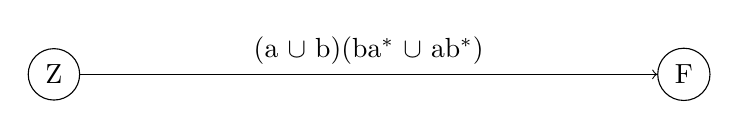
\begin{tikzpicture}
\node (Z) [circle,draw] at (0,1) {Z};
\node (F) [circle,draw] at (8,1) {F};
\draw [->] (Z) -- (F) node[midway,above] {(a $\cup$ b)(ba$^{*}$ $\cup$ ab$^{*}$)};
\end{tikzpicture}
\end{center}

\end{itemize}
\end{scriptsize}
\end{frame}

\begin{frame}[fragile]
\frametitle{FSA and Regular Expressions}
%\framesubtitle{HOMEWORK}
\begin{scriptsize}
\begin{itemize}
\item<1->
\begin{center}
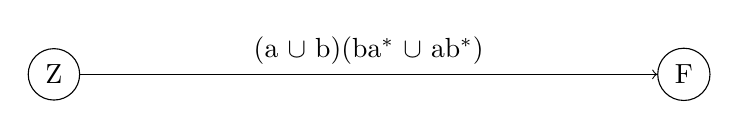
\begin{tikzpicture}
\node (Z) [circle,draw] at (0,1) {Z};
\node (F) [circle,draw] at (8,1) {F};
\draw [->] (Z) -- (F) node[midway,above] {(a $\cup$ b)(ba$^{*}$ $\cup$ ab$^{*}$)};
\end{tikzpicture}
\end{center}

\item<1-> All nodes for machine states ripped out

\item<2->
\begin{alltt}
     (concat-regexp
       (union-regexp (singleton-regexp "a")
                     (singleton-regexp "b"))
       (union-regexp
         (concat-regexp
           (singleton-regexp "b")
           (kleenestar-regexp (singleton-regexp "a")))
         (concat-regexp
           (singleton-regexp "a")
           (kleenestar-regexp (singleton-regexp "b")))))
\end{alltt}

\end{itemize}
\end{scriptsize}
\end{frame}

\begin{frame}[fragile]
\frametitle{FSA and Regular Expressions}
%\framesubtitle{HOMEWORK}
\begin{scriptsize}
\begin{itemize}
\item<1-> The discussion so far has assumed that \texttt{L(M) $\neq$ $\varnothing$}

\item<2-> If the language of the given machine is empty then the collapsed graph will have no edges

\item<2-> This is a problem because there is no regular expression for generating no words

\item<3-> To address this problem \fsm{} introduces a new regular expression constructor, \texttt{null-regexp}, to represent a language with no words
    
\item<3-> Illustrate ndfa2regexp-viz using ndfa2regexp.rkt

\end{itemize}
\end{scriptsize}
\end{frame}

\begin{frame}[fragile]
\frametitle{FSA and Regular Expressions}
%\framesubtitle{HOMEWORK}
\begin{scriptsize}
\begin{itemize}
\item<1->
\begin{alltt}
     ;; Data Definitions
     ;;
     ;; A node is a symbol
     ;;
     ;; An edge, (list node regexp node), has a beginning
     ;; node, a regular expression for its label, and
     ;; destination node.
     ;;
     ;; A directed graph, dgraph, is a (listof edge)
\end{alltt}

\end{itemize}
\end{scriptsize}
\end{frame}

\begin{frame}[fragile]
\frametitle{FSA and Regular Expressions}
%\framesubtitle{HOMEWORK}
\begin{scriptsize}
\begin{itemize}
\item<1-> To test the constructor \texttt{EVEN-A-ODD-B} and the following machines are used:
\begin{alltt}
  ;; L = {}
  (define EMPTY (make-ndfa \quot{}(S) \quot{}(a b) \quot{}S \elist \elist))

  ;; L = ab* U ba*
  (define aUb-ba*Uab*
         (make-ndfa
           \quot{}(S A B C)
           \quot{}(a b)
           \quot{}S
           \quot{}(B C)
           \quot{}((S a A) (S b A) (A a B) (A b C) (B b B) (C a C))))

  ;; L = b*
  (define b* (make-ndfa \qquot(,DEAD S A)
                        \quot{}(a b)
                        \quot{}S
                        \quot{}(A)
                        \qquot{}((S ,EMP A) (S a ,DEAD) (A b A))))
\end{alltt}

\end{itemize}
\end{scriptsize}
\end{frame}

\begin{frame}[fragile]
\frametitle{FSA and Regular Expressions}
%\framesubtitle{HOMEWORK}
\begin{tiny}
\begin{itemize}
\item<1->
\begin{alltt}
;; ndfa \arrow regexp  Purpose: Create a regexp from the given ndfa
;; Assume: Transition diagram of machine is connected digraph
(define (ndfa2regexp m)
\end{alltt}

\item<3->
\begin{alltt}
  (let* [(new-start (generate-symbol \quot{}S (sm-states m)))
\end{alltt}

\item<4->
\begin{alltt}
         (new-final (generate-symbol \quot{}F (sm-states m)))
\end{alltt}

\item<5->
\begin{alltt}
         (init-dgraph (make-dgraph
                       (cons (list new-start EMP (sm-start m))
                             (append
                              (map (\lamb (f) (list f EMP new-final))
                                     (sm-finals m))
                                   (sm-rules m)))))
\end{alltt}

\item<6->
\begin{alltt}
         (collapsed-dgraph
          (rip-out-nodes (sm-states m)
                         (remove-multiple-edges init-dgraph)))]
\end{alltt}

\item<7->
\begin{alltt}
    (if (empty? collapsed-dgraph)
        (null-regexp)
        (simplify-regexp (second (first collapsed-dgraph))))))
\end{alltt}

\item<2->
\begin{alltt}
;; Tests for ndfa2regexp
(check-equal? (printable-regexp (ndfa2regexp EMPTY)) "()")
(check-equal? (printable-regexp (ndfa2regexp b*))    "b*")
(check-equal? (printable-regexp (ndfa2regexp ab*Uaa*)) "(b U a)(ab* U ba*)")
\textcolor{red}{Alternative testing (for messy regexps)}
(define EVEN-A-ODD-B-regexp (ndfa2regexp EVEN-A-ODD-B))
(check-equal?
 (sm-apply EVEN-A-ODD-B (gen-regexp-word EVEN-A-ODD-B-regexp))
 'accept)
(check-equal?
 (sm-apply EVEN-A-ODD-B (gen-regexp-word EVEN-A-ODD-B-regexp))
 'accept)
(check-equal?
 (sm-apply EVEN-A-ODD-B (gen-regexp-word EVEN-A-ODD-B-regexp))
 'accept)
\end{alltt}

\end{itemize}
\end{tiny}
\end{frame}

\begin{frame}[fragile]
\frametitle{FSA and Regular Expressions}
%\framesubtitle{HOMEWORK}
\begin{scriptsize}
\begin{itemize}
\item<1->
\begin{alltt}
   ;; (listof ndfa-rule) \arrow dgraph
   ;; Purpose: Create a dgraph from the given ndfa
   (define (make-dgraph lor)
\end{alltt}

\item<3->
\begin{alltt}
     (map (\lamb (r) (if (eq? (second r) EMP)
                     (list (first r) (empty-regexp) (third r))
                     (list (first r)
                           (singleton-regexp (symbol->string (second r)))
                           (third r))))
          lor))
\end{alltt}

\item<2->
\begin{alltt}
   ;; Tests for make-dgraph
   (check-equal? (make-dgraph \elist) \elist)

   (check-equal?
    (make-dgraph \qquot{}((S ,EMP A) (S a ,DEAD) (A b A)))
    (list (list \quot{}S (empty-regexp) \quot{}A)
          (list \quot{}S (singleton-regexp "a") \quot{}ds)
          (list \quot{}A (singleton-regexp "b") \quot{}A)))

   (check-equal?
    (make-dgraph \quot{}((S a A) (S b A) (A a B) (A b C) (B b B) (C a C)))
    (list (list \quot{}S (singleton-regexp "a") \quot{}A)
          (list \quot{}S (singleton-regexp "b") \quot{}A)
          (list \quot{}A (singleton-regexp "a") \quot{}B)
          (list \quot{}A (singleton-regexp "b") \quot{}C)
          (list \quot{}B (singleton-regexp "b") \quot{}B)
          (list \quot{}C (singleton-regexp "a") \quot{}C)))
\end{alltt}

\end{itemize}
\end{scriptsize}
\end{frame}

\begin{frame}[fragile]
\frametitle{FSA and Regular Expressions}
%\framesubtitle{HOMEWORK}
\begin{scriptsize}
\begin{itemize}
\item<1->
\begin{alltt}
;; dgraph \arrow dgraph
;; Purpose: Collapse multiple edges between nodes
;; Accumulator Invariant: g = the unprocessed graph
(define (remove-multiple-edges g)
\end{alltt}

\item<3->
\begin{alltt}
  (if (empty? g)
      \elist
\end{alltt}

\item<4->
\begin{alltt}
      (let* [(curr-edge (first g))
             (from-state (first curr-edge))
             (to-state (third curr-edge))
             (to-collapse (filter (\lamb (e) (and (eq? (first e) from-state)
                                              (eq? (third e) to-state)))
                                  g))
             (remaining-g (filter (\lamb (e) (not (member e to-collapse))) g))]
        (cons (list from-state (collapse-edges to-collapse) to-state)
              (remove-multiple-edges remaining-g)))))
\end{alltt}

\item<2->
\begin{alltt}
;; Tests for remove-multiple-edges
(check-equal? \elist \elist)
(check-equal?
 (remove-multiple-edges \qquot((S ,(singleton-regexp "a") A)
                          (S ,(singleton-regexp "b") A)
                          (A ,(singleton-regexp "a") A)))
 \qquot((S
    ,(union-regexp (singleton-regexp "a") (singleton-regexp "b"))
    A)
   (A ,(singleton-regexp "a") A)))
\end{alltt}

\end{itemize}
\end{scriptsize}
\end{frame}

\begin{frame}[fragile]
\frametitle{FSA and Regular Expressions}
%\framesubtitle{HOMEWORK}
\begin{scriptsize}
\begin{itemize}
\item<1->
\begin{alltt}
;; (listof edge) \arrow regexp
;; Purpose: Collapse the given edges into a regexp
(define (collapse-edges loe)
  (cond [(empty? loe) \elist]
        [(empty? (rest loe)) (second (first loe))]
        [else (union-regexp (second (first loe))
                            (collapse-edges (rest loe)))]))
;; Tests for collapse-edges
(check-equal? (collapse-edges \elist) \elist)
(check-equal? (collapse-edges \qquot{}((S ,(singleton-regexp "a") S)))
              (singleton-regexp "a"))
(check-equal?
 (collapse-edges \qquot{}((A ,(singleton-regexp "a") A)
                   (A ,(singleton-regexp "b") A)
                   (A ,(empty-regexp) A)))
 (union-regexp (singleton-regexp "a")
               (union-regexp (singleton-regexp "b")
                             (empty-regexp))))
\end{alltt}

\end{itemize}
\end{scriptsize}
\end{frame}

\begin{frame}[fragile]
\frametitle{FSA and Regular Expressions}
%\framesubtitle{HOMEWORK}
\begin{scriptsize}
\begin{itemize}
\item<1->
\begin{alltt}
;; (listof node) dgraph \arrow dgraph
;; Purpose: Rip out the given nodes from the given graph
;; Assume: Given nodes in given graph and g has no multiple edges
;;         between nodes
(define (rip-out-nodes lon g)
  (foldr (\lamb (s g) (rip-out-node s g)) g lon))

;; Tests for rip-out-nodes
(check-equal? (rip-out-nodes \elist \qquot{}((S ,(singleton-regexp "a") A)
                               (A ,(singleton-regexp "b") B)))
              \qquot{}((S ,(singleton-regexp "a") A)
                (A ,(singleton-regexp "b") B)))

(check-equal?
  (rip-out-nodes \quot{}(A B) \qquot{}((S ,(singleton-regexp "a") A)
                          (A ,(singleton-regexp "b") B)
                          (B ,(singleton-regexp "b") C)))
  \qquot{}((S
    ,(concat-regexp (singleton-regexp "a")
                    (concat-regexp (singleton-regexp "b")
                                   (singleton-regexp "b")))
    C)))
\end{alltt}

\end{itemize}
\end{scriptsize}
\end{frame}

\begin{frame}[fragile]
\frametitle{FSA and Regular Expressions}
%\framesubtitle{HOMEWORK}
\begin{scriptsize}
\begin{itemize}
\item<1->
\begin{alltt}
;; state dgraph \arrow dgraph    Purpose: Rip out given node from given graph
;; Assume: Given node in given graph and g has no multiple edges between nodes
(define (rip-out-node n g)
\end{alltt}

\end{itemize}
\end{scriptsize}
\end{frame}

\begin{frame}[fragile]
\frametitle{FSA and Regular Expressions}
%\framesubtitle{HOMEWORK}
\begin{scriptsize}
\begin{itemize}
\item<1->
\begin{alltt}
;; Tests for rip-out-node
(check-equal?
 (rip-out-node
   \quot{}A
   \qquot{}((S ,(singleton-regexp "a") A) (A ,(singleton-regexp "b") B)))
 \qquot{}((S
           ,(concat-regexp (singleton-regexp "a") (singleton-regexp "b"))
           B)))
(check-equal?
  (rip-out-node
    \quot{}C
    \qquot{}((S ,(singleton-regexp "a") A) (S ,(singleton-regexp "b") B)
      (A ,(singleton-regexp "a") C) (B ,(singleton-regexp "b") C)
      (C ,(singleton-regexp "a") D) (C ,(singleton-regexp "b") E)))
  \qquot{}((S ,(singleton-regexp "a") A)
    (S ,(singleton-regexp "b") B)
    (A
     ,(concat-regexp (singleton-regexp "a") (singleton-regexp "a"))
     D)
    (A
     ,(concat-regexp (singleton-regexp "a") (singleton-regexp "b"))
     E)
    (B ,(concat-regexp (singleton-regexp "b") (singleton-regexp "a")) D)
    (B ,(concat-regexp (singleton-regexp "b") (singleton-regexp "b")) E)))
\end{alltt}

\end{itemize}
\end{scriptsize}
\end{frame}

\begin{frame}[fragile]
\frametitle{FSA and Regular Expressions}
%\framesubtitle{HOMEWORK}
\begin{tiny}
\begin{itemize}
\item<1->
\begin{alltt}
;; state dgraph \arrow dgraph Purpose: Rip out given node from given graph
;; Assume: Given node in given graph and g has no multiple edges between nodes
(define (rip-out-node n g)
 (let*
  [(non (filter (\lamb (r) (and (not (eq? (third r) n))(not (eq? (first r) n)))) g))
 \end{alltt}

\item<2->
\begin{alltt}
   (into-n (filter (\lamb (r) (and (eq? (third r) n) (not (eq? (first r) n)))) g))
\end{alltt}

\item<3->
\begin{alltt}
   (outof-n (filter (\lamb (r) (and (eq? (first r) n) (not (eq? (third r) n)))) g))
\end{alltt}

\item<4->
\begin{alltt}
   (self-edges (filter (\lamb (r) (and (eq? (first r) n) (eq? (third r) n))) g))]

 (remove-multiple-edges
     (append
      non
\end{alltt}

\item<5->
\begin{alltt}
      (if (not (empty? self-edges))
          (let [(se (first self-edges))]
            (append-map
              (\lamb (into-edge)
                (map (\lamb (outof-edge)
                       (list (first into-edge)
                             (concat-regexp
                               (second into-edge)
                               (concat-regexp (kleenestar-regexp (second se))
                                              (second outof-edge)))
                             (third outof-edge)))
                     outof-s-edges))
              into-s-edges))
\end{alltt}

\item<6->
\begin{alltt}
          (append-map
            (\lamb (into-edge)
              (map (\lamb (outof-edge) (list (first into-edge)
                                         (concat-regexp (second into-edge)
                                                        (second outof-edge))
                                         (third outof-edge)))
                   outof-s-edges))
            into-s-edges))))))
\end{alltt}

\end{itemize}
\end{tiny}
\end{frame}

\begin{frame}[fragile]
\frametitle{FSA and Regular Expressions}
%\framesubtitle{HOMEWORK}
\begin{scriptsize}
\begin{theorem}
(ndfa2regexp m) returns a regular expression for L(m).
\end{theorem}

\begin{itemize}
\item<1-> The proof of correctness requires proving that all functions return the expected value

\item<1-> To prove that each function is correct assume that the auxiliary functions are correct

\item<1-> We start with the main function

\end{itemize}
\end{scriptsize}
\end{frame}

\begin{frame}[fragile]
\frametitle{FSA and Regular Expressions}
%\framesubtitle{HOMEWORK}
\begin{scriptsize}
\begin{theorem}
(ndfa2regexp m) returns a regular expression for L(m).
\end{theorem}

\begin{itemize}
\item<1-> New start and final states are generated

\item<1-> To m's rules \ets{} are added from the new start state to m's start state and from each of m's final states to the new final state

\item<2-> By assumption, \texttt{make-dgraph} creates the correct initial directed graph

\item<2-> Multiple edges between any pair of nodes are removed by \texttt{remove-multiple-edges}

\item<2-> All the nodes that represent a state in m are ripped out by \texttt{rip-out-nodes} to create the collapsed graph

\item<3-> Observe that the graph meets the assumptions made by \texttt{rip-out-nodes}

\item<3-> These auxiliary functions, by assuming their correctness, return the correct graph for their given input

\item<4-> The collapsed graph is examined to test if it is empty

\item<4-> If so, \texttt{(null-regexp)} is returned because L(m) is empty

\item<5-> Otherwise, the only edge's regular expression is returned

\item<5-> This is correct because this regular expression can generate words on all paths from the new start state to the new final state in the initial directed graph

\end{itemize}
\end{scriptsize}
\end{frame}

\begin{frame}[fragile]
\frametitle{FSA and Regular Expressions}
%\framesubtitle{HOMEWORK}
\begin{scriptsize}
\begin{theorem}
(rip-out-nodes lon g) returns a dgraph resulting from removing the given nodes from the given graph.
\end{theorem}

\begin{itemize}
\item<1-> By assumption, all the given nodes are in the given graph and the given graph does not have multiple edges between nodes

\item<2-> The given list of nodes is traversed using \texttt{foldr} to rip out one node at a time

\item<2-> Initially, \texttt{foldr}'s accumulator is the given graph

\item<2-> For each node, \texttt{foldr} creates a new graph by ripping out the next node using \texttt{rip-out-node}

\item<3-> Observe that the graph returned by \texttt{rip-out-node} satisfies the assumptions made by this function

\item<3-> Therefore, the returned graph may be input to \texttt{rip-out-node}

\item<3-> This auxiliary function, by assumption, is correct

\item<3-> Thus, \texttt{rip-out-nodes} returns the correct directed graph after ripping out all the given nodes

\end{itemize}
\end{scriptsize}
\end{frame}

\begin{frame}[fragile]
\frametitle{FSA and Regular Expressions}
%\framesubtitle{HOMEWORK}
\begin{tiny}
\begin{theorem}
(rip-out-node n g) returns a dgraph resulting from removing the given node from the given dgraph.
\end{theorem}

\begin{itemize}
\item<1-> By assumption, the given node is in the given graph

\item<2-> Extracts four mutually exclusive sets of rules:
\begin{description}
  \item[\texttt{non}] The set of edges that are not into nor out of n
  \item[\texttt{into-n}] The set of edges into n
  \item[\texttt{outof-n}] The set of edges out of n
  \item[\texttt{self-edges}] The set of edges that are self-loops on n $\leftarrow$ at most one
\end{description}

\item<3-> If there is a self-loop on n, for each edge, i, in \texttt{into-n} a new edge is created using each edge, o, in \texttt{outof-n} that has the following form:
\begin{alltt}
  (\emph{starting state of i}
   (concat-regexp
     \emph{regular expression in i}
     (concat-regexp
       (kleenestar-regexp \emph{regular expression in only self-edge})
       \emph{regular expression in o}))
   \emph{destination state of o})
\end{alltt}

\item<3-> This is correct because the regular expression can generate all words that take the machine from the state represented by the starting node of i to the destination state of o

\item<4-> If there is no self-loop on n then for each edge, i, in \texttt{into-n} a new edge is created using each edge, o, in \texttt{outof-n}:
\begin{alltt}
     (\emph{starting state of i}
      (concat-regexp
        \emph{regular expression in i}
        \emph{regular expression in o})
      \emph{destination state of o})
\end{alltt}

\item<4-> This is correct because the regular expression can generate all words that take the machine from the state represented by the starting node of i to the state represented by the destination node of o

\item<5-> The remaining proofs for auxiliary functions are left as exercises

\end{itemize}
\end{tiny}
\end{frame}

\begin{frame}[fragile]
\frametitle{FSA and Regular Expressions}
%\framesubtitle{HOMEWORK}
\begin{scriptsize}
\begin{itemize}
\item<1-> HOMEWORK: 17--19

\item<1-> QUIZ: 20 (due in a week)

\end{itemize}
\end{scriptsize}
\end{frame}


\section{Regular Grammars}

\begin{frame}[fragile]
\frametitle{Regular Grammars}
%\framesubtitle{HOMEWORK}
\begin{scriptsize}
\begin{itemize}
\item<1-> We know that a \dfa{} decides a regular language by reading one symbol at a time

\item<1-> This suggests that words in the language may be generated one symbol at a time starting with a symbol \texttt{S}

\item<2-> We have to be able to generate the empty word because it may be part of a regular language

\item<3-> There are three types of rules in a regular grammar:
\begin{quote}
\begin{enumerate}
 \item S generates the empty word (i.e., \texttt{EMP})
 \item Rules that generate an alphabet member
 \item Rules that generate a symbol representing the concatenation of a terminal symbol and a symbol representing a syntactic category.
\end{enumerate}
\end{quote}

\item<3-> The members of the alphabet are the terminal symbols

\item<3-> The symbols representing syntactic categories are the nonterminals

\end{itemize}
\end{scriptsize}
\end{frame}

\begin{frame}[fragile]
\frametitle{Regular Grammars}
%\framesubtitle{HOMEWORK}
\begin{scriptsize}
\begin{itemize}
\item<1-> Formally:
\begin{alltt}
     A regular grammar is an instance of (make-rg N \sig{} R S)
\end{alltt}

\item<1-> \texttt{N} is the set of capital letters in the Roman alphabet representing the nonterminal symbols

\item<1-> \sig{} is the set of lowercase symbols called the alphabet

\item<1-> \texttt{S} is the starting nonterminal symbol

\item<1-> \texttt{R} is the set of generating (or production) rules

\item<2-> Each production rule contains a nonterminal followed by an arrow and a symbol

\item<2-> There are only 3 types of production rules:
\begin{alltt}
     S \arrow \(\epsilon\), where S is the starting nonterminal and S\(\in\)N
     A \arrow a,  where A\(\in\)N and a\(\in\)\sig
     A \arrow aB, where A,B\(\in\)N and a\(\in\)\sig
\end{alltt}

\item<2-> Observe that each rule generates one terminal symbol at a time

\item<3-> The language of a grammar \texttt{G} is denoted as \texttt{L(G)}

\item<3-> It contains all the words that can be generated using \texttt{G}

\end{itemize}
\end{scriptsize}
\end{frame}

\begin{frame}[fragile]
\frametitle{Regular Grammars}
%\framesubtitle{HOMEWORK}
\begin{scriptsize}
\begin{itemize}
\item<1-> Grammar observers:
\begin{description}
  \item[\underline{\texttt{(grammar-nts g)}}:] Returns a list of \texttt{g}'s nonterminal symbols.
  \item[\underline{\texttt{(grammar-sigma g)}}:] Returns a list of \texttt{g}'s terminal symbols.
  \item[\underline{\texttt{(grammar-rules g)}}:] Returns a list of \texttt{g}'s production rules
  \item[\underline{\texttt{(grammar-start g)}}:] Returns \texttt{g}'s starting nonterminal.
  \item[\underline{\texttt{(grammar-type g)}}:] Returns a symbol for \texttt{g}'s grammar type.
  \item[\underline{\texttt{(grammar-derive g w)}}:] If the given word, \texttt{w}, is in the language of the given grammar then a derivation for \texttt{w} is returned. Otherwise, a string indicating that \texttt{w} is not in the language of the given grammar is returned.
\end{description}

\item<1-> A derivation consists of 1 or more derivation steps

\item<1-> A derivation step is denoted by \gstep{}

\item<1-> One or more derivation steps is denoted by \gsteps{}.

\item<2-> Testing functions:
\begin{description}
  \item[\underline{\texttt{(grammar-both-derive g1 g2 w)}}:] Tests if both of the given grammars derive the given word.
  \item[\underline{\texttt{(grammar-testequiv g1 g2 [natnum])}}:] Tests if the given grammars derive 100 (or the optional number of) randomly generated words. If all tests give the same result true is returned. Otherwise, a list or words that produce different results is returned.
  \item[\underline{\texttt{(grammar-test g1 [natnum])}}:] Tests the given grammar with 100 (or the optional number of) randomly generated words. A list of pairs containing a word and the result of attempting to derive the word are returned.
\end{description}

\end{itemize}
\end{scriptsize}
\end{frame}

\begin{frame}[fragile]
\frametitle{Regular Grammars}
%\framesubtitle{HOMEWORK}
\begin{scriptsize}
\begin{itemize}
\item<1-> The Design Recipe for Grammars
\begin{enumerate}
\item Pick a name for the grammar and specify the alphabet
\item Define each syntactic category and associate each with a nonterminal clearly specifying the starting nonterminal
\item Develop the production rules
\item Write unit tests
\item Implement the grammar
\item Run the tests and redesign if necessary
\item \textcolor{blue}{For each syntactic category design and implement an invariant predicate to determine if a given word satisfies the role of the syntactic category}
\item \textcolor{blue}{For words in \texttt{L(G)} prove that the invariant predicates hold for every derivation step}
\item \textcolor{blue}{Prove that \texttt{L} = \texttt{L(G)}}
\end{enumerate}

\end{itemize}
\end{scriptsize}
\end{frame}

\begin{frame}[fragile]
\frametitle{Regular Grammars}
%\framesubtitle{HOMEWORK}
\begin{scriptsize}
\begin{itemize}
\item<1-> Design a regular grammar for:
\begin{alltt}
     L = a\(\sp{*}\)
\end{alltt}

\item<2-> Design idea: Generate an arbitrary number of \texttt{a}s using a single nonterminal that eventually generates the empty word

\item<4-> 
\begin{alltt}
;; Syntactic categories documentation
;;  S generates words in a\(\sp{*}\), starting nonterminal
\end{alltt}

\item<3->
\begin{alltt}
(define A* 
  (make-rg
\end{alltt}

\item<4->
\begin{alltt}
           \quot{}(S)
\end{alltt}

\item<3->
\begin{alltt}
           \quot{}(a b)
\end{alltt}

\item<5->
\begin{alltt}
           \qquot{}((S ,ARROW ,EMP)
             (S ,ARROW aS))
\end{alltt}

\item<4->
\begin{alltt}
           \quot{}S
\end{alltt}

\item<6->
\begin{alltt}
           #:rejects \quot{}((b) (a a b) (b a b b a))
           #:accepts \quot{}(() (a) (a a a a a a) (a a a))))
\end{alltt}

\item<7-> \texttt{S} generates an arbitrary number of \texttt{a}s
\begin{alltt}
(define (S-INV w) (andmap (\lamb{} (l) (eq? l \quot{}a)) w))
\end{alltt}

\end{itemize}
\end{scriptsize}
\end{frame}

\begin{frame}[fragile]
\frametitle{Regular Grammars}
%\framesubtitle{HOMEWORK}
\begin{scriptsize}
\begin{itemize}
\item<1-> To prove that invariants holds for words in the grammar's language, we perform an induction on, h, the height of the derivation tree
    
\item<1-> Consider any derivation tree of height h that the grammar can generate

\item<2->
\begin{alltt}
Base Case: h=1
Derivation tree is generated using (S -> EMP). This 
means w=EMP. Thus, S-INV holds.
\end{alltt}

\item<3->
\begin{alltt}
Inductive Step
Assume: Invariants hold for a tree of height k
  Show: Invariants hold for a tree of height k+1
\end{alltt}

\item<4->
\begin{alltt}
k>=1 \(\Rightarrow\) k>1 \(\Rightarrow\) The derivation tree is generated using:
(S -> aS)
The height of the derivation tree for the S on the RHS has 
height <= k.  By IH, its  yield (i.e., what it generates) is 
in a\(\sp{\texttt{*}}\). This rule makes the yield for the S on the LHS aa*. 
Thus, S-INV holds. 
\end{alltt}

\end{itemize}
\end{scriptsize}
\end{frame}

\begin{frame}[fragile]
\frametitle{Regular Grammars}
%\framesubtitle{HOMEWORK}
\begin{tiny}
\begin{itemize}
\item<1-> To proof that the language of a grammar is correct. We prove two lemmas:
    \begin{enumerate}
      \item w$\in$L(G) $\Leftrightarrow$ w$\in$L
      \item w$\notin$L(G) $\Leftrightarrow$ w$\notin$L
    \end{enumerate}

\item<2-> L = a$^{\textrm{*}}$
\begin{alltt}
w\(\in\)L(A*) \(\Leftrightarrow\) w\(\in\)L
\end{alltt}

\item<3->
\begin{alltt}
w\(\in\)L(A*) \(\Rightarrow\) w\(\in\)L
(\(\Rightarrow\)) Assume w\(\in\)L(A*)
This means there is a derivation tree for w. Given that invariants 
always hold, w\(\in\)L.
\end{alltt}

\item<4->
\begin{alltt}
(\(\Leftarrow\)) Assume w\(\in\)L
This means w=EMP or w\(\in\)a\(\sp{i}\), where i>0

w=EMP
  The derivation tree is generated using (S -> EMP).
  Thus, w in L(A*). 
w\(\in\)a\(\sp{i}\), where i>0
  Given that invariants always hold, the derivation tree is 
  generated using (S -> aS). Thus, w\(\in\)L(A*).
\end{alltt}

\item<5->
\begin{alltt}

w\(\notin\)L(A*) \(\Leftrightarrow\) w\(\notin\)L
\end{alltt}

\item<6->
\begin{alltt}
(\(\Rightarrow\)) Assume w\(\notin\)L(A*)
This means there is no derivation tree for w. Assume z
is the longest suffix of w that only contains as. That is,
w=xsz, where x\(\in\){a b}* and s\(\in\){a b EMP}. Observe that
s=b and, therefore, w=xbz. Otherwise, our assumptions are
contradicted. Thus, w\(\notin\)L.
\end{alltt}

\item<7->
\begin{alltt}
(\(\Leftarrow\)) Assume w\(\notin\)L
This means w contains a b. Given that invariants always hold,
A* does not generate w. Thus, w\(\notin\)L(A*).
\end{alltt}

\end{itemize}
\end{tiny}
\end{frame}


\begin{frame}[fragile]
\frametitle{Regular Grammars}
%\framesubtitle{HOMEWORK}
\begin{tiny}
\begin{itemize}
\item<1-> Design a regular grammar for L = \{w$|$w has more \texttt{b}s than \texttt{a}s\}

\item<2-> Design idea: Generate a word with a number of \texttt{b}s $\geq$ number of \texttt{a}s, followed by a b, followed by a word with a number of \texttt{b}s $\geq$ number of \texttt{a}s
    
\item<2-> Observe that two different languages need to be generated

\item<4-> 
\begin{alltt}
;; Syntactic Category Documentation
;;  S: generates words with number of b > number of a, starting nonterminal
;;  A: generates words with number of b \(\geq\) number of a
\end{alltt}

\item<3->
\begin{alltt}
(define numb>numa 
  (make-cfg
\end{alltt}

\item<4->
\begin{alltt}
           \quot{}(S A)
\end{alltt}

\item<3->
\begin{alltt}
           \quot{}(a b)
\end{alltt}

\item<5->
\begin{alltt}
           \qquot{}((S -> b) (S -> AbA)
             (A -> EMP)      (A -> bA)
             (A -> AbAaA)    (A -> AaAbA) )
\end{alltt}

\item<4->
\begin{alltt}
           \quot{}S
\end{alltt}

\item<6->
\begin{alltt}
           #:rejects \quot{}((a b) (a b a) (a a a a a))
           #:accepts \quot{}((b b b) (b b a b a a b) (a a a b b b b))))
\end{alltt}

\item<7-> \texttt{S} generates an arbitrary number of \texttt{a}s
\begin{alltt}
(define (S-INV yield)
  (let [(as (filter (\lamb{} (s) (eq? s \quot{}a)) yield))
        (bs (filter (\lamb{} (s) (eq? s \quot{}b)) yield))]
    (> (length bs) (length as))))

(define (A-INV yield)
  (let [(as (filter (\lamb{} (s) (eq? s \quot{}a)) yield))
        (bs (filter (\lamb{} (s) (eq? s \quot{}b)) yield))]
    (>= (length bs) (length as))))
\end{alltt}

\end{itemize}
\end{tiny}
\end{frame}

\begin{frame}[fragile]
\frametitle{Regular Grammars}
%\framesubtitle{HOMEWORK}
\begin{tiny}
\begin{itemize}
\item<1-> L = \{w$|$w has more \texttt{b}s than \texttt{a}s\}

\item<2->
\begin{alltt}
Base Case: h=1

(S -> b)
Yield has more bs than as. S-INV holds.

(A -> EMP)
Yield has equal number of bs than as. A-INV holds.
\end{alltt}

\item<3->
\begin{alltt}
Inductive Step
Assume: Invariants hold for a tree of height k
  Show: Invariants hold for a tree of height k+1

k>=1 \(\Rightarrow\) k>1 \(\Rightarrow\) The derivation tree is generated using:
\end{alltt}

\item<4->
\begin{alltt}
(S -> AbA)
The derivation tree for each A on the RHS is of height \(\leq\) k.
By, IH each generates num of bs \(\geq\) to num of as. This rules 
adds a b between the two yields. Thus, S-INV holds.
\end{alltt}

\item<5->
\begin{alltt}
(A -> bA)
The derivation tree for A on the RHS is on height \(\leq\) k. By, 
IH it generates num of bs \(\geq\) to num of as.
This rules adds a b to the front of its yield. Thus, A-INV holds.
\end{alltt}

\item<6->
\begin{alltt}
(A -> AbAaA)
The derivation tree for each A on the RHS is of height \(\leq\) k.
By, IH each generates num of bs \(\geq\) to num of as. This rules 
adds a b and an a to their yields. Thus, A-INV holds.
\end{alltt}

\item<7->
\begin{alltt}
(A -> AaAbA)
The derivation tree for each A on the RHS is of height \(\leq\) k.
By, IH each generates num of bs \(\geq\)= to num of as. This rules 
adds an a and an b to their yields. Thus, A-INV holds.
\end{alltt}

\end{itemize}
\end{tiny}
\end{frame}

\begin{frame}[fragile]
\frametitle{Regular Grammars}
%\framesubtitle{HOMEWORK}
\begin{tiny}
\begin{itemize}

\item<1-> L = \{w$|$w has more \texttt{b}s than \texttt{a}s\}
\begin{alltt}
w\(\in\)L(numb>numa) \(\Leftrightarrow\) w\(\in\)L
\end{alltt}

\item<2->
\begin{alltt}
w\(\in\)L(numb>numa) \(\Rightarrow\) w\(\in\)L
(\(\Rightarrow\)) Assume w\(\in\)L(A*)
Given that invariants hold, this means w has more bs than
as. Thus, w\(\in\)L.
\end{alltt}

\item<3->
\begin{alltt}
(\(\Leftarrow\)) Assume w\(\in\)L
This means w has more bs than as. Given that w has more
bs than as, we can say that w=YbZ, where Y and Z have a
number of bs \(\geq\) number of as. Given that invariants 
always hold w is generated by (S -> AbA). Thus, w\(\in\)L(numb>numa)
\end{alltt}

\item<4->
\begin{alltt}

w\(\notin\)L(numb>numa) \(\Leftrightarrow\) w\(\notin\)L
\end{alltt}

\item<5->
\begin{alltt}
(\(\Rightarrow\)) Assume w\(\notin\)L(numb>numa)
This means that there does not exists a parse tree rooted
at S that yields w. Given that invariants hold, if w has more bs
than as then (S -> AbA) generates it. Therefore, w must have a
number of as \(\leq\) to the number of bs. Thus, w\(\notin\)L.
\end{alltt}

\item<6->
\begin{alltt}
(\(\Leftarrow\)) Assume w\(\notin\)L
Given that invariants always hold, S cannot generate
w. Thus, w\(\notin\)L(numb>numa).
\end{alltt}

\end{itemize}
\end{tiny}
\end{frame}





\begin{frame}[fragile]
\frametitle{Regular Grammars}
%\framesubtitle{HOMEWORK}
\begin{scriptsize}
\begin{itemize}
\item<1-> Design a regular grammar for:
\begin{alltt}
     L = \{w | \textrm{the number of} a\textrm{s in w is a multiple of 3}\}
\end{alltt}

\item<2-> Name: \texttt{MULT3-as}

\item<2-> \sigsig

\end{itemize}
\end{scriptsize}
\end{frame}

\begin{frame}[fragile]
\frametitle{Regular Grammars}
%\framesubtitle{HOMEWORK}
\begin{scriptsize}
\begin{itemize}
\item<1-> Syntactic categories

\item<1->
\begin{alltt}
     S = words where the number of a is 3n, starting nonterminal
\end{alltt}

\item<2-> If \texttt{a} is generated by \texttt{S} then 3n+2 \texttt{a}s needed

\item<4->
\begin{alltt}
     (list \quot{}S ARROW EMP)
     (list \quot{}S ARROW \quot{}aB)
     (list \quot{}S ARROW \quot{}bS)
\end{alltt}

\item<2->
\begin{alltt}
     B = words where the number of a is 3n + 2
\end{alltt}

\item<3-> If \texttt{a} is generated by \texttt{B} then 3n+1 \texttt{a}s needed

\item<5->
\begin{alltt}
     (list \quot{}B ARROW \quot{}aC)
     (list \quot{}B ARROW \quot{}bB)
\end{alltt}

\item<3->
\begin{alltt}
     C = words where the number of a is 3n + 1
\end{alltt}

\item<3-> If \texttt{C} generates an \texttt{a} then a word with \texttt{3n} \texttt{a}s must be generated

\item<6->
\begin{alltt}
     \textcolor{red}{Typo in the book.}
     (C ,ARROW aS)
     (C ,ARROW bC)
\end{alltt}


\end{itemize}
\end{scriptsize}
\end{frame}

\begin{frame}[fragile]
\frametitle{Regular Grammars}
%\framesubtitle{HOMEWORK}
\begin{scriptsize}
\begin{itemize}
\item<1-> Unit Tests
\begin{alltt}
     #:rejects \quot{}((b b a b b) (b b a b b a) (b b a b a b a a b))
     #:accepts \quot{}(() (a a a) (b b a a b a b b))
\end{alltt}

\end{itemize}
\end{scriptsize}
\end{frame}

\begin{frame}[fragile]
\frametitle{Regular Grammars}
%\framesubtitle{HOMEWORK}
\begin{scriptsize}
\begin{itemize}
\item<1-> Implementation
\begin{alltt}
     (define MULT3-as (make-rg \quot{}(S B C)
                               \quot{}(a b)
                               \qquot{}((S ,ARROW ,EMP)
                                 (S ,ARROW aB)
                                 (S ,ARROW bS)
                                 (B ,ARROW aC)
                                 (B ,ARROW bB)
                                 (C ,ARROW aS)
                                 (C ,ARROW bC))
                               \quot{}S))
\end{alltt}

\item<2-> Run the tests

\end{itemize}
\end{scriptsize}
\end{frame}

\begin{frame}[fragile]
\frametitle{Regular Grammars}
%\framesubtitle{HOMEWORK}
\begin{tiny}
\begin{itemize}
\item<1->
\begin{alltt}
     > (grammar-test MULT3-as 10)
     \quot{}(((b a a a) (S -> bS -> baB -> baaC -> baaaS -> baaa))
       ((b a a a a) "(b a a a a) is not in L(G).")
       ((a a) "(a a) is not in L(G).")
       ((a b a b) "(a b a b) is not in L(G).")
       ((a b) "(a b) is not in L(G).")
       (() (S -> \ep))
       ((b) (S -> bS -> b))
       ((b b) (S -> bS -> bbS -> bb))
      ((b a b a) "(b a b a) is not in L(G).")
       ((b a a b a b)
        (S
         ->
         bS
         ->
         baB
         ->
         baaC
         ->
         baabC
         ->
         baabaS
         ->
         baababS
         ->
         baabab)))
\end{alltt}

\item<1-> Illustrate derivation with grmmar-viz using mult3-as.rkt

\end{itemize}
\end{tiny}
\end{frame}

\begin{frame}[fragile]
\frametitle{Regular Grammars}
%\framesubtitle{HOMEWORK}
\begin{scriptsize}
\begin{itemize}
\item<1-> HOMEWORK: 1--5

\item<1-> HOMEWORK: Prove MULT3-as correct

\end{itemize}
\end{scriptsize}
\end{frame}

\begin{frame}[fragile]
\frametitle{Regular Grammars}
%\framesubtitle{HOMEWORK}
\begin{scriptsize}
\begin{theorem}
L is regular $\Leftrightarrow$ L is generated by a regular grammar.
\end{theorem}

\begin{itemize}
\item<1-> Must be able to build a \rg{} from a \dfa

\item<1-> Must be able to build a \dfa{} from an \rg

\end{itemize}
\end{scriptsize}
\end{frame}

\begin{frame}[fragile]
\frametitle{Regular Grammars}
%\framesubtitle{HOMEWORK}
\begin{scriptsize}
\begin{itemize}
\item<1-> Building a regular grammar, \texttt{R}, from, \texttt{D}, a \dfa{} such that \texttt{L(R) = L(D)}

\item<1-> \texttt{D}'s transition rules always consume an element of the alphabet:
\begin{center}
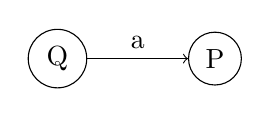
\begin{tikzpicture}
\node (Q) [circle,draw] at (0,1) {Q};
\node (P) [circle,draw] at (2,1) {P};
\draw [->] (Q) -- (P) node[midway,above] {a};
\end{tikzpicture}
\end{center}

\item<2-> \texttt{R} must have a production rule to produce such an \texttt{a}

\item<2-> \texttt{a} must be part of the right hand side of the production rule

\item<3-> We do not know what \texttt{D} may consume after reaching \texttt{P}, but whatever it is it must be generated by production rules obtained from transition rules starting at \texttt{P}

\item<4-> \texttt{a} and anything read after reaching \texttt{P} must be generated

\item<5-> The states of \texttt{D} are the nonterminals of the regular grammar

\item<5-> From \texttt{Q} an \texttt{a} and whatever is produced by \texttt{P} must be produced:
\begin{alltt}
     (list \quot{}Q ARROW \quot{}aP)
\end{alltt}

\end{itemize}
\end{scriptsize}
\end{frame}

\begin{frame}[fragile]
\frametitle{Regular Grammars}
%\framesubtitle{HOMEWORK}
\begin{scriptsize}
\begin{itemize}
\item<1->
\begin{center}
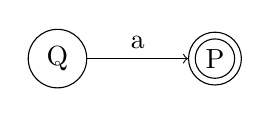
\begin{tikzpicture}
\node (Q) [circle,draw] at (0,1) {Q};
\node (P) [circle,draw] at (2,1) {P};
\draw [->] (Q) -- (P) node[midway,above] {a};
\draw (2,1) circle (0.25cm);
\end{tikzpicture}
\end{center}

\item<2-> Two rules when \texttt{P} is a final state
\begin{alltt}
     (list \quot{}Q ARROW \quot{}a)
     (list \quot{}Q ARROW \quot{}aP)
\end{alltt}

\item<3-> \texttt{D}'s starting state, \texttt{S}, is a final state:
\begin{alltt}
     (list \quot{}S ARROW EMP)
\end{alltt}

\end{itemize}
\end{scriptsize}
\end{frame}

\begin{frame}[fragile]
\frametitle{Regular Grammars}
%\framesubtitle{HOMEWORK}
\begin{scriptsize}
\begin{itemize}
\item<1->
\begin{alltt}
;; (listof dfa-rule) (listof state) \arrow (listof rg-rule)
;; Purpose: Generate production rules for the given
;;          dfa-rules and the given final states
(define (mk-prod-rules mrules mfinals)
\end{alltt}

\item<3->
\begin{alltt}
 (append-map
   (\lamb (r)
     (if (not (member (third r) mfinals))
         (list (list (first r) ARROW (los->symbol (rest r))))
\end{alltt}

\item<4->
\begin{alltt}
         (list (list (first r) ARROW (second r))
               (list (first r) ARROW (los->symbol (rest r))))))
   mrules))
\end{alltt}

\item<2->
\begin{alltt}
;; Tests for mk-prod-rules
(check-equal? (mk-prod-rules \elist \quot{}(F G)) \elist)
(check-equal? (mk-prod-rules \quot{}((S a F) (S b R)
                               (R a G) (R b R)
                               (G a G) (G b G))
                             \quot{}(F G))
              \quot{}((S -> a) (S -> aF) (S -> bR)
                (R -> a) (R -> aG) (R -> bR)
                (G -> a) (G -> aG) (G -> b)  (G -> bG)))
\end{alltt}

\end{itemize}
\end{scriptsize}
\end{frame}

\begin{frame}[fragile]
\frametitle{Regular Grammars}
%\framesubtitle{HOMEWORK}
\begin{tiny}
\begin{itemize}
\item<1->
\begin{alltt}
;; dfa \arrow rg
;; Purpose: Build a rg for the language of the given dfa
;; Assume: dfa states are represented by a single capital letter
(define (dfa2rg m)
\end{alltt}

\item<3->
\begin{alltt}
  (let* [(nts (sm-states m))
         (sigma (sm-sigma m))
         (startnt (sm-start m))
\end{alltt}

\item<4->
\begin{alltt}
         (prules (if (member (sm-start m) (sm-finals m))
                     (cons (list (sm-start m) ARROW EMP)
                           (mk-prod-rules (sm-rules m) (sm-finals m)))
                     (mk-prod-rules (sm-rules m) (sm-finals m))))]
\end{alltt}

\item<5->
\begin{alltt}
    (make-rg nts sigma prules startnt)))
\end{alltt}

\item<2->
\begin{alltt}
;; Tests for dfa2rg
(define SIGMA*-rg (dfa2rg SIGMA*))
(define EA-OB-rg  (dfa2rg EVEN-A-ODD-B))

(check-equal? (eq? (last (grammar-derive SIGMA*-rg \elist)) EMP)
              (eq? (sm-apply SIGMA* \elist) \quot{}accept))
(check-equal? (eq? (last (grammar-derive SIGMA*-rg \quot{}(a b c)))
                   (los->symbol \quot{}(a b c)))
              (eq? (sm-apply SIGMA* \quot{}(a b c)) \quot{}accept))
(check-equal? (eq? (last (grammar-derive SIGMA*-rg \quot{}(c c a b a c)))
                   (los->symbol \quot{}(c c a b a c)))
              (eq? (sm-apply SIGMA* \quot{}(c c a b a c)) \quot{}accept))

(check-equal? (string? (grammar-derive EA-OB-rg \quot{}(a b)))
              (eq? (sm-apply EVEN-A-ODD-B \quot{}(a b)) \quot{}reject))
(check-equal? (string? (grammar-derive EA-OB-rg \quot{}(a a b a)))
              (eq? (sm-apply EVEN-A-ODD-B \quot{}(a a b a)) \quot{}reject))
(check-equal? (eq? (last (grammar-derive EA-OB-rg \quot{}(b)))
                   (los->symbol \quot{}(b)))
              (eq? (sm-apply EVEN-A-ODD-B \quot{}(b)) \quot{}accept))
(check-equal? (eq? (last (grammar-derive EA-OB-rg \quot{}(b a a b b)))
                   (los->symbol \quot{}(b a a b b)))
              (eq? (sm-apply EVEN-A-ODD-B \quot{}(b a a b b))
\end{alltt}

\end{itemize}
\end{tiny}
\end{frame}

\begin{frame}[fragile]
\frametitle{Regular Grammars}
%\framesubtitle{HOMEWORK}
\begin{tiny}
\begin{theorem}
L is regular $\Rightarrow$ L is generated by a regular grammar.
\end{theorem}

\begin{itemize}
\item<1-> M = (make-dfa S \sig{} Z F \delt) decides L

\item<1-> G = (dfa2rg M)

\item<1-> Show that w$\in$L(M) $\Leftrightarrow$ w$\in$L(G) $\wedge$ w$\notin$L(M) $\Leftrightarrow$ w$\notin$L(G)

\item<2-> \underline{w$\in$L(M) $\Leftrightarrow$ w$\in$L(G)}

\item<3-> ($\Rightarrow$) Assume w$\in$L(M)

\item<3-> This means that M performs the following computation: (w Z) \steps$_M$ (() K), where K$\in$F

\item<4-> By construction of G, for every rule, (C a D), in M there is a corresponding production rule (C \arrow{} aD)

\item<4-> In addition, if D is a final state: (C \arrow{} a)

\item<5-> This means that every element consumed by M's computation is generated by a derivation using G simulating M's execution

\item<5-> If M moves to a final state and accepts then the derivation only generates a terminal symbol that is the same symbol consumed by M

\item<6-> Finally, if nothing is consumed and M accepts then the derivation using G generates EMP

\item<6-> This means there is a derivation using G that generates a word accepted by M

\item<6-> Thus, w$\in$L(G)

\item<7-> ($\Leftarrow$) Assume w$\in$L(G)

\item<8-> This means that G can derive w

\item<9-> By construction of G, every derivation step of G simulates a step taken by M in a computation that consumes w and reaches a final state

\item<10> Therefore, w$\in$L(M)

\end{itemize}
\end{tiny}
\end{frame}

\begin{frame}[fragile]
\frametitle{Regular Grammars}
%\framesubtitle{HOMEWORK}
\begin{tiny}
\begin{theorem}
L is regular $\Rightarrow$ L is generated by a regular grammar.
\end{theorem}

\begin{itemize}
\item<1-> M = (make-dfa S \sig{} Z F \delt) decides L

\item<1-> G = (dfa2rg M)

\item<1-> \underline{w$\notin$L(M) $\Leftrightarrow$ w$\notin$L(G)}\\

\item<2-> ($\Rightarrow$) Assume w$\notin$L(M).\\

\item<3-> This means that M's computation on w is (w Z) \steps$_M$ (() K), where K$\notin$F

\item<4-> By construction of G, for every rule, (C a D), in M there is a corresponding production rule (C \arrow{} aD)

\item<5-> That is, a derivation using G simulates the computation done by M

\item<6-> Let (L a K) be the last transition rule M uses during its computation on w

\item<7-> This means that the last production rule G uses is (L \arrow{} aK)

\item<8-> Observe that the symbol produced still represents the existence of a nonterminal and, thus, cannot equal w

\item<9-> Given that G is simulating a \dfa{} and K is not a final state of M, there is no other possible set of derivation steps on w.

\item<9-> Thus, w$\notin$L(G)

\item<10-> ($\Leftarrow$) Assume w$\notin$L(G)

\item<11-> This means that there is no derivation of w using G

\item<12-> By construction, a derivation using G is simulating the computation of M on w

\item<13-> Given that M is deterministic there is only one computation possible

\item<14-> Thus, w$\notin$L(M)

\end{itemize}
\end{tiny}
\end{frame}

\begin{frame}[fragile]
\frametitle{Regular Grammars}
%\framesubtitle{HOMEWORK}
\begin{scriptsize}
\begin{itemize}
\item<1-> Convert \texttt{G=(make-rg N \sig P S)} into, \texttt{M}, a finite-state machine that decides \texttt{L(G)}

\item<1-> The finite-state machine shall simulate a derivation

\end{itemize}
\end{scriptsize}
\end{frame}

\begin{frame}[fragile]
\frametitle{Regular Grammars}
%\framesubtitle{HOMEWORK}
\begin{scriptsize}
\begin{itemize}
\item<1-> \texttt{G}'s nonterminals are states in \texttt{M}

\item<1-> \sig{} is \texttt{M}'s alphabet

\item<1-> \texttt{S} is \texttt{M}'s starting state

\item<2-> If \texttt{M} is to simulate a derivation under \texttt{G} then \texttt{M} must accept when a simple production rule is used

\item<2-> A simple production rule:
\begin{alltt}
     I \(\rightarrow\) i, where i\(\in\)\{\{\ep\}\(\cup\)\sig\} \(\wedge\) I\(\in\)N
\end{alltt}

\item<3-> \texttt{M} shall have, \texttt{Z}, a unique state that is also the single final state:
\begin{alltt}
     I \(\rightarrow\) i  \(\dashrightarrow\) (I i Z)
\end{alltt}

\item<4-> \texttt{M} must also have a transition rule for every compound production rule in \texttt{G}

\item<4-> A compound production rule is defined as follows:
\begin{alltt}
     I \(\rightarrow\) iJ, where i\(\in\)\sig \(\wedge\) I,J\(\in\)N
\end{alltt}

\item<5-> To simulate a compound production rule:
\begin{alltt}
     I \(\rightarrow\) iJ  \(\dashrightarrow\) (I i J)
\end{alltt}

\end{itemize}
\end{scriptsize}
\end{frame}

\begin{frame}[fragile]
\frametitle{Regular Grammars}
%\framesubtitle{HOMEWORK}
\begin{scriptsize}
\begin{itemize}
\item<1-> Consider:
\begin{alltt}
(define a*Ub*-rg   ;; L = a* U b*
 (make-rg \quot{}(S A B) \quot{}(a b)
          \qquot{}((S ,ARROW ,EMP) (S ,ARROW aA) (S ,ARROW bB)
            (S ,ARROW a) (S ,ARROW b) (A ,ARROW aA)
            (A ,ARROW a) (B ,ARROW bB) (B ,ARROW b))
          \quot{}S))
\end{alltt}

\item<2->
\begin{alltt}
     S = (cons \quot{}Z \quot{}(S A B))
     \sig = \quot{}(a b)
     A = \quot{}S
     F = (list \quot{}Z)
\end{alltt}

\item<3->
\begin{alltt}
   I \(\rightarrow\) i rules              I \(\rightarrow\) iJ rules
     (S \(\rightarrow\) \ep)                  (S \(\rightarrow\) aA)
     (S \(\rightarrow\) a)                  (S \(\rightarrow\) bB)
     (S \(\rightarrow\) b)                  (A \(\rightarrow\) aA)
     (A \(\rightarrow\) a)                  (B \(\rightarrow\) bB)
     (B \(\rightarrow\) b)
\end{alltt}

\item<4->
\begin{center}
\includegraphics[scale=0.2]{a-star-U-b-star.png}
\end{center}

\item<4-> It is not difficult to see that it decides \texttt{L = a$^*$ $\cup$ b$^*$}

\end{itemize}
\end{scriptsize}
\end{frame}

\begin{frame}[fragile]
\frametitle{Regular Grammars}
%\framesubtitle{HOMEWORK}
\begin{scriptsize}
\begin{itemize}
\item<1-> To test the constructor:
\begin{alltt}
;; Sample rg
;; L = (a U b U c)*
(define SIGMA*-rg (dfa2rg SIGMA*))

;; L = {w | w has an even number of a and an odd number of b}
(define EA-OB-rg (dfa2rg EVEN-A-ODD-B))

;; L = a* U b*
(define a*Ub*-rg
  (make-rg
    \quot{}(S A B)
    \quot{}(a b)
    \qquot{}((S ,ARROW ,EMP) (S ,ARROW aA) (S ,ARROW bB) (S ,ARROW a)
      (S ,ARROW b)    (A ,ARROW aA) (A ,ARROW a)  (B ,ARROW bB)
      (B ,ARROW b))
    \quot{}S))

;; L = {a aba}
(define a-aba-rg
  (make-rg
    \quot{}(S A B)
    \quot{}(a b)
    \qquot{}((S ,ARROW a)  (S ,ARROW aA)  (A ,ARROW bB) (B ,ARROW a))
    \quot{}S))
\end{alltt}

\end{itemize}
\end{scriptsize}
\end{frame}

\begin{frame}[fragile]
\frametitle{Regular Grammars}
%\framesubtitle{HOMEWORK}
\begin{scriptsize}
\begin{itemize}
\item<1->
\begin{alltt}
;; rg \arrow ndfa
;; Purpose: Build a ndfa for the language of the given \rg{}
(define (rg2ndfa rg)
\end{alltt}

\end{itemize}
\end{scriptsize}
\end{frame}

\begin{frame}[fragile]
\frametitle{Regular Grammars}
%\framesubtitle{HOMEWORK}
\begin{tiny}
\begin{itemize}
\item<1->
\begin{alltt}
;; Tests for rg2ndfa
(define SIGMA*2 (rg2ndfa SIGMA*-rg))  (define EA-OB (rg2ndfa EA-OB-rg))
(define a*Ub*   (rg2ndfa a*Ub*-rg))   (define a-aba (rg2ndfa a-aba-rg))

(check-equal? (eq? (sm-apply SIGMA*2 \elist) \quot{}accept)
              (eq? (last (grammar-derive SIGMA*-rg \elist)) EMP))
     \vdotss{}
(check-equal? (sm-testequiv? SIGMA* SIGMA*2) #t)
(check-equal? (eq? (sm-apply EA-OB \quot{}(a b)) \quot{}reject)
              (string=? (grammar-derive EA-OB-rg \quot{}(a b))
                        "(a b) is not in L(G)."))
(check-equal? (eq? (sm-apply EA-OB \quot{}(b)) \quot{}accept)
              (eq? (last (grammar-derive EA-OB-rg \quot{}(b))) (los->symbol \quot{}(b))))
(check-equal? (sm-testequiv? EVEN-A-ODD-B EA-OB) #t)
     \vdotss{}
(check-equal? (eq? (sm-apply a*Ub* \quot{}(a b)) \quot{}reject)
              (string=? (grammar-derive a*Ub*-rg \quot{}(a b))
                        "(a b) is not in L(G)."))
(check-equal? (eq? (sm-apply a*Ub* \elist) \quot{}accept)
              (eq? (last (grammar-derive a*Ub*-rg \elist)) EMP))
     \vdotss{}
\end{alltt}

\end{itemize}
\end{tiny}
\end{frame}

\begin{frame}[fragile]
\frametitle{Regular Grammars}
%\framesubtitle{HOMEWORK}
\begin{tiny}
\begin{itemize}
\item<1->
\begin{alltt}
;; rg \arrow ndfa
;; Purpose: Build a ndfa for the language of the given \rg{}
(define (rg2ndfa rg)
  (let* [(final-state (generate-symbol \quot{}Z (grammar-nts rg)))
\end{alltt}

\item<2->
\begin{alltt}
         (states (cons final-state (grammar-nts rg)))
         (sigma (grammar-sigma rg))
         (start (grammar-start rg))
         (finals (list final-state))
\end{alltt}

\item<3->
\begin{alltt}
         (simple-prs (filter
                       (\lamb (pr) (= (length (symbol->fsmlos (third pr))) 1))
                       (grammar-rules rg)))
         (cmpnd-prs
          (filter (\lamb (pr) (= (length (symbol->fsmlos (third pr))) 2))
                  (grammar-rules rg)))
\end{alltt}

\item<4->
\begin{alltt}
         (rules (append
                  (map (\lamb (spr)
                         (list (first spr) (third spr) final-state))
                       simple-prs)
                  (map (\lamb (pr)
                         (let [(rhs (symbol->fsmlos (third pr)))]
                           (list (first pr) (first rhs) (second rhs))))
                       cmpnd-prs)))]
\end{alltt}

\item<5->
\begin{alltt}
    (make-ndfa states sigma start finals rules)))
\end{alltt}

\end{itemize}
\end{tiny}
\end{frame}

\begin{frame}[fragile]
\frametitle{Regular Grammars}
%\framesubtitle{HOMEWORK}
\begin{tiny}
\begin{lemma}
S $\rightarrow^+$ w $\Leftrightarrow$ ((a$_1$\dotss{}a$_n$) A) \step$^+$ (() Q), where Q=Z if w ends with a terminal symbol and Q$\in$N if w ends with a nonterminal
\end{lemma}

\begin{itemize}
\item<1-> ($\Rightarrow$) Assume S $\rightarrow^+$ w. \\

\item<1-> We must show that (a$_1$\dotss{}a$_n$ A) \step$^+$ (() Q), where Q=Z if w ends with a terminal symbol and Q$\in$N if w ends with a nonterminal

\item<2-> Induction on, n, the number of steps in the derivation

\item<3-> \underline{Base Case}: n=1

\item<3-> The derivation uses only a single production rule

\item<3-> There are two cases:

\item<3-> If it is a simple production rule, (S $\rightarrow$ a), then w=a. By construction of M, we have that (S a Z)$\in$\delt. Therefore, (a A) \step$^+$ (() Z)=(() Q)

\item<4-> If it is a compound production rule, (S $\rightarrow$ aK), then w=aK

\item<4-> By construction of M, we have that (S a K)$\in$\delt

\item<4-> Therefore, (a A) \step$^+$ (() K)=(() Q)

\item<5-> \underline{Inductive Step}:
\item<5-> Assume: S $\rightarrow^+$ w $\Rightarrow$ (a$_1$\dotss{}a$_k$ A) \step$^+$ (() Q), where Q=Z if w ends with a terminal symbol and Q$\in$N if w ends with a nonterminal, for n=k.

\item<5-> Show: S $\rightarrow^+$ w $\Rightarrow$ (a$_1$\dotss{}a$_{k+1}$ A) \step$^+$ (() Q), where Q=Z if w ends with a terminal symbol and Q$\in$N if w ends with a nonterminal, for n=k+1

\item<6-> Assume S $\rightarrow^+$ w for n=k +1

\item<7-> Given that k$\geq$1, k+1$>$1. This means that the derivation of w is either:

\item<7-> S $\rightarrow$  \dotss{} $\rightarrow$ a$_1$\dotss{}a$_k$U $\rightarrow$ a$_1$\dotss{}a$_k$a$_{k+1}$, where U$\in$N

\item<7-> S $\rightarrow$ \dotss{} $\rightarrow$ a$_1$\dotss{}a$_k$U $\rightarrow$ a$_1$\dotss{}a$_k$a$_{k+1}$V,where U,V$\in$N

\item<8-> By inductive hypothesis, we have:\\
((a$_1$\dotss{}a$_k$a$_{k+1}$) A) \steps ((a$_{k+1}$) U)

\item<9->  If the last production rule used in the derivation is a simple production rule, (U $\rightarrow$ a$_{k+1}$), then by construction of M, (U a$_{k+1}$ Z)$\in$\delt

\item<9-> Therefore, ((a$_1$\dotss{}a$_k$a$_{k+1}$) A) \steps (() Z)=(() Q).\\

\item<10->  If the last production rule used in the derivation is a compound production rule, (U $\rightarrow$ a$_{k+1}$V), then by construction of M, (U a$_{k+1}$ V)$\in$\delt

\item<10-> Therefore, ((a$_1$\dotss{}a$_k$a$_{k+1}$) A) \steps (() V)=(() Q)

\end{itemize}
\end{tiny}
\end{frame}

\begin{frame}[fragile]
\frametitle{Regular Grammars}
%\framesubtitle{HOMEWORK}
\begin{tiny}
\begin{lemma}
S $\rightarrow^+$ w $\Leftrightarrow$ ((a$_1$\dotss{}a$_n$) A) \step$^+$ (() Q), where Q=Z if w ends with a terminal symbol and Q$\in$N if w ends with a nonterminal
\end{lemma}

\begin{itemize}
\item<1-> ($\Leftarrow$) Assume (a$_1$\dotss{}a$_n$ A) \step$^+$ (() Q), where Q=Z if w ends with a terminal symbol and Q$\in$N if w ends with a nonterminal

\item<1-> We must show that S $\rightarrow^+$ w

\item<1-> Induction on, n, the number of transitions in M's computation

\item<2-> \underline{Base Case}: n=1

\item<2-> This means that w ends with a terminal

\item<2-> M's computation is either:\\

(() A) \step{} (() Z) $\vee$ ((a) A) \step{} (() Z)

\item<3-> For the first computation, by construction of M, G must have (S \arrow{} \ep)

\item<4-> For the second computation, by construction of M, G must have (S \arrow{} a)

\item<5-> Therefore, S $\rightarrow^+$ w.\\

\item<6-> \underline{Inductive Step}:

\item<6-> Assume: ((a$_1$\dotss{}a$_n$) A) \step$^+$ (() Q), where Q=Z if w ends with a terminal symbol and Q$\in$N if w ends with a nonterminal $\Rightarrow$ S $\rightarrow^+$ w, for n=k.\\

\item<7-> Show: ((a$_1$\dotss{}a$_n$) A) \step$^+$ (() Q), where Q=Z if w ends with a terminal symbol and Q$\in$N if w ends with a nonterminal $\Rightarrow$ S $\rightarrow^+$ w, for n=k+1.\\

\item<8-> Assume ((a$_1$\dotss{}a$_{k+1}$) A) \step$^+$ (() Q), where Q=Z if w ends with a terminal symbol and Q$\in$N if w ends with a nonterminal. Given that k$\geq$1, k+1$>$1

\item<9-> This means that M's computation on (a$_1$\dotss{}a$_{k+1}$) is:\\

((a$_1$\dotss{}a$_{k+1}$) A) \steps ((a$_{k+1}$) R) \step (() Q)

\item<10-> By inductive hypothesis, we have:\\

 A $\rightarrow^*$ a$_1$\dotss{}a$_{k}$R

\item<11-> The last transition in M's computation has either Q=Z or Q$\neq$Z

\item<12-> If Q=Z then, by construction of G, (R \arrow{} a$_{k+1}$)$\in$P. Therefore, we have:\\

A $\rightarrow^*$ a$_1$\dotss{}a$_{k+1}$

\item<13-> If Q$\neq$Z then, by construction, of M (R \arrow{} a$_{k+1}$Q).

\item<14-> Therefore, we have: A $\rightarrow^*$ a$_1$\dotss{}a$_{k+1}$Q

\end{itemize}
\end{tiny}
\end{frame}

\begin{frame}[fragile]
\frametitle{Regular Grammars}
%\framesubtitle{HOMEWORK}
\begin{scriptsize}
\begin{theorem}
L is generated by a regular grammar $\Rightarrow$ L is regular.
\end{theorem}

\begin{itemize}
\item<1-> A assume L is generated by a regular grammar

\item<2-> Let G be a regular grammar such that L = L(G), let w$\in$L, and let M=(rg2ndfa G)

\item<3-> Given that G can be transformed to M, S $\rightarrow^+$ w $\Leftrightarrow$ (w A) \step$^+$ (() Z)

\item<4-> Given that w is an arbitrary word, M decides L

\item<4-> Thus, L is regular

\end{itemize}
\end{scriptsize}
\end{frame}

\begin{frame}[fragile]
\frametitle{Regular Grammars}
%\framesubtitle{HOMEWORK}
\begin{scriptsize}
\begin{itemize}
\item<1-> HOMEWORK: 9, 10, 11, 12

\item<1-> QUIZ: 7 (due in a week)

\end{itemize}
\end{scriptsize}
\end{frame}



\section{Pumping Theorem for Regular Languages}

\begin{frame}[fragile]
\frametitle{Pumping Theorem for RLs}
%\framesubtitle{HOMEWORK}
\begin{scriptsize}
\begin{itemize}
\item<1-> Variety of techniques to establish that a language, \texttt{L}, is regular

\item<2-> You might already suspect, however, that not all languages in the universe are regular

\item<2-> This belief is likely rooted in the fact that the amount of memory is bounded

\item<2-> Loss of knowledge

\item<2-> It would be foolish, however, to dismiss these models as irrelevant to modern Computer Science

\item<3-> Computers have a finite amount of memory

\item<3-> The finite-state machines that we use on a daily basis are, indeed, quite powerful

\item<3-> Does it surprise you or do you doubt that modern computers are finite-state machines?

\item<4-> Does a finite amount of memory limit what can be computed?

\end{itemize}
\end{scriptsize}
\end{frame}

\begin{frame}[fragile]
\frametitle{Pumping Theorem for RLs}
%\framesubtitle{HOMEWORK}
\begin{tiny}
\begin{itemize}
\item<1-> Consider the following language:
\begin{alltt}
     L = \{a\(\sp{\texttt{n}}\)b\(\sp{\texttt{n}}\)| n\(\geq\)0\}
\end{alltt}

\item<1-> On the surface it appears to be a rather simple and uninteresting language

\item<2-> The problem with \texttt{L} is that \texttt{n} is a natural number of arbitrary size

\item<2-> How can a finite-sate machine read \texttt{n} \texttt{a}s and then read \texttt{n} \texttt{b}s?

\item<3-> You may argue this is easy by implementing a finite-state machine that has a loop to read \texttt{n} \texttt{a}s and then a loop to read \texttt{n} \texttt{b}s:
\begin{center}
\includegraphics[scale=0.2]{anbn-buggyndfa.png}
\end{center}

\item<4-> If we define this machine as \texttt{a2n-b2n} the following tests pass:
\begin{alltt}
     ;; Tests for a2n-b2n
     (check-equal? (sm-apply a2n-b2n \quot{}(b b a a)) \quot{}reject)
     (check-equal? (sm-apply a2n-b2n \elist) \quot{}accept)
     (check-equal? (sm-apply a2n-b2n \quot{}(a b)) \quot{}accept)
     (check-equal? (sm-apply a2n-b2n \quot{}(a a b b)) \quot{}accept)
     (check-equal? (sm-apply a2n-b2n \quot{}(a a a b b b)) \quot{}accept)
\end{alltt}

\item<4-> Should this give us confidence that the machine decides \texttt{L}?

\item<5-> Unfortunately, the answer is an unequivocal no

\item<5-> The tests are not thorough enough:
\begin{alltt}
     (check-equal? (sm-apply a2n-b2n \quot{}(a a)) \quot{}reject)
     (check-equal? (sm-apply a2n-b2n \quot{}(b)) \quot{}reject)
     (check-equal? (sm-apply a2n-b2n \quot{}(a a a b)) \quot{}reject)
\end{alltt}

\item<5-> These tests fail and this should not happen

\item<6-> The machine needs to remember the number of \texttt{a}s

\item<6-> To remember an arbitrary number of \texttt{a}s the machine needs an arbitrary number of states

\item<7-> This strongly suggests that \texttt{L} is interesting because it is not a regular language

\item<7-> In general, how can we tell if a language is not regular?

\end{itemize}
\end{tiny}
\end{frame}

\begin{frame}[fragile]
\frametitle{Pumping Theorem for RLs}
%\framesubtitle{HOMEWORK}
\begin{scriptsize}
\begin{itemize}
\item<1-> Cycles in the transition diagram of a finite-state machine and Kleene stars in a regular expression suggest that there is a repetitive structure

\item<2-> For long enough words repetition must occur 1 or more times

\item<2-> What does this observation suggest?

\item<3-> For long enough words in \texttt{L} there must be a repeated subword

\item<3-> Call the repeated subword \texttt{y}

\item<3-> \texttt{w = xyz}$\in$\texttt{L}

\item<4-> \texttt{xyyz}$\in$\texttt{L}, \texttt{xyyyz}$\in$\texttt{L}, \texttt{xyyyyz}$\in$\texttt{L} and so on are also in the machine's language. The loop is traversed one or more times

\item<5-> It is also the case that \texttt{xz} is in the machine's language

\item<6-> Generalize: \texttt{xy$^{\texttt{i}}$z}$\in$\texttt{L}, where \texttt{i$\geq$0}

\item<6-> If \texttt{w$\in$L} then we can ``pump'' up or down on \texttt{y} and still have a word that is in \texttt{L}

\end{itemize}
\end{scriptsize}
\end{frame}

\begin{frame}[fragile]
\frametitle{Pumping Theorem for RLs}
%\framesubtitle{HOMEWORK}
\begin{scriptsize}
\begin{theorem}
For a regular language, L, there is a word length n$\geq$1 such that any w$\in$L may be written as w=xyz, where y$\neq$\ep{}, $|$xy$|$$\leq$n, and xy$^i$z$\in$L for i$\geq$0.
\end{theorem}

\begin{itemize}
\item<2-> Let us be sure we understand what the theorem is stating

\item<3-> \texttt{w$\in$L} of length greater than or equal to some positive integer, \texttt{n}, may be divided into three parts, \texttt{x}, \texttt{y} and \texttt{z}

\item<4-> \texttt{y} is nonempty

\item<5-> The length of \texttt{xy} cannot be longer than \texttt{n}

\item<5-> That is, \texttt{xy} must be at the beginning of \texttt{w}

\item<6-> What is this theorem good for?

\item<7-> For a concrete \texttt{w$\in$L} that is long enough we must be able to identify a nonempty \texttt{y} that may safely be repeated an arbitrary number of times and still end with a world in \texttt{L}

\item<7-> If such a \texttt{y} does not exists then the language is not regular

\end{itemize}
\end{scriptsize}
\end{frame}

\begin{frame}[fragile]
\frametitle{Pumping Theorem for RLs}
%\framesubtitle{HOMEWORK}
\begin{scriptsize}
\begin{theorem}
For a regular language, L, there is a word length n$\geq$1 such that any w$\in$L may be written as w=xyz, where y$\neq$\ep{}, $|$xy$|$$\leq$n, and xy$^i$z$\in$L for i$\geq$0.
\end{theorem}

\begin{itemize}
\item<1-> Given that L is regular, M=(make-dfa K \sig{} S F \delt) decides L

\item<2-> n=$|$K$|$

\item<2->  w=(a$_1$ a$_2$ \dotss{} a$_n$\dotss{} a$_m$)$\in$L

\item<3-> The first n steps of M's computation on w are as follows:\\
((a$_1$ a$_2$ \dotss{} a$_n$) S) \step{} ((a$_2$\dotss{} a$_n$) Q$_1$) \step{} ((a$_3$\dotss{} a$_n$) Q$_2$) \step{} \dots{} (() Q$_n$)

\item<3-> Observe that the computation has n+1 configurations

\item<4-> Since M only has n states by the pigeonhole principle there must be a repeated state in the computation: Q$_i$=Q$_j$

\item<4-> This means there is a loop in M:\\
((a$_{i}$\dotss{}a$_j$) Q$_{i-1}$) \step{} ((a$_{i+1}$\dotss{}a$_j$) Q$_{i}$) \steps{} (() Q$_i$) \\

\item<5-> Given that i$<$j and M is a \dfa{}, (a$_{i}$\dotss{}a$_j$) is not empty

\item<5-> (a$_{i}$\dotss{}a$_j$) may be removed from w or repeated an arbitrary number of times and the resulting word is still in L

\item<6-> If we define x=(a$_{1}$\dotss{}a$_{i-1}$), y=(a$_{i}$\dotss{}a$_j$), and z=(a$_{j+1}$\dotss{}a$_n$) then xy$^i$z$\in$L

\item<7-> Finally, observe that $|$(a$_{1}$\dotss{}a$_j$)$|$$\leq$n because the loop can contain at most all of M's states

\item<7-> Therefore, $|$xy$|$$\leq$n

\end{itemize}
\end{scriptsize}
\end{frame}

\begin{frame}[fragile]
\frametitle{Pumping Theorem for RLs}
%\framesubtitle{HOMEWORK}
\begin{scriptsize}
\begin{theorem}
     L = \{a\(\sp{\texttt{n}}\)b\(\sp{\texttt{n}}\)$|$n\(\geq\)0\} is not regular
\end{theorem}

\begin{itemize}
\item<1-> Assume L is regular

\item<2-> Let \texttt{M = (make-dfa K \sig{} S F \delt{})} decide \texttt{L}

\item<2-> Let \texttt{n = $|$K$|$}

\item<3-> The pumping theorem requires picking a \texttt{w$\in$L} such that \texttt{$|$w$|$ $\geq$ n}

\item<3-> Let \texttt{w=a$^n$b$^n$}

\item<4-> \texttt{M}'s computation on \texttt{w} must visit at least one state twice

\item<4-> That is, \texttt{w} is long enough

\item<5-> Argue that for any valid choice for \texttt{y} pumping up or down some number of times results in a word not in \texttt{L}

\item<6-> We can observe that \texttt{y} can only contain \texttt{a}s

\item<6-> If it contained any \texttt{b}s then \texttt{$|$xy$|$}  would be too long

\item<7-> Thus, \texttt{y = a$^{\texttt{j}}$}, where \texttt{j $>$ 0}

\item<7-> We may write \texttt{w} as follows:
\begin{alltt}
     w = xyz = a\(\sp{n-j-r}\)a\(\sp{j}\)a\(\sp{r}\)b\(\sp{n}\), where x=a\(\sp{n-j-r}\) \(\wedge\) z=a\(\sp{r}\)b\(\sp{n}\)
\end{alltt}

\item<8-> If we pump up once on \texttt{y} then we get:
\begin{alltt}
     w\quot{}= a\(\sp{n-j-r}\)a\(\sp{2j}\)a\(\sp{r}\)b\(\sp{n}\) = a\(\sp{n+j}\)b\(\sp{n}\)
\end{alltt}

\item<9-> Clearly, w\quot{}$\notin$L

\item<10-> Therefore, the assumption that L is regular is wrong

\end{itemize}
\end{scriptsize}
\end{frame}

\begin{frame}[fragile]
\frametitle{Pumping Theorem for RLs}
%\framesubtitle{HOMEWORK}
\begin{scriptsize}
\begin{theorem}
L = \{a$^n$b$^m$ $|$ n$>$m\} is not regular.
\end{theorem}

\begin{itemize}
\item<1-> Assume L is regular

\item<2-> Let \texttt{M = (make-dfa K \sig{} S F \delt{})} decide \texttt{L}

\item<2-> Let \texttt{n = $|$K$|$}

\item<3-> Let \texttt{w = a$^{n+1}$b$^n$}

\item<4-> Clearly, \texttt{M}'s computation on \texttt{w} must visit at least one state twice

\item<4-> We must now argue that there is an \texttt{i$\geq$0} such that pumping up or down \texttt{i} times results in a word not in \texttt{L}

\item<5-> The only possibility for \texttt{y} is y = a$^p$, where p$>$0

\item<6-> If we pump down once the resulting word is \texttt{w\quot = a$^{n+1-p}$b$^n$}

\item<7-> Observe that \texttt{n+1-p}$\leq$n

\item<7-> Clearly, \texttt{w\quot} is not in L

\item<7-> Therefore, the assumption that L is regular is wrong

\end{itemize}
\end{scriptsize}
\end{frame}

\begin{frame}[fragile]
\frametitle{Pumping Theorem for RLs}
%\framesubtitle{HOMEWORK}
\begin{scriptsize}
\begin{theorem}
L = \{w $|$ w$\in$(a b)$^*$ $\wedge$ w has an equal number of \texttt{a}s and \texttt{b}s\} is not regular
\end{theorem}

\begin{itemize}
\item<1-> It's ok not to use the Pumping Theorem

\item<1-> Use closure properties

\item<2-> Assume L is regular

\item<3-> Consider the following regular language:
\begin{alltt}
     L\quot{} = (concat-regexp
            (kleenestar-reg-exp (singleton-regexp a))
            (kleenestar-reg-exp (singleton-regexp b)))
\end{alltt}

\item<4-> If \texttt{L} is regular then by closure under intersection \texttt{L} $\cap$ \texttt{L\quot{}} is also regular

\item<5-> However, we have that:
\begin{alltt}
     \texttt{L} \(\cap\) \texttt{L\quot{}} = a\(\sp{n}\)b\(\sp{n}\)
\end{alltt}

\item<5-> a$^n$b$^n$ is not regular

\item<5-> Therefore, the assumption that \texttt{L} is regular must be wrong

\end{itemize}
\end{scriptsize}
\end{frame}

\begin{frame}[fragile]
\frametitle{Pumping Theorem for RLs}
%\framesubtitle{HOMEWORK}
\begin{scriptsize}
\begin{itemize}
\item<1-> HOMEWORK: 2--4, 8--11

\end{itemize}
\end{scriptsize}
\end{frame}


\end{document} 